\documentclass{report} % Add the document class
\usepackage{graphicx} % For including graphics like logos
\usepackage{lipsum}   % For dummy text
\usepackage{setspace} % For line spacing
\usepackage{fancyhdr} % For custom headers and footers
\usepackage{geometry} % For page margins
\usepackage{amsmath} % For mathematical equations
\usepackage{enumitem} % For customized lists
\usepackage{amsfonts} % For the \forall symbol
\usepackage{multicol} % For multiple columns if needed
\usepackage{enumitem} % For customizing lists
\usepackage{hyperref} % For hyperlinks for table of contents
\usepackage{acronym} % For defining acronyms
\usepackage{tocbibind} % For adding list of figures, tables to table of contents
\usepackage{tabularx} % For tables
\usepackage{float} % For tables
\usepackage{longtable}%to split tables over multiple pages
\usepackage{array}
\usepackage{booktabs}
\usepackage{caption}
\usepackage{hyperref}
\usepackage{fancyheadings}
%
\pagestyle{fancy}
\fancyhead[R]{
    
\includegraphics[width=0.1\textwidth]{./ReportImages/thws_logo.png} % Adjust path and filename
}
\fancyhead[C]{} 
\fancyhead[L]{} 
\addtolength{\headwidth}{\marginparsep}
\addtolength{\headwidth}{\marginparwidth}

\geometry{top=1in, bottom=1in, left=1in, right=1in} % Set page margins

% Configure the hyperref package to remove red boxes and customize link colors
\hypersetup{
    colorlinks=true,      % Set to true to enable colored links
    linkcolor=black,       % Color for internal links (sections, pages, etc.)
    citecolor=black,       % Color for citation links
    filecolor=black,       % Color for file links
    urlcolor=black         % Color for URL links
}


\begin{document}

% Title Page
\begin{titlepage}
    \centering
    \vspace*{1cm}
    
    \Large \textbf{Technical University of Applied Sciences Würzburg-Schweinfurt (THWS)}\\
    \vspace{0.5cm}
    \Large Faculty of Computer Science and Business Information Systems\\
    \vspace{1cm}
    
    \huge \textbf{Master Thesis}\\
    \vspace{1.5cm}
    
    \Huge \textbf{Electrical Engine Efficiency Prediction  Bypassing PDE Simulator}\\
    \vspace{2cm}
    
    \large \textbf{Submitted to the Technical University of Applied Sciences Würzburg-Schweinfurt in the Faculty of Computer Science and Business Information Systems to
    complete a course of studies in Master of Artificial Intelligence}
    
    \vspace{1cm}
    
    \huge Lilly Abraham\\
    \huge K64889\\
    \vspace{1cm}
    \large Submitted on: 11.12.2024\\
    
    \vfill
    
    \large
    Initial examiner: Prof. Dr. Magda Gregorova\\
    Secondary examiner: Prof. Gracia Herranz Mercedes\\

\end{titlepage}

\newpage % Start a new page


% Including an image on this page
\begin{figure}[h]
    
\includegraphics[width=0.8\textwidth]{./ReportImages/qrcode.png} % Adjust path and filename
    \label{fig:your-image}
\end{figure}

\newpage % Start a new page

\chapter*{Abstract}
\addcontentsline{toc}{chapter}{Abstract}

The thesis explores an approach to predict Key Performance Indicators(KPI)s of topology invariant Interior Permanent Magnet Synchronous Magnets (IPSM) Electric Motors from its geometric, physical and simulation parameters.\\
The KPIs to be predicted are plots on Efficiency grid(3D) and Torque curve(2D).\\
We aim to first parameterize the Electric Motor design such that it is feasible to convert into a tabular representation. \\
Next, we would create a table with relevant attributes and design a Multi Linear Perceptron(MLP) with the table as input and the plots in its numerical format as vectors of values.\\
Additionally we conduct a study to model the task as its graph representation and use Graph Neural Networks(GNN) to predict the KPIs.\\
Then we will regularize the loss functions in a way that would smoothen out the plot curves of the prediction values.\\
After which we will evaluate the predictions with the test target values by experimenting with various hyperparameter tuning settings and as a baseline with the average of the parameters.\\
Finally we will enable the KPI's plot visualisation in a manner presentable to the client Valeo(Automaker Company).\\

\newpage 

\newpage 

\chapter*{Acknowledgement}
\addcontentsline{toc}{chapter}{Acknowledgement}
I would like to thank my supervisor Prof. Dr. Magda Gregorova for her guidance and support throughout the course of this thesis.
Her dedication and commitment to our work has been inspiring to me especially on how we transformed statistical math into modelling that I might have developed a new love for academia. \\
I would also like to express my sincere gratitude to Valeo for providing us with the dataset.
Special thanks are in order to Daniel and Leo for sharing valuable insights of the data from an electromechanical standpoint and for giving me a detailed understanding of my task. \\
I owe my Mother and my Siblings my accomplishments. They have been very instrumental in making it possible for me to pursue a Master's degree outside my home country and for the endless support thoughout.\\
Finally, I humble myself before God Almighty for all his blessings and for giving me the strength to persevere and bring my dreams to fruition.\\

\newpage

\newpage

\begin{spacing}{1.2}
    \tableofcontents
\end{spacing}

\newpage

\newpage

\chapter*{Abbreviations}
\addcontentsline{toc}{chapter}{Abbreviations}
\begin{acronym}[TDMA]
  
    \acro{GNN}{Graph Neural Network}
    \acro{MLP}{Multi Linear Perceptron}
    \acro{KPI}{Key Performance Indicator}
    \acro{EM}{Electric Motor}
    \acro{FEM}{Finite Element Method}
    \acro{CNN}{Convolution Neural Network}
    \acro{2D}{2 Dimension}
    \acro{3D}{3 Dimension}
    \acro{MSE}{Mean Squared Error}
    \acro{RMSE}{Root Mean Squared Error}
    \acro{NaN}{Not a Number}
    \acro{ReLU}{Rectified Linear Unit}
    \acro{GPU}{Graphics Processing Unit}
    \acro{MP}{Message Passing}

\end{acronym}


\newpage

\newpage

\chapter{Introduction} 
In the design of electric motors, vast amounts of data are generated to determine which design of an \ac{EM} fits best to \ac{KPI}s. \\
\ac{KPI}s of an Electric Motor are essential to judge the performance of the motor before it is manufactured. \\
Traditionally these \ac{KPI}s are inferred from a description of an \ac{EM} design via a \ac{FEM} approximating the solutions of the Maxwell’s equations. \\
This process, though well established in the \ac{EM} design, is very time consuming and does not allow for high-throughput engine design optimization. \\
The actual engine data of Valeo is used here as the dataset comprising of multiple variant designs of the Double-V topology.\\

The 3 motor topologies manufactured by Valeo are as below:
\begin{enumerate}
    \item Single V Magnet - Consists of a single V magnet shown in Figure \ref{fig:V1 Magnet}.
    \item Double V Magnet - Consists double V magnets shown in Figure \ref{fig:V2 Magnet}.
    \item Nabla Magnet - Consists of a single V Magnet and a delta magnet shown in Figure \ref{fig:Nabla Magnet}.
\end{enumerate}

\begin{figure}[H]
    \centering
    \begin{minipage}[b]{0.325\textwidth}
        \centering
        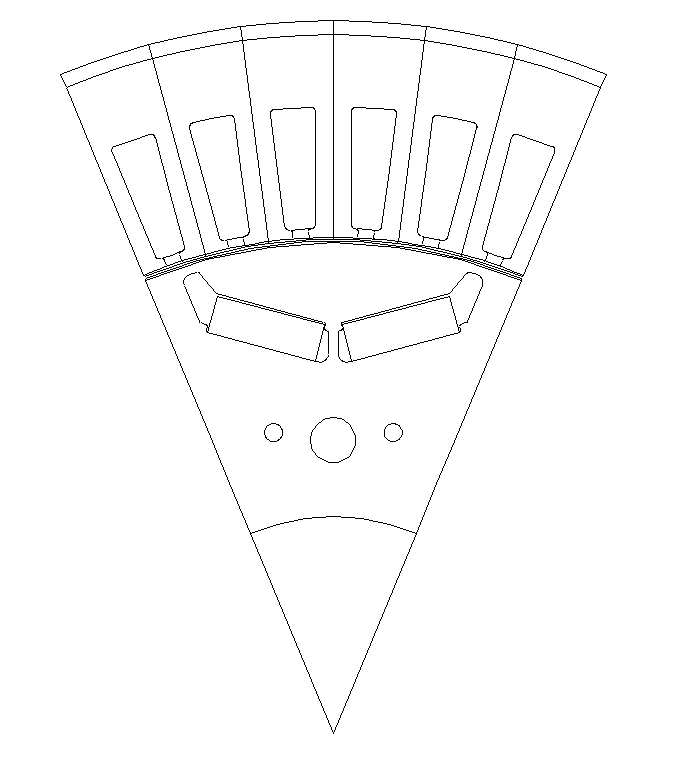
\includegraphics[width=\textwidth]{./ReportImages/1V_Magnet.png}
        \caption{\centering V1 Magnet \\ (Source: Valeo)} % Center the caption here
        \label{fig:V1 Magnet}
    \end{minipage}
    \hfill
    \begin{minipage}[b]{0.325\textwidth}
        \centering
        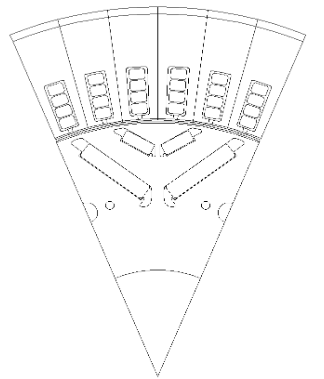
\includegraphics[width=\textwidth]{./ReportImages/2V_Magnet.png}
        \caption{\centering V2 Magnet\\ (Source:Valeo)}
        \label{fig:V2 Magnet}
    \end{minipage}
    \hfill
    \begin{minipage}[b]{0.325\textwidth}
        \centering
        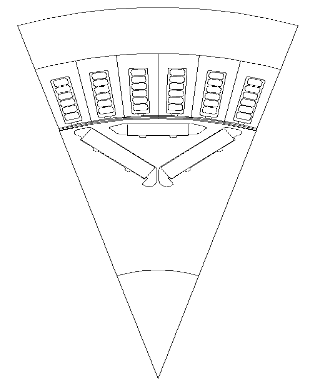
\includegraphics[width=\textwidth]{./ReportImages/Nabla_Magnet.png}
        \caption{\centering Nabla Magnet\\ (Source:Valeo)}
        \label{fig:Nabla Magnet}
    \end{minipage}
\end{figure}

Figure \ref{fig:Torque Curve} and \ref{fig:Efficiency Grid} gives a glimpse of the \ac{EM} \ac{KPI}s to be predicted. \\
\begin{figure}[H]
    \centering
    \begin{minipage}[b]{0.475\textwidth}
        \centering
        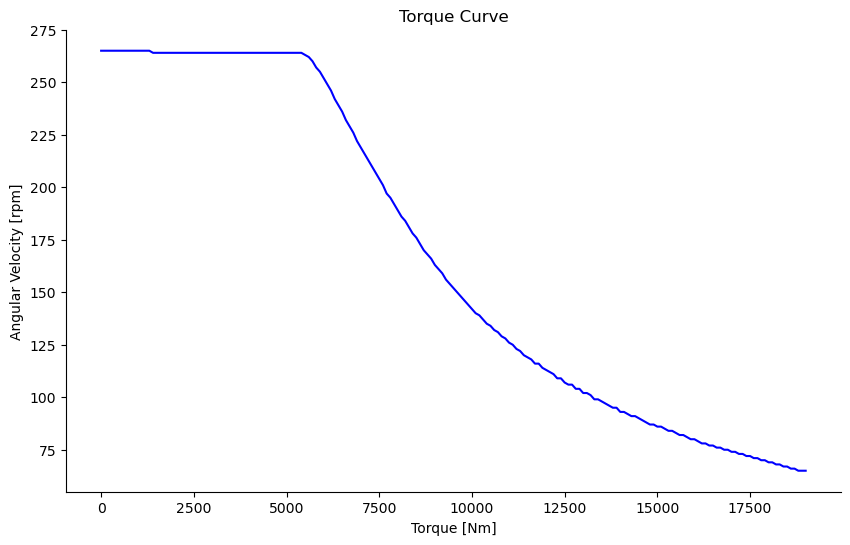
\includegraphics[width=\textwidth]{./ReportImages/TorqueCurve.png}
        \caption{Torque Curve} % Center the caption here
        \label{fig:Torque Curve}
    \end{minipage}
    \hfill
    \begin{minipage}[b]{0.475\textwidth}
        \centering
        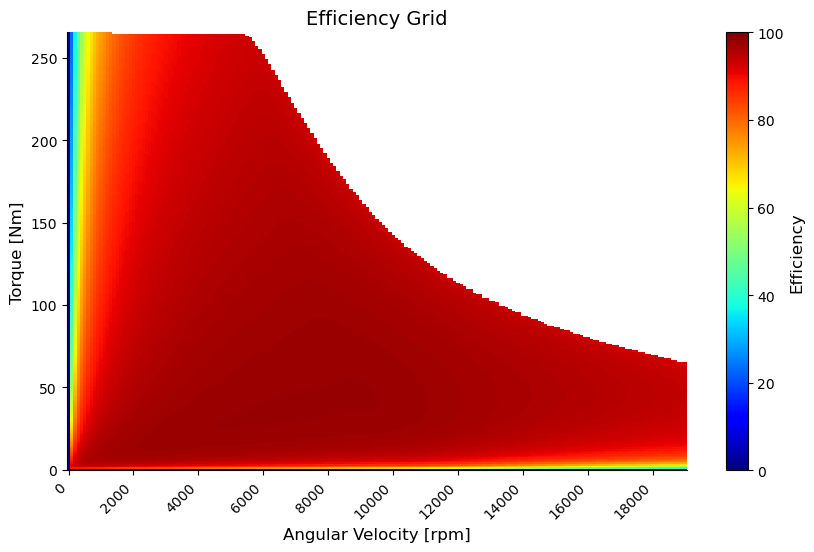
\includegraphics[width=\textwidth]{./ReportImages/EfficiencyGrid.png}
        \caption{Efficiency Grid}
        \label{fig:Efficiency Grid}
    \end{minipage}
\end{figure}

The current approach to predict the \ac{KPI}s of different \ac{EM} design variants is to create a design mesh from the paramteric description of the motor with Matlab.
Multiple FEM simulations which are by nature Partial Differential Equations(PDE) is done on this mesh which is then post processed and the intermediary outputs are forwarded to the Motor Builder.
Several Motor builder settings are then adjusted to get the plots of the desired \ac{KPI}s.\\
This master thesis explores a way to do surrogate modelling of the current process as is highlighted in Figure \ref{fig:EM Design Flowchart} by making use of \ac{GNN} or \ac{MLP} for the modelling of electrical engine designs described parameterically. \\
\begin{figure}[H]
    \centering
    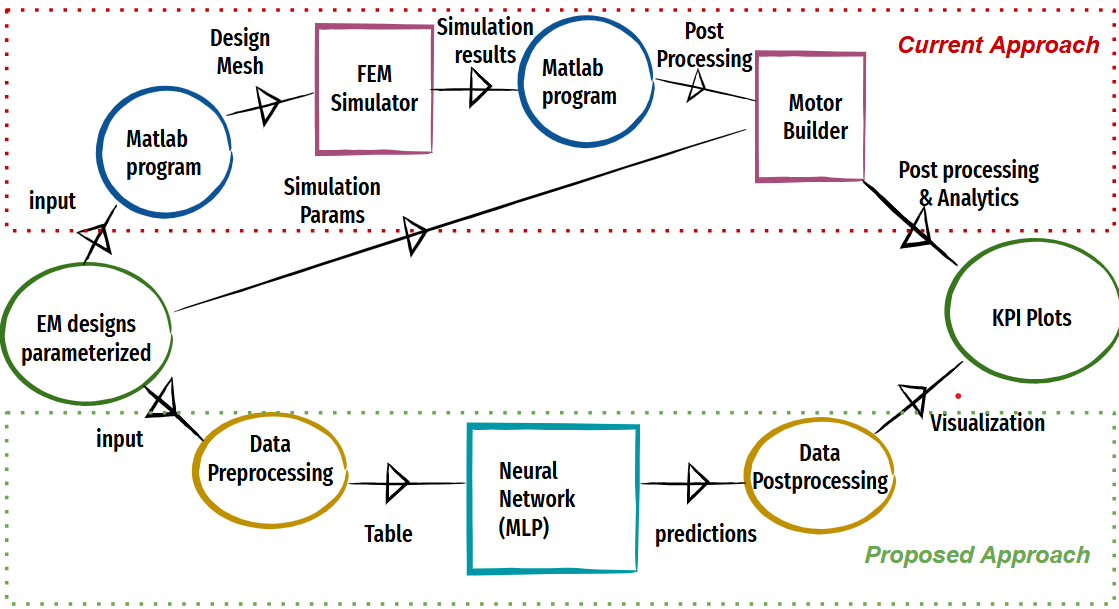
\includegraphics[width=1\textwidth]{./ReportImages/EM_design_flowchart_v2.png} 
    \caption{EM Design Flowchart}
    \label{fig:EM Design Flowchart}
\end{figure}


\section{Objective}\label{sec:Objective}
Our task is to predict 2 KPIs namely the Torque curve and the ETA grid from the parameteric description of topology invariant \ac{EM}. \\ 
The remaining \ac{KPI} such as Losses can be calculated from these 2 KPIs as they are inversely proportional to the Efficiency values.\\
The Torque curve is a 2D plot ie, a vector across speed ranges and the Efficiency grid is a 3D plot ie, a matrix of dimensions torque ranges times speed ranges. \\
Both the outputs are continuous values which makes it a regression problem. \\

\section{Problem Statement}\label{sec:Problem Statement}

\begin{enumerate}

    \item We have a regression problem but as we are predicting two values it makes it a multi regression problem. The model architectures in Section \ref{sec:MLP Model} shines light on how we go about it.
    \item Another concern we came across is the Torque Curve typically harbours integers values however our task is a regression problem and we discuss how we tackle it in Section \ref{sec:MLP Model}. 
    \item The Efficiency grid dimensions vary across \ac{EM} variants, and we need the target from the model to be of a fixed size. This problem is mitigated in Section \ref{sec:Deep Dive into 3D KPI}
    \item The ranges among the 1st and 2nd target vary significantly and is yet another challenge we overcome in Section \ref{sec:Loss for 3D KPI}
    \item Furthermore, we presume graph representation of the data will be more logical than tabular representation due to its ability to grasp the connections within the \ac{EM} structural properties better.
    This would be even more realistic with achieving topology invariance than the tabular representation and conserve memory and compute in the long run.
    However, we realize that our problem cannot be solved using Homogeneous \ac{GNN} which is relatively simpler and is built on a single node and edge type.
    In order to model our problem as a graph, we need to represent it as a Heterogeneous graph. \\

\end{enumerate}

\section{Research Question}\label{sec:Research Question}
\ac{GNN} in general have not been to less explored even so more the heterogeneous \ac{GNN}.
Particularly in the scenario of \ac{EM} Modelling, there has been no publications with \ac{GNN}s.
Hence the need to check its feasibility and its performance with our benchmarks on tabular data.
Additionally, existing Heterogeneous \ac{GNN}s works e.g on recommendation networks, academic networks, information networks, social networks etc involves one large graph with multiple node and edge types. 
However, our problem involves creation of multiple heterogeneous graphs ie, 1 per \ac{EM} variant.\\
Therefore, the applicability of Heterogeneous \ac{GNN}s for our problem is to be seen.\\

We were skeptical on building a model architecture wherein the 2nd KPI is dependent on the 1st KPI as typically the former's shape is dependendent on the latter and not its values.
However we can assume the values within the shape to be non zero values and otherwise 0s and model it in future.\\

Alternatively we could also build 2 models one for each KPIs and thus feed in the dependent predictions when training the latter. \\
However, it would be computationally expensive and does not help in the scenario when we might need to generate \ac{EM} parameteric descriptions.
Additionally we deemed it unnecessary as the dimensions of the ETA grid vary with the torque curve and not necessarily the ETA values. \\

\section{Thesis Structure}\label{sec:Thesis Structure}

Over the course of the thesis we shall refer the Torque curve as Mgrenz KPI and the Efficiency grid as ETA KPI respectively.\\
The thesis is structured to follow sections namely Literature Review, Dataset, Modelling, Experiments and Results, Conclusion, and Bibliography.\\
In Literature Review section will introduce the works that has already been carried out in this domain. \\
In the Dataset section a detailed insight to how our data is structured is elaborated.\\
In the Modelling section, we introduce the methodologies used to tackle the problem. \\
The Experiments and Results chapter gives an outlook on the outcomes of our work in addition to other findings we unearth.\\ 
Conclusion chapter summarizes the thesis briefly and would also give a glimpse into areas of improvement. \\
Finally the Bibliography section lists out the articles cited for this thesis.\\
\newpage 

\chapter{Literature Review} 
There has been extensive research in modeling the Electric Motor with \ac{CNN} based on the images of the motor cross-section. \\
However our approach is progressive in the sense that once the \ac{KPI}s are predicted we would like to be able to generate the inputs.\\
Reproducing images is not known to be the best approach given the infamous known fact that AI generated images are faulty. However by generating the parameters of the motor we can be rest assured of more precise results. \\
Hence the need to focus on the inputs as they are with their parametric description.\\
Existing literature also covers works on modelling this work as tabular data using \ac{MLP}s. 
Although this is fairly good forseeing the impact of generating the inverse process yet \ac{MLP}s cannot necessarily learn all the intricacies within motor components. \\
Hence the need to better represent the data typically in the form of graphs and model \ac{GNN}s to achieve the desired results. \\
There has been close to no work of \ac{GNN}s in this domain. However we see progress of \ac{GNN}s in molecular chemistry and social networks usecases from which we draw inspiration.\\

\newpage 

\chapter{Dataset} 
Valeo an automotive company has supplied the dataset consisting of close to 1500 Double V Electric Motor parameters. 
Around 89 parameters which comprises of the geometric, physical and simulation properties of the motor are chosen among the 196 parameters depending on its overall variability and significance.

Figure \ref{fig:Full Motor} shows the geometry of a whole Double V motor which can be sliced into 8 symmetrical parts.

\begin{figure}[H]
    \centering
    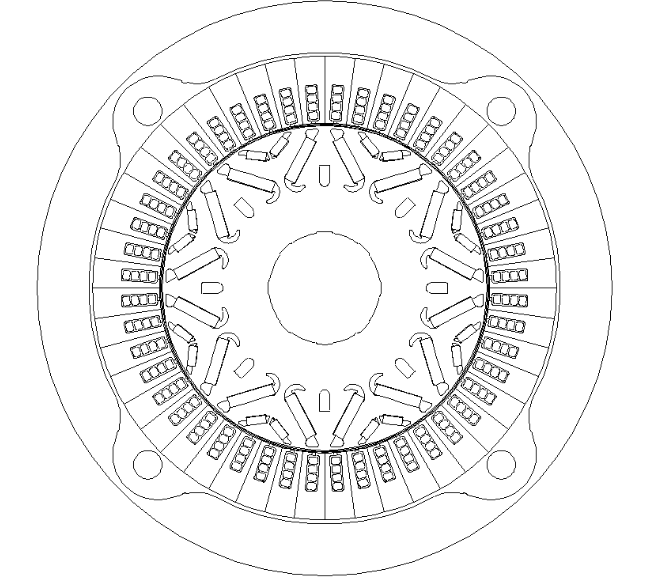
\includegraphics[width=0.5\textwidth]{./ReportImages/FullMotorv2.png} 
    \caption{Complete EM Geometry(Source:Valeo)}
    \label{fig:Full Motor}
\end{figure}

Figure \ref{fig:1/8 Motor Crossection} shows our understanding of how the geometry of 1/8 cross-section of the same motor looks like.
This comes in handy when creating the graph representation of the motor.\\

\begin{figure}[H]
    \centering
    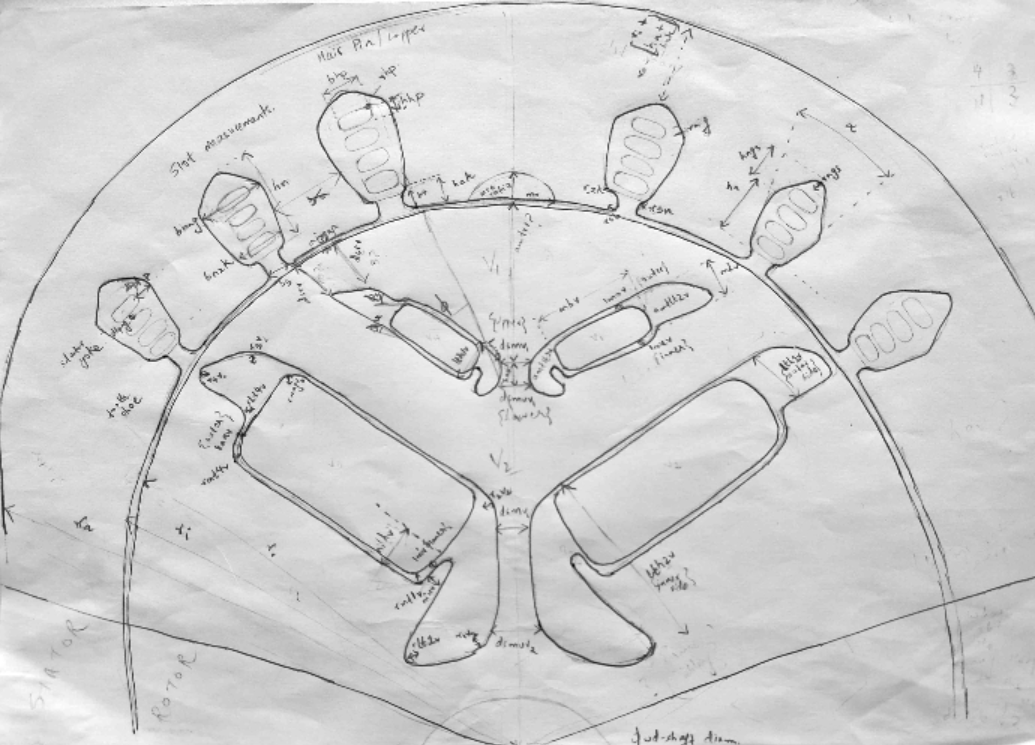
\includegraphics[width=1\textwidth]{./ReportImages/EMCrosssectionFiltered.png} 
    \caption{1/8 Motor Crossection}
    \label{fig:1/8 Motor Crossection}
\end{figure}

\newpage 

Valeo has shared 1481 Excel Workbook files for each motor variant. Each of the excel files contain multiple sheets.
The sheets of interest to us are detailed out in Table \ref{tab:Excel File Structure} :
\begin{table}[H]
    \centering
    \begin{tabular}{|p{2cm}|p{2cm}|p{11cm}|}
    \hline {\bf Sheet} & {\bf Sheet Name} & {\bf Description}\\
    \hline Motor Parameters & input\_data & 
    \begin{itemize}
        \item Contains the input parameters for the motor model.
        \item Includes geometric, physical, and simulation properties.
        \item Unit dimensions if applicable are generally mm or degrees 
    \end{itemize}\\
    Speed Grid & NN & 
    \begin{itemize}
        \item Contains the input parameters for the motor model.
        \item Includes geometric, physical, and simulation properties.
        \item Unit dimensions if applicable are generally mm or degrees 
    \end{itemize}\\
    Torque Grid & MM & 
    \begin{itemize}
        \item Contains the torque grid.
        \item Used for plotting the ETA \ac{KPI}.
    \end{itemize}\\
    ETA Grid & ETA & 
    \begin{itemize}
        \item Contains the ETA \ac{KPI}.
        \item Have the same dimensions as that of NN and MM sheets
    \end{itemize}\\
    Torque Curve & Mgrenz & 
    \begin{itemize}
        \item Contains the values corresponding to Mgrenz \ac{KPI}.
        \item Have the same columns corresponding to the speed grid.
    \end{itemize}\\
    \hline
    \end{tabular}
    \caption{Excel File Structure of an \ac{EM} variant}
    \label{tab:Excel File Structure}
\end{table}



\section{Data Preprocessing for \ac{MLP}}\label{sec:Data Preprocessing for MLP}

For modelling the \ac{MLP}, we present the data in tabular form with the parameters corresponding to columns. \\
In order to make the data compatible with our model, some level of data processing was carried out as elaborated below.

\subsection{Data Exploration of the Input Parameters}\label{sec:Deep Dive into Input Parameters}
All parameters including the additional ones in each topology are considered as a separate columns and therefore if a particular column is topology dependent the data of the other topologies for that corresponding column is treated as 0 values.\\
The values are read and stored in their float equivalent to preserve data precision. \\
Furthermore all degree columns are converted to their equivalent radian values as the latter are directly related to the geometry and makes derivation of other parameters much simpler whereas degrees is a notion of denoting a sliced angle.\\

Table \ref{tab:Input Parameters} shows the input parameters of the motor. 

%Median a column??
\begin{longtable}{|p{1.5cm}|p{1cm}|p{1.5cm}|p{1.5cm}|p{3.5cm}|p{1cm}|p{1cm}|p{1cm}|}

    \hline
    \textbf{Parameter} & \textbf{Unit of Dimension} & \textbf{Mean} & \textbf{Standard Deviation} & \textbf{Value Range} & \textbf{Single V Magnet Topology} & \textbf{Double V Magnet Topology} & \textbf{Nabla Magnet Topology}\\
    \hline
    \endfirsthead
    
    \multicolumn{8}{c}%
    {{\bfseries \tablename\ \thetable{} -- continued from previous page}} \\
    \hline
    \textbf{Parameter} & \textbf{Unit of Dimension} & \textbf{Mean} & \textbf{Standard Deviation} & \textbf{Value Range} & \textbf{Single V Magnet Topology} & \textbf{Double V Magnet Topology} & \textbf{Nabla Magnet Topology}\\
    \hline
    \endhead

    \hline \multicolumn{8}{|r|}{{Continued on next page}} \\ \hline
    \endfoot

    \hline
    \endlastfoot
    \multicolumn{8}{|l|}{\textbf{General Parameters}} \\
    \hline
    N & \# & 4.0 & 0.0 & 4.0--4.0 & \checkmark  & \checkmark & \checkmark  \\
    simQ & \# & 6.0 & 0.0 & 6.0--6.0 & \checkmark  & \checkmark  & \checkmark \\
    r\_a & mm & 9.000000e-02 & 2.554375e-15 & 9.000000e-02--9.000000e-02 & \checkmark  & \checkmark  & \checkmark  \\
    r\_i & mm & 0.064433 & 0.000902 & 0.064000--0.067000 & \checkmark  & \checkmark  & \checkmark  \\
    \hline
    \multicolumn{8}{|l|}{\textbf{Rotor Parameters}} \\
    \hline
    rad\_phiv2 & rad & -0.511319 & 0.063678 & -0.645772--0.000000 & $\times$  & \checkmark & $\times$  \\
    lmsov2 & mm & -0.000289 & 0.000035 &  -0.000300--0.000000 & $\times$  & \checkmark & $\times$  \\
    lth1v2 & mm & 0.005395 & 0.000359 & 0.000000--0.005450 & $\times$  & \checkmark & $\times$  \\
    lth2v2 & mm & 0.002789 & 0.000178 & 0.000000--0.002800 & $\times$  & \checkmark & $\times$ \\
    r1v2 & mm & 0.002097 & 0.000322 & 0.000000--0.002200 & $\times$  & \checkmark & $\times$  \\
    r11v2 & mm & 0.000326 & 0.000040 & 0.000000--0.000600 & $\times$ &\checkmark & $\times$  \\
    r2v2 & mm & 0.001873 & 0.000133 & 0.000000--0.001900 & $\times$  & \checkmark & $\times$  \\
    r3v2 & mm & 0.000697 & 0.000044 & 0.000000--0.000700 & $\times$  & \checkmark & $\times$  \\
    r4v2 & mm &  0.000747 & 0.000048 & 0.000000--0.000750 & $\times$  & \checkmark & $\times$  \\
    rmt1v2 & mm & 0.000249 & 0.000016 & 0.000000--0.000250 & $\times$  & \checkmark &$\times$  \\
    rmt4v2 & mm & 0.000249 & 0.000016 & 0.000000--0.000250 & $\times$  & \checkmark & $\times$  \\
    rlt1v2 & mm & 0.000185 &  0.000045 & 0.000000--0.000200 & $\times$  & \checkmark & $\times$  \\
    rlt4v2 & mm & 0.000249 & 0.000016 & 0.000000--0.000250 & $\times$ & \checkmark & $\times$ \\
    hav2 & mm & 0.004942 & 0.000336 &  0.000000--0.005000 & $\times$  & \checkmark & $\times$  \\
    mbv2 & mm & 0.017706 & 0.001175 & 0.000000--0.018100 & $\times$  & \checkmark & $\times$  \\
    mhv2 & mm & 0.003649 & 0.000265 & 0.000000--0.003800 & $\times$ &\checkmark & $\times$  \\
    rmagv2 & mm & 0.000498 & 0.000032 & 0.000000--0.000500 & $\times$  & \checkmark & $\times$  \\
    dsmv2 & mm & 0.002925 & 0.000194 & 0.000000--0.003100 & $\times$  & \checkmark & $\times$ \\
    dsmuv2 & mm & 0.002925 & 0.000194 & 0.000000--0.003100 & $\times$  & \checkmark & $\times$  \\
    amtrv2 & mm & 0.015888 & 0.001024 & 0.000000--0.016000 & $\times$  & \checkmark & $\times$ \\
    dsrv2 & mm & 0.000996 & 0.000064 & 0.000000--0.001000 & $\times$  & \checkmark & $\times$ \\
    lmav2 & mm & 0.00010 & 0.00003 & 0.00000--0.00011 & $\times$  & \checkmark & $\times$  \\
    lmiv2 & mm & 0.000109 & 0.000008 & 0.000000--0.000110 & $\times$  & \checkmark & $\times$  \\
    lmov2 & mm & 0.000055 & 0.000015 & 0.000000--0.000100 & $\times$  & \checkmark & $\times$  \\
    lmuv2 & mm & 0.000145 & 10.000017 & 0.000000--0.000150 & $\times$  & \checkmark & $\times$ \\
    rad\_phiv1 & rad & -0.694266 & 0.054700 & -0.785398---0.453786 &\checkmark & \checkmark & \checkmark\\
    lmsov1 & mm & -0.000501 & 0.000094 & -0.000530--0.000500 &\checkmark & \checkmark & \checkmark\\
    lth1v1 & mm & 0.002889 & 0.000178 & 0.002855--0.005450 &\checkmark & \checkmark & \checkmark\\
    lth2v1 & mm & 0.002104 & 0.000059 & 0.002100--0.003200 &\checkmark & \checkmark & \checkmark\\
    r1v1 & mm & 0.000407 & 0.000108 & 0.000400--0.002200 &\checkmark & \checkmark & \checkmark\\
    r11v1 & mm & 0.000219 & 0.000045 & 0.000100--0.000600 &\checkmark & \checkmark & \checkmark\\
    r2v1 & mm & 0.000216 & 0.000100 & 0.000200--0.001900 &\checkmark & \checkmark & \checkmark\\
    r3v1 & mm & 0.000899 & 0.000013 & 0.000700--0.000900 &\checkmark & \checkmark & \checkmark\\
    r4v1 & mm & 0.000501 & 0.000016 & 0.000500--0.000750 &\checkmark & \checkmark & \checkmark\\
    rmt1v1 & mm & 2.500000e-04 & 8.839232e-18 & 2.500000e-04--2.500000e-04 &\checkmark & \checkmark & \checkmark\\
    rmt4v1 & mm & 2.500000e-04 & 8.839232e-18 & 2.500000e-04--2.500000e-04 &\checkmark & \checkmark & \checkmark\\
    rlt1v1 & mm & 0.000117 & 0.000056 & 0.000050--0.000250 &\checkmark & \checkmark & \checkmark\\
    rlt4v1 & mm & 2.500000e-04 & 8.839232e-18 & 2.500000e-04--2.500000e-04 &\checkmark & \checkmark & \checkmark\\
    hav1 & mm & 0.002918 & 0.000136 & 0.002900--0.005000 &\checkmark & \checkmark & \checkmark\\
    mbv1 & mm & 0.007643 & 0.000588 & 0.007500--0.018150 &\checkmark & \checkmark & \checkmark\\
    mhv1 & mm & 0.002808 & 0.000140 & 0.002700--0.005000 &\checkmark & \checkmark & \checkmark\\
    rmagv1 & mm & 5.000000e-04 & 1.767846e-17 & 5.000000e-04--5.000000e-04 &\checkmark & \checkmark & \checkmark\\
    dsmv1 & mm & 0.001079 & 0.000141 & 0.000800--0.002800 &\checkmark & \checkmark & \checkmark\\
    dsmuv1 & mm & 0.001079 & 0.000147 & 0.000800--0.002920 &\checkmark & \checkmark & \checkmark\\
    amtrv1 & mm & 0.005538 & 0.000634 & 0.005500--0.019000 &\checkmark & \checkmark & \checkmark\\
    dsrv1 & mm & 0.000752 & 0.000032 & 0.000750--0.001250 &\checkmark & \checkmark & \checkmark\\
    lmav1 & mm & 0.000092 & 0.000026 & 0.000010--0.000110 &\checkmark & \checkmark & \checkmark\\
    lmiv1 & mm & 1.000405e-04 & 6.354235e-07 & 1.000000e-04--1.100000e-04 &\checkmark & \checkmark & \checkmark\\
    lmov1 & mm & 0.000055 & 0.000015 & 0.000050--0.000100 &\checkmark & \checkmark & \checkmark\\
    lmuv1 & mm & 0.000145 & 0.000015 & 0.000100--0.000150 &\checkmark & \checkmark & \checkmark\\
    rad\_phi3b1 & rad & -0.002522 & 0.056001 & -1.256637--0.000000 & $\times$  & $\times$  & \checkmark  \\
    rad\_phi4b1 & rad & -0.000530 & 0.011775 & -0.261799--0.000000 & $\times$  & $\times$  & \checkmark  \\
    lmsob1 & mm & 0.000002 & 0.000034 & 0.000000--0.000750 & $\times$  & $\times$  & \checkmark  \\
    lthb1 & mm & 0.000006 & 0.000128 & 0.000000--0.002900 & $\times$  & $\times$  & \checkmark  \\
    r2b1 & mm & 0.000002 & 0.000045 & 0.000000--0.001000 & $\times$  & $\times$  & \checkmark  \\
    r3b1 & mm & 0.000002 & 0.000034 & 0.000000--0.001000 & $\times$  & $\times$  & \checkmark  \\
    r4b1 & mm & 5.064146e-07 & 1.124422e-05 & 0.000000e+00--2.500000e-04 & $\times$  & $\times$  & \checkmark  \\
    r5b1 & mm & 5.064146e-07 & 1.124422e-05 & 0.000000e+00--2.500000e-04 & $\times$  & $\times$  & \checkmark  \\
    lgr3b1 & mm & 0.000001 & 0.000022 & 0.000000--0.000500 & $\times$  & $\times$  & \checkmark  \\
    lgr4b1 & mm & 6.076975e-07 & 1.349307e-05 & 0.000000e+00--3.000000e-04 & $\times$  & $\times$  & \checkmark  \\
    mbb1 & mm & 0.000030 & 0.000675 & 0.000000--0.015000 & $\times$ & $\times$  & \checkmark \\
    mhb1 & mm & 0.000006 & 0.000144 & 0.000000--0.003200 & $\times$  & $\times$ & \checkmark \\
    mtbb1 & mm & 0.000030 & 0.000675 & 0.000000--0.015000 & $\times$  &$\times$ & \checkmark  \\
    rmagb1 & mm & 0.000001 & 0.000022 & 0.000000--0.000500 & $\times$  & $\times$ & \checkmark \\
    amtrb1 & mm & 0.000004 & 0.000098 & 0.000000--0.002500 & $\times$  & $\times$  & \checkmark  \\
    dsr3b1 & mm & 0.000003 & 0.000066 & 0.000000--0.001850 & $\times$ & $\times$ & \checkmark  \\
    dsr4b1 & mm & 0.000004 & 0.000083 & 0.000000--0.001850 & $\times$  & $\times$  & \checkmark \\
    lmob1 & mm & 2.025658e-07 & 4.497689e-06 & 0.000000e+00--1.000000e-04 & $\times$  & $\times$ & \checkmark \\
    lmub1 & mm & 3.038488e-07 & 6.746534e-06 & 0.000000e+00--1.500000e-04 & $\times$  & $\times$  & \checkmark \\
    lmsub1 & mm & 0.000004 & 0.000081 & 0.000000--0.001800 &$\times$  & $\times$  & \checkmark \\
    \hline
    \multicolumn{8}{|l|}{\textbf{Stator Parameters}} \\
    \hline
    airgap & mm & 1.000000e-03 & 3.535693e-17 & 1.000000e-03--1.000000e-03 &\checkmark  & \checkmark  & \checkmark  \\
    b\_nng & mm & 0.005049 & 0.000091 & 0.004646--0.005120 & \checkmark  & \checkmark  & \checkmark  \\
    b\_nzk & mm & 0.004557 & 0.000057 & 0.004450--0.004646 & \checkmark  & \checkmark  & \checkmark  \\
    b\_s & mm & 0.001002 & 0.000025 & 0.001000--0.001400 & \checkmark  & \checkmark  & \checkmark  \\
    h\_n & mm & 0.011149 & 0.000806 & 0.009200--0.013939 & \checkmark  & \checkmark  & \checkmark  \\
    h\_s & mm & 1.000000e-03 & 3.535693e-17 & 1.000000e-03--1.000000e-03 & \checkmark  & \checkmark  & \checkmark  \\
    r\_sn & mm & 2.500000e-04 & 8.839232e-18 & 2.500000e-04--2.500000e-04 & \checkmark  & \checkmark  & \checkmark  \\
    r\_zk & mm & 0.000501 & 0.000019 & 0.000500--0.000800 & \checkmark  & \checkmark  & \checkmark  \\
    r\_ng & mm & 0.000501 & 0.000019 & 0.000500--0.000800 & \checkmark  & \checkmark  & \checkmark  \\
    h\_zk & mm & 1.000000e-03 & 3.535693e-17 & 1.000000e-03--1.000000e-03 & \checkmark  & \checkmark  & \checkmark  \\
    bhp & mm & 0.003736 & 0.000081 & 0.003550--0.003800 &\checkmark  & \checkmark  & \checkmark  \\
    hhp & mm & 0.002386 & 0.000199 & 0.001900--0.002840 &\checkmark  & \checkmark  & \checkmark  \\
    rhp & mm & 0.000636 & 0.000045 & 0.000500--0.000800 &\checkmark  & \checkmark  & \checkmark  \\
    dhphp & mm & 0.000264 & 0.000014 & 0.000263--0.000485 &\checkmark  & \checkmark  & \checkmark  \\
    dhpng & mm & 0.000406 & 0.000003 & 0.000406--0.000453 &\checkmark  & \checkmark  & \checkmark  \\
    \hline
    \caption{\ac{EM} Input Parameters}
    \label{tab:Input Parameters} \\
\end{longtable}

It gives us a clear idea of how the parameters of the Rotor can vary across Topologies.
In addition the N and simQ parameters are count of Stator poles and its windings respectively and may vary across \ac{EM} variants.\\
1481 examples are of the Double V Magnet Topology apart from which 3 examples each for the other 2 topologies.
Hence, the imbalanced topologies parameters would have relatively not so reliable statistics.\\ 

\subsection{Data Exploration of the Mgrenz \ac{KPI}(Torque Curve)}\label{sec:Deep Dive into 2D KPI}

Figure \ref{fig:Standard Deviation of 2D KPI(ETA) Targets} shows the standard deviation of few samples of the Mgrenz \ac{KPI}.\\

We make the below  observations from it :
\begin{enumerate}
    \item The \ac{RMSE} is at its peak at low speeds.
    \item The curve to an extent resembles a mirrored S shape.
    This finding is critical for how we modelled the loss regularization for the target and will be further elaborated in Section \ref{sec:Loss for 2D KPI}.
\end{enumerate}

\begin{figure}[H]
    \centering
    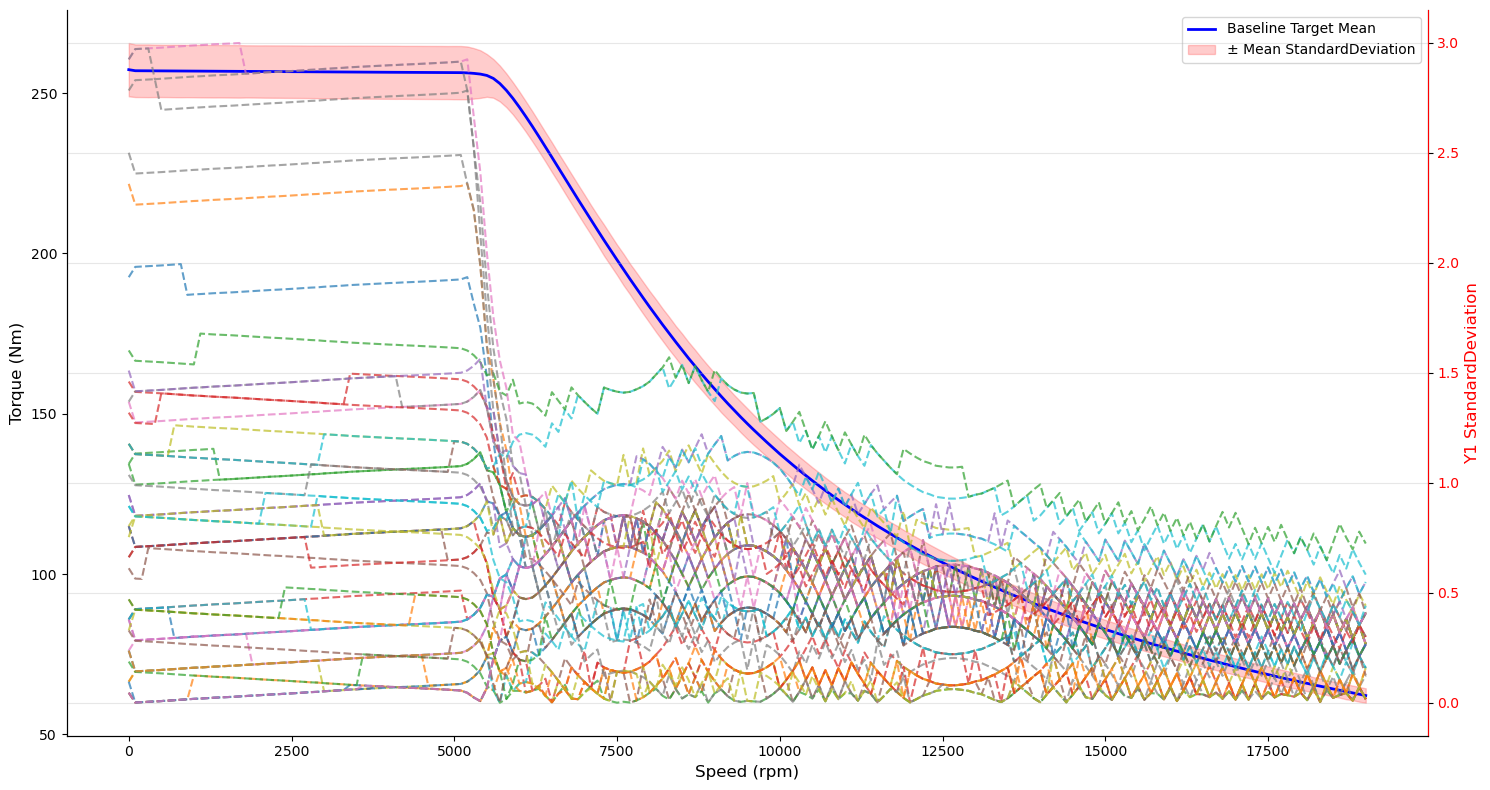
\includegraphics[width=1\textwidth]{./ReportImages/StandardDeviation_Baseline_y1.png} 
    \caption{Standard Deviation of 2D KPI(ETA) Targets} 
    \label{fig:Standard Deviation of 2D KPI(ETA) Targets}
\end{figure}


\subsection{Data Exploration of the ETA \ac{KPI}(Efficiency Grid)}\label{sec:Deep Dive into 3D KPI}

As the target values Mgrenz \ac{KPI} and ETA \ac{KPI} are not provided with the correct dimensions we have an additional step which takes the maximum torque value from the Mgrenz \ac{KPI} and create a similar grid ranging from -maximum torque to maximum torque. \\
We then choose only the rows corresponding to this range from the actual MM grid supplied and the same row indices is used to retrieve the ETA \ac{KPI}. \\
This step ensures that we grant the model the correct dimensions of the ETA \ac{KPI} based on Torque \ac{KPI} and predict likewise.\\

Efficiency values for negative torque values correspond to when motor is in generating mode and those of positive torque values when motor is in monitoring mode.\\
In both modes, the efficiency is almost similar however from Figure \ref{fig:Standard Deviation of 3D KPI(ETA)}, we note it is not the case for our data. 
This is evident from low speed-high torque distribution area where we can see \ac{NaN} values.\\
Since these are FEM simulations, it is probably an effect of a post processing step taken by the Motor builder.
This observation made us decide on dropping the negative ETA \ac{KPI} and only predict the positive ETA \ac{KPI}.\\
The latter can be mirrored in order to obtain the negative ETA \ac{KPI} values if necessary.
It can be mirrored to replicate the efficiency when it is in generating mode.\\

From Figure \ref{fig:Standard Deviation of 3D KPI(ETA) Positive Grid}, we can observe the deviation is at its peak at low torques, low speeds and the border of the curve within the grid.
We discuss the modelling of this information in Section \ref{sec:Loss for 3D KPI}.

Additionally the ETA \ac{KPI} envelope is completely dependent on its equivalent Mgrenz \ac{KPI} curve. 
The area beneath the boundary of which is looked into by the \ac{EM} manufacturers to determine the car's efficiency in the operating cycle.
This is yet another finding we use in Post Processing as is further elaborated in Section \ref{sec:Post Processing}

\begin{figure}[H]
    \centering
    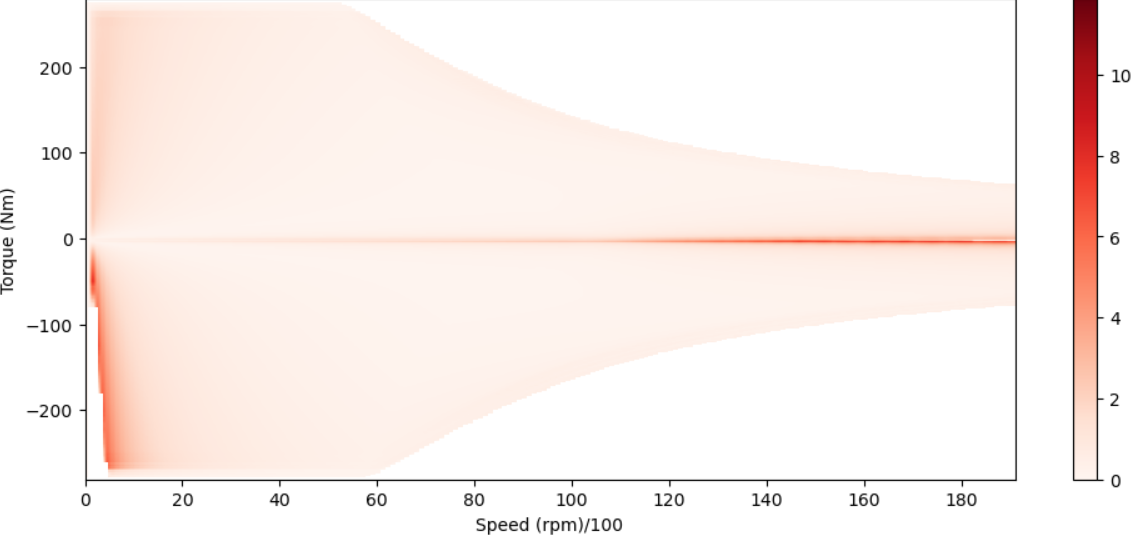
\includegraphics[width=1\textwidth]{./ReportImages/stddev_y2.png} 
    \caption{Standard Deviation of ETA \ac{KPI}} 
    \label{fig:Standard Deviation of 3D KPI(ETA)}
\end{figure}

\begin{figure}[H]
    \centering
    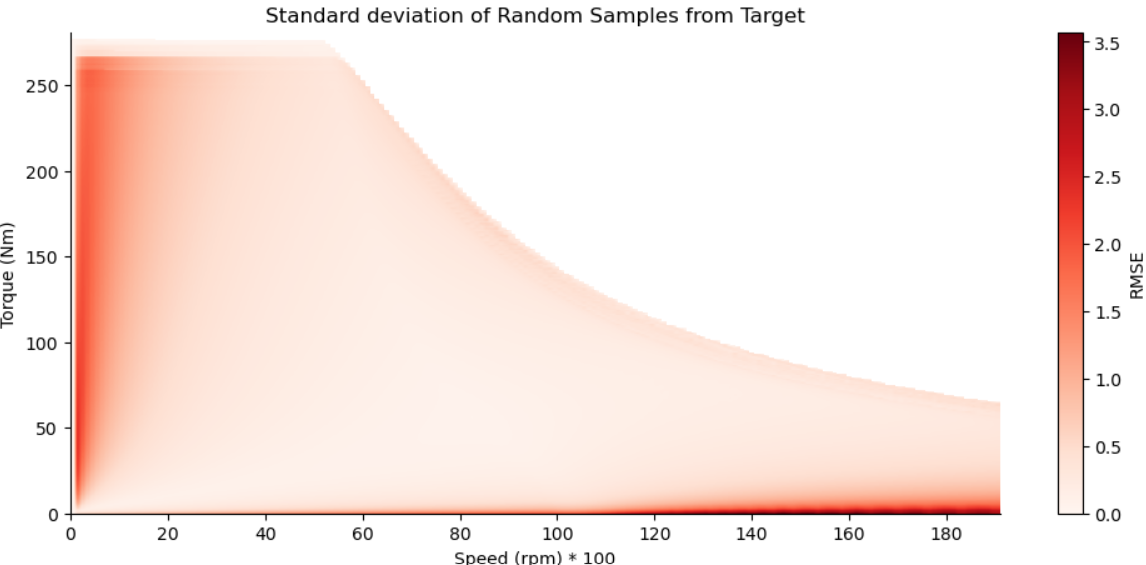
\includegraphics[width=1\textwidth]{./ReportImages/pos_stddev_y2.png} 
    \caption{Standard Deviation of ETA \ac{KPI} Positive Grid} 
    \label{fig:Standard Deviation of 3D KPI(ETA) Positive Grid}
\end{figure}

Figure \ref{fig:Standard Deviation of 3D KPI(ETA) Positive Grid across Speed Intervals} gives us the big picture of how the efficiency values are distributed across equally spaced intervals of speed.
At extreme speeds we find a greater deviation in the efficiency values particularly towards higher speeds. This is because we have fewer efficiency values as speed increases beyond a range and is evident from our targets\\

\begin{figure}[H]
    \centering
    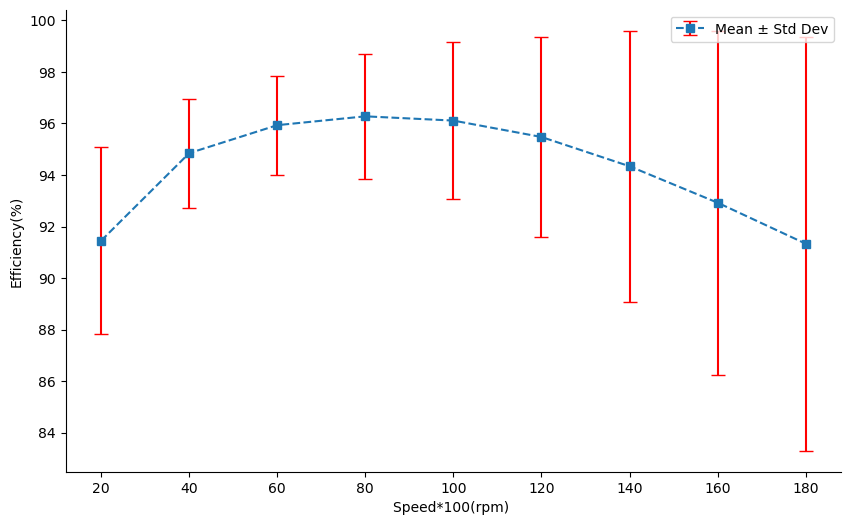
\includegraphics[width=0.8\textwidth]{./ReportImages/stddev_y2_nn_Target.png} 
    \caption{Standard Deviation of ETA \ac{KPI} Positive Grid across Speed Intervals} 
    \label{fig:Standard Deviation of 3D KPI(ETA) Positive Grid across Speed Intervals}
\end{figure}

Due to the infamous fact that reading sheets in excel files take up a lot of time and compute, we read the files as a onetime job when creating the table and store them into pythonic objects for faster access for training.\\
Both the input and target values for the Mgrenz \ac{KPI} is stored locally as csv files whereas those of the ETA \ac{KPI} is stored as separate csv files per variant considering it is in the form of a \ac{2D} array.\\
The csv files are then concatenated and stored into an array conserving dimensionality by padding \ac{NaN} values to match dimensionality of the grid corresponding to the Mgrenz \ac{KPI} with the largest torque value.
In our case the value is 280 but this is subject to change as we receive more data and can be overridden by the user.
The array is then saved locally for easy access and loading during training.\\

Initially  we tried to set it \ac{NaN} values as an incredibly high value hoping the model would consider this as a default value instead of \ac{NaN}.
However, it resulted in poor predictions as the model must have been confused and tried to increase its spread of predictions to cover this large value and so all true values were also predicted to be close to this dummy value.
Fortunately, we have come up with a better way of handling this scenario and we discuss in Section \ref{sec:Loss for 3D KPI} how we tackle it.


\section{Scaling}\label{sec:Scaling}

Scaling is a common practice done before training a neural network. 
Standard scaling is the most prevalent scaling mechanism used for normalization as it results in a Gaussian Distribution centered around the mean. \\
We have used the same for the input features to bring them to a common scale. 

The Scaling is formulated mathematically as in Equation \ref{eq:Standard Scaling}

\begin{equation}
    \text{z} = \frac{x - \mu}{\sigma}
    \label{eq:Standard Scaling}
\end{equation} 

\makebox[\textwidth][c]{%
    \begin{minipage}{0.4\textwidth}
        \centering
        \textit{where
                \begin{itemize}
                    \item x : Input
                    \item $\mu$ : Mean
                    \item $\sigma$ : Standard Deviation
                \end{itemize}
                }
    \end{minipage}
}

\vspace{0.2cm} % Adjusts vertical space between equation and text  

For the Input features both Mean and Standard deviation are calculated across columns. This is attributed to the fact we have columns with different ranges for the input.\\ 

We decided against scaling the targets owing to below 2 reasons :
\begin{enumerate}
    \item They do not enter the network architecture but are only used during loss calculation.
    \item If we scale the target we will have to scale each example from the train dataset and then average the calculated scaling parameters.
    % This in turn would mean 1 scaling parameter i.e, mean and standard deviation each for the entire dataset.
    It is not a good practice to do so as we will have lost a lot of originality in each example and is now introducing noise to new examples.\\
\end{enumerate}

During our experimentations where we initially scaled the targets, we observed that then the network required substantially less effort to learn and consequently lower learning rate and fewer epochs.
Since this comes at a tradeoff of losing precision, we continued with the original targets.\\

\section{Dataset splitting}\label{sec:Dataset splitting}

We convert the data to float tensors for better precision and collate them into a Tensor Dataset.
We have also split the dataset to have about 50 samples for test and the remaining is used for 5 fold cross validation with 80:20 split for training and validation. \\
The reason we have a separate test dataset from the validation is to ensure that there is no data leakage as we do not want to overfit the test dataset with the hyperparameters we choose during training. \\

Within 5 folds, we expect to cover most grounds on training and have good monitoring on the model's performance for each fold.
We have also used Data loaders to split the dataset into batches that fits into our \ac{GPU} memory.


\chapter{Graph Modelling} 

We intended to model our problem as a Graph and solve using a \ac{GNN}. 
We presume this will be a more clever way of representing our usecase in comparision to tabular data..
The idea was to make use of the Graph dynamics in our usecase and aggregate features that are semantically similar.

\ac{GNN}s aim to learn a representation vector for each node using the \ac{MP} algorithm.
\ac{MP} is based on the graph structure and initial node features.
For each node in the graph over each successive hop of its neighbourhood until it has covered the entire graph, the model updates the learned node representation recursively aggregating its neighbour node features.\\
At the end of the \ac{MP} algorithm, each node in the graph would have a good understanding of the other nodes within the same graph.
Therefore the final representation will be rich enough to have captured all the information within the graph and be used for downstream tasks namely :

\begin{enumerate}
    \item Node Classification
    \item Edge Prediction
    \item Graph Prediction
\end{enumerate}


\section{\ac{GNN} Introduction}\label{sec:GNN Introduction}
\ac{GNN}'s can be broadly classified into 2 types :
\begin{enumerate}
    \item Homogeneous \ac{GNN} \\
        Homogeneous \ac{GNN} are designed for graphs with a single type of nodes and edges. \ac{MP} is done for neighbouring nodes and edges over hops until it learns a representation equivalent from its neighbours.\\
        Homogeneous \ac{GNN} are typically build to capture the structural information within a graph.\\
    \item Heterogeneous \ac{GNN}    
        Heterogeneous \ac{GNN} are designed for graphs with different type of nodes and edges. With different types of nodes and edges, also imply difference in features and dimensionality.
        As a single function cannot cater to each type, hence different \ac{MP} and node updating functions needs to be implemented for each edge and node type respectively.\\
        Therefore \ac{MP} is conditioned on the node and edge type thus allowing the flow of information to be more controlled. \\
        In addition to the structural information, Heterogeneous \ac{GNN}s also excel to capture semantic information within the graph.\\
\end{enumerate}

\ac{GNN}s applications range from Recommendation Networks, Academic Networks, Information Networks to Social Networks.\\
These networks are generally represented by a giant graph in which case graph batching, splitting are unique.

However our task requires us to build 1 graph each for each \ac{EM} variant.

\ac{GNN}'s cannot be too deep due to the oversmoothing problem. This is because the \ac{MP} algorith would have already traversed over all hops.
Studies tells us that it can be mitigated by including pre activation residual connections in the network.\\

\section{Heterogeneous \ac{GNN}}\label{sec:Heterogeneous GNN}

A heterogeneous graph can be defined as \( G = \{ V, E, \phi, \psi \} \) \cite{SE HGNN-2023}, where: \\
\( V \) is the set of nodes, with a node type mapping function \( \phi : V \rightarrow T_v \), \\
\( E \) is the set of edges, with an edge type mapping function \( \psi : E \rightarrow T_e \).\\

Each node \( v_i \in V \) is assigned a node type \( c_i = \phi(v_i) \in T_v \). \cite{SE HGNN-2023}\\
Each edge \( e_{t \leftarrow s} \in E \) (denoted \( e_{ts} \) for short) is assigned a relation \( r_{c_t \leftarrow c_s} = \psi(e_{ts}) \in T_e \) (or \( r_{c_t c_s} \) for short), pointing from the source node \( s \) to the target node \( t \). \cite{SE HGNN-2023}\\

The sets of possible node types can be represented as:
\( T_v = \{ \phi(v) : \forall v \in V \} \). \\
The sets of possible edge types can be represented as:
\( T_e = \{ \psi(e) : \forall e \in E \}.\) \\
When \( |T_v| = |T_e| = 1 \), the graph degenerates into a homogeneous graph \cite{SE HGNN-2023}.

GNNs aim to learn a representation vector \( \mathbf{h}^{(L)}_v \in \mathbb{R}^{d_L} \) for each node \( v \) after \( L \)-layer transformations, 
based on the graph structure and the initial node feature \( \mathbf{h}^{(0)}_v \in \mathbb{R}^{d_0} \) \cite{REF HGNN-2021}.

Heterogeneous \ac{GNN} generally work by having separate non linear functions convolve over each edge type during message computation and over each node type when aggregating the learned information. \\

% e two main categories of HGNNs.
% Metapath-based methods (Schlichtkrull et al. 2018; Zhang
% et al. 2019; Wang et al. 2019; Fu et al. 2020) capture the
% structural information of the same semantic first and then
% fuse different semantic information. These models first ag-
% gregate neighbor features at the scope of each metapath to
% generate semantic vectors, and then fuse these semantic vec-
% tors to generate the final embedding vector. Metapath-free
% methods (Zhu et al. 2019; Hong et al. 2020; Hu et al. 2020b;
% Lv et al. 2021) capture structural and semantic information
% simultaneously. These models aggregate messages from a
% node’s local neighborhood like traditional GNNs, but use ex-
% tra modules (e.g. attentions) to embed semantic information
% such as node types and edge types into propagated messages

% findings from \cite{02}
% (1) semantic attention is essential while neighbor attention is not necessary,
% (2) models with a single-layer structure and long metapaths outperform those with multi-layers and short metapaths


% To easily capture structural information, SeHGNN pre-computes the neighbor aggregation in the pre-processing step us-
% ing a light-weight mean aggregator, which removes the overused neighbor attention and avoids repeated neighbor 
% aggregation in every training epoch. To better utilize semantic information, SeHGNN adopts the single- layer structure with long metapaths to extend the recep-
% tive field, as well as a transformer-based semantic fusion module to fuse features from different metapaths.


% Definition 2 Metapaths. A metapath defines a composite
% relation of several edge types, represented as P ≜ c1 ←
% c2 ← . . . ← cl (P = c1c2 . . . cl for short).
% Given the metapath P, a metapath instance p is a node
% sequence following the schema defined by P, represented
% as p(v1, vl) = {v1, e12, v2, . . . , vl−1, e(l−1)l, vl : vi ∈
% V ci , ei(i+1) ∈ Ecici+1 }. In particular, p(v1, vl) indicates the
% relationship of (l−1)-hop neighborhood where v1 is the tar-
% get node and vl is one of v1’s metapath-based neighbors.
% Given a metapath P with the node types of its two
% ends as c1, cl, a metapath neighbor graph GP =
% {V c1 S V cl , EP } can be constructed out of G, where an
% edge eij ∈ EP , ϕ(i) = c1, ϕ(j) = cl exists in GP if and
% only if there is an metapath instance p(vi, vj ) of P in G


% During runtime, the \ac{MP}-\ac{GNN} algorithm would need to iterate over edge type dictionaries during message computation and over node type dictionaries during node updates.


% Graph Convolution Network (GCN) [21 ] is the pioneer of
% GNN models, where the 𝑙𝑡ℎ layer is defined as
% 𝑯 (𝑙) = 𝜎 ( ˆ𝑨𝑯 (𝑙−1) 𝑾 (𝑙) ), (1)
% where 𝑯 (𝑙) is the representation of all nodes after the 𝑙𝑡ℎ layer.
% 𝑾 (𝑙) is a trainable weight matrix. 𝜎 is the activation function, and
% ˆ𝑨 is the normalized adjacency matrix with self-connections.
% Graph Attention Network (GAT) [32 ] later replaces the av-
% erage aggregation from neighbors, i.e., ˆ𝑨𝑯 (𝑙−1) , as a weighted
% one, where the weight 𝛼𝑖 𝑗 for each edge ⟨𝑖, 𝑗⟩ is from an attention
% mechanism as (layer mark (𝑙) is omitted for simplicity)
% 𝛼𝑖 𝑗 =
% exp
% 
% LeakyReLU
% 
% 𝒂𝑇 [𝑾𝒉𝑖 ∥𝑾𝒉𝑗 ]
% 
% Í𝑘 ∈N𝑖 exp LeakyReLU 𝒂𝑇 [𝑾𝒉𝑖 ∥𝑾𝒉𝑘 ] , (2)
% where 𝒂 and 𝑾 are learnable weights and N𝑖 represents the neigh-
% bors of node 𝑖.

% homogeneous GNNs can also handle heterogeneous graphs by simply ignoring the node and edge types.\cite{04}.
%  This could be one of the future works that can be taken for our tasks as part of ablation studiesto benchmark the performance yet again 

% A meta-path is a path with a pre-
% defined (node or edge) types pattern, i.e., P ≜ 𝑛1
% 𝑟1
% −−→ 𝑛2
% 𝑟2
% −−→ · · · 𝑟𝑙
% −→
% 𝑛𝑙+1, where 𝑟𝑖 ∈ 𝑇𝑒 and 𝑛𝑖 ∈ 𝑇𝑣

% Given a meta-path P, we can re-connect the nodes in 𝐺 to get a
% meta-path neighbor graph 𝐺 P . Edge 𝑢 → 𝑣 exists in 𝐺 P if and
% only if there is at least one path between 𝑢 and 𝑣 following the
% meta-path P in the original graph 𝐺


% Linear Transformation. As the input feature of different types of nodes may vary in dimension, we use a linear layer with bias for
% each node type to map all node features to a shared feature space.\cite{04}

% GNNs are hard to be deep due to the over-smoothing and gradient vanishing problems\cite{04}. To mitigate this problem pre activation  residual connection is proposed.


\section{\ac{EM} Heterogeneous \ac{GNN} Model}\label{sec:EM Heterogeneous GNN Model}

We find the Heterogeneous graph to be most apt for our use case with its different node and edge types as it preserves both the structural and semantics of our data. \\
This property is crucial in modelling our use case as we will then have similar node-edge types per topology. \\

\subsection{\ac{EM} Heterogeneous Graph Construction}\label{subsec:EM Heterogeneous Graph Construction}
Inspired by the promising advantages of HGNN, we took the effort of modelling one for only the Double V Magnet Topology.\\
We construct the heterogeneous graph adaptable for each of the \ac{EM} variants as a NetworkX graph.
\begin{enumerate}
    \item Node Types \\
    \( T_v = \{ v, vm, r, s, sw\} \) \\
    The node type mapping functions of each node type in the graph are as follows :
    \begin{enumerate}
        \item \( T_1\) : Rotor Airgap (\textit{v})  \\
        \( \phi = \{ v11, v12, v21, v22\} \)
        \item \( T_2\) : Rotor Magnet (\textit{vm})  \\
        \( \phi = \{ v1m1, v1m2, v2m1, v2m2\} \)
        \item \( T_3\) : Radius (\textit{r})  \\
        \( \phi = \{ rr, ra, o\} \)
        \item \( T_4\) : Stator Poles (\textit{s})  \\
        \( \phi = \{ s1, s2, s3, s4, s5, s6\} \)
        \item \( T_5\) : Stator Windings (\textit{sw})  \\
        \( \phi = \{ s1w1, s1w2, s1w3, s1w4, \\
                     s2w1, s2w2, s2w3, s2w4, \\
                     s3w1, s3w2, s3w3, s3w4, \\
                     s4w1, s4w2, s4w3, s4w4, \\
                     s5w1, s5w2, s5w3, s5w4, \\
                     s6w1, s6w2, s6w3, s6w4\} \)
    \end{enumerate}
    \item Edge Types \\
    \( T_e = \{ a, d1, d2, d4\} \)\\
    The edge type mapping functions of each edge type in the graph are as follows : \\
    \begin{enumerate}
        \item \( T_1\) : Angular/Radian Edges (\textit{a}) 
        \item \( T_2\) : Distance Edge with 1 feature (\textit{d1}) 
        \item \( T_3\) : Distance Edge with 2 feature (\textit{d2}) 
        \item \( T_4\) : Distance Edge with 4 features (\textit{d4})  
    \end{enumerate}
    \item Node Features 
    \item Edge Features 
\end{enumerate}

Figure \ref{fig:HetGraph} shows the heterogeneous graph we constructed
\begin{figure}[H]
    \centering
    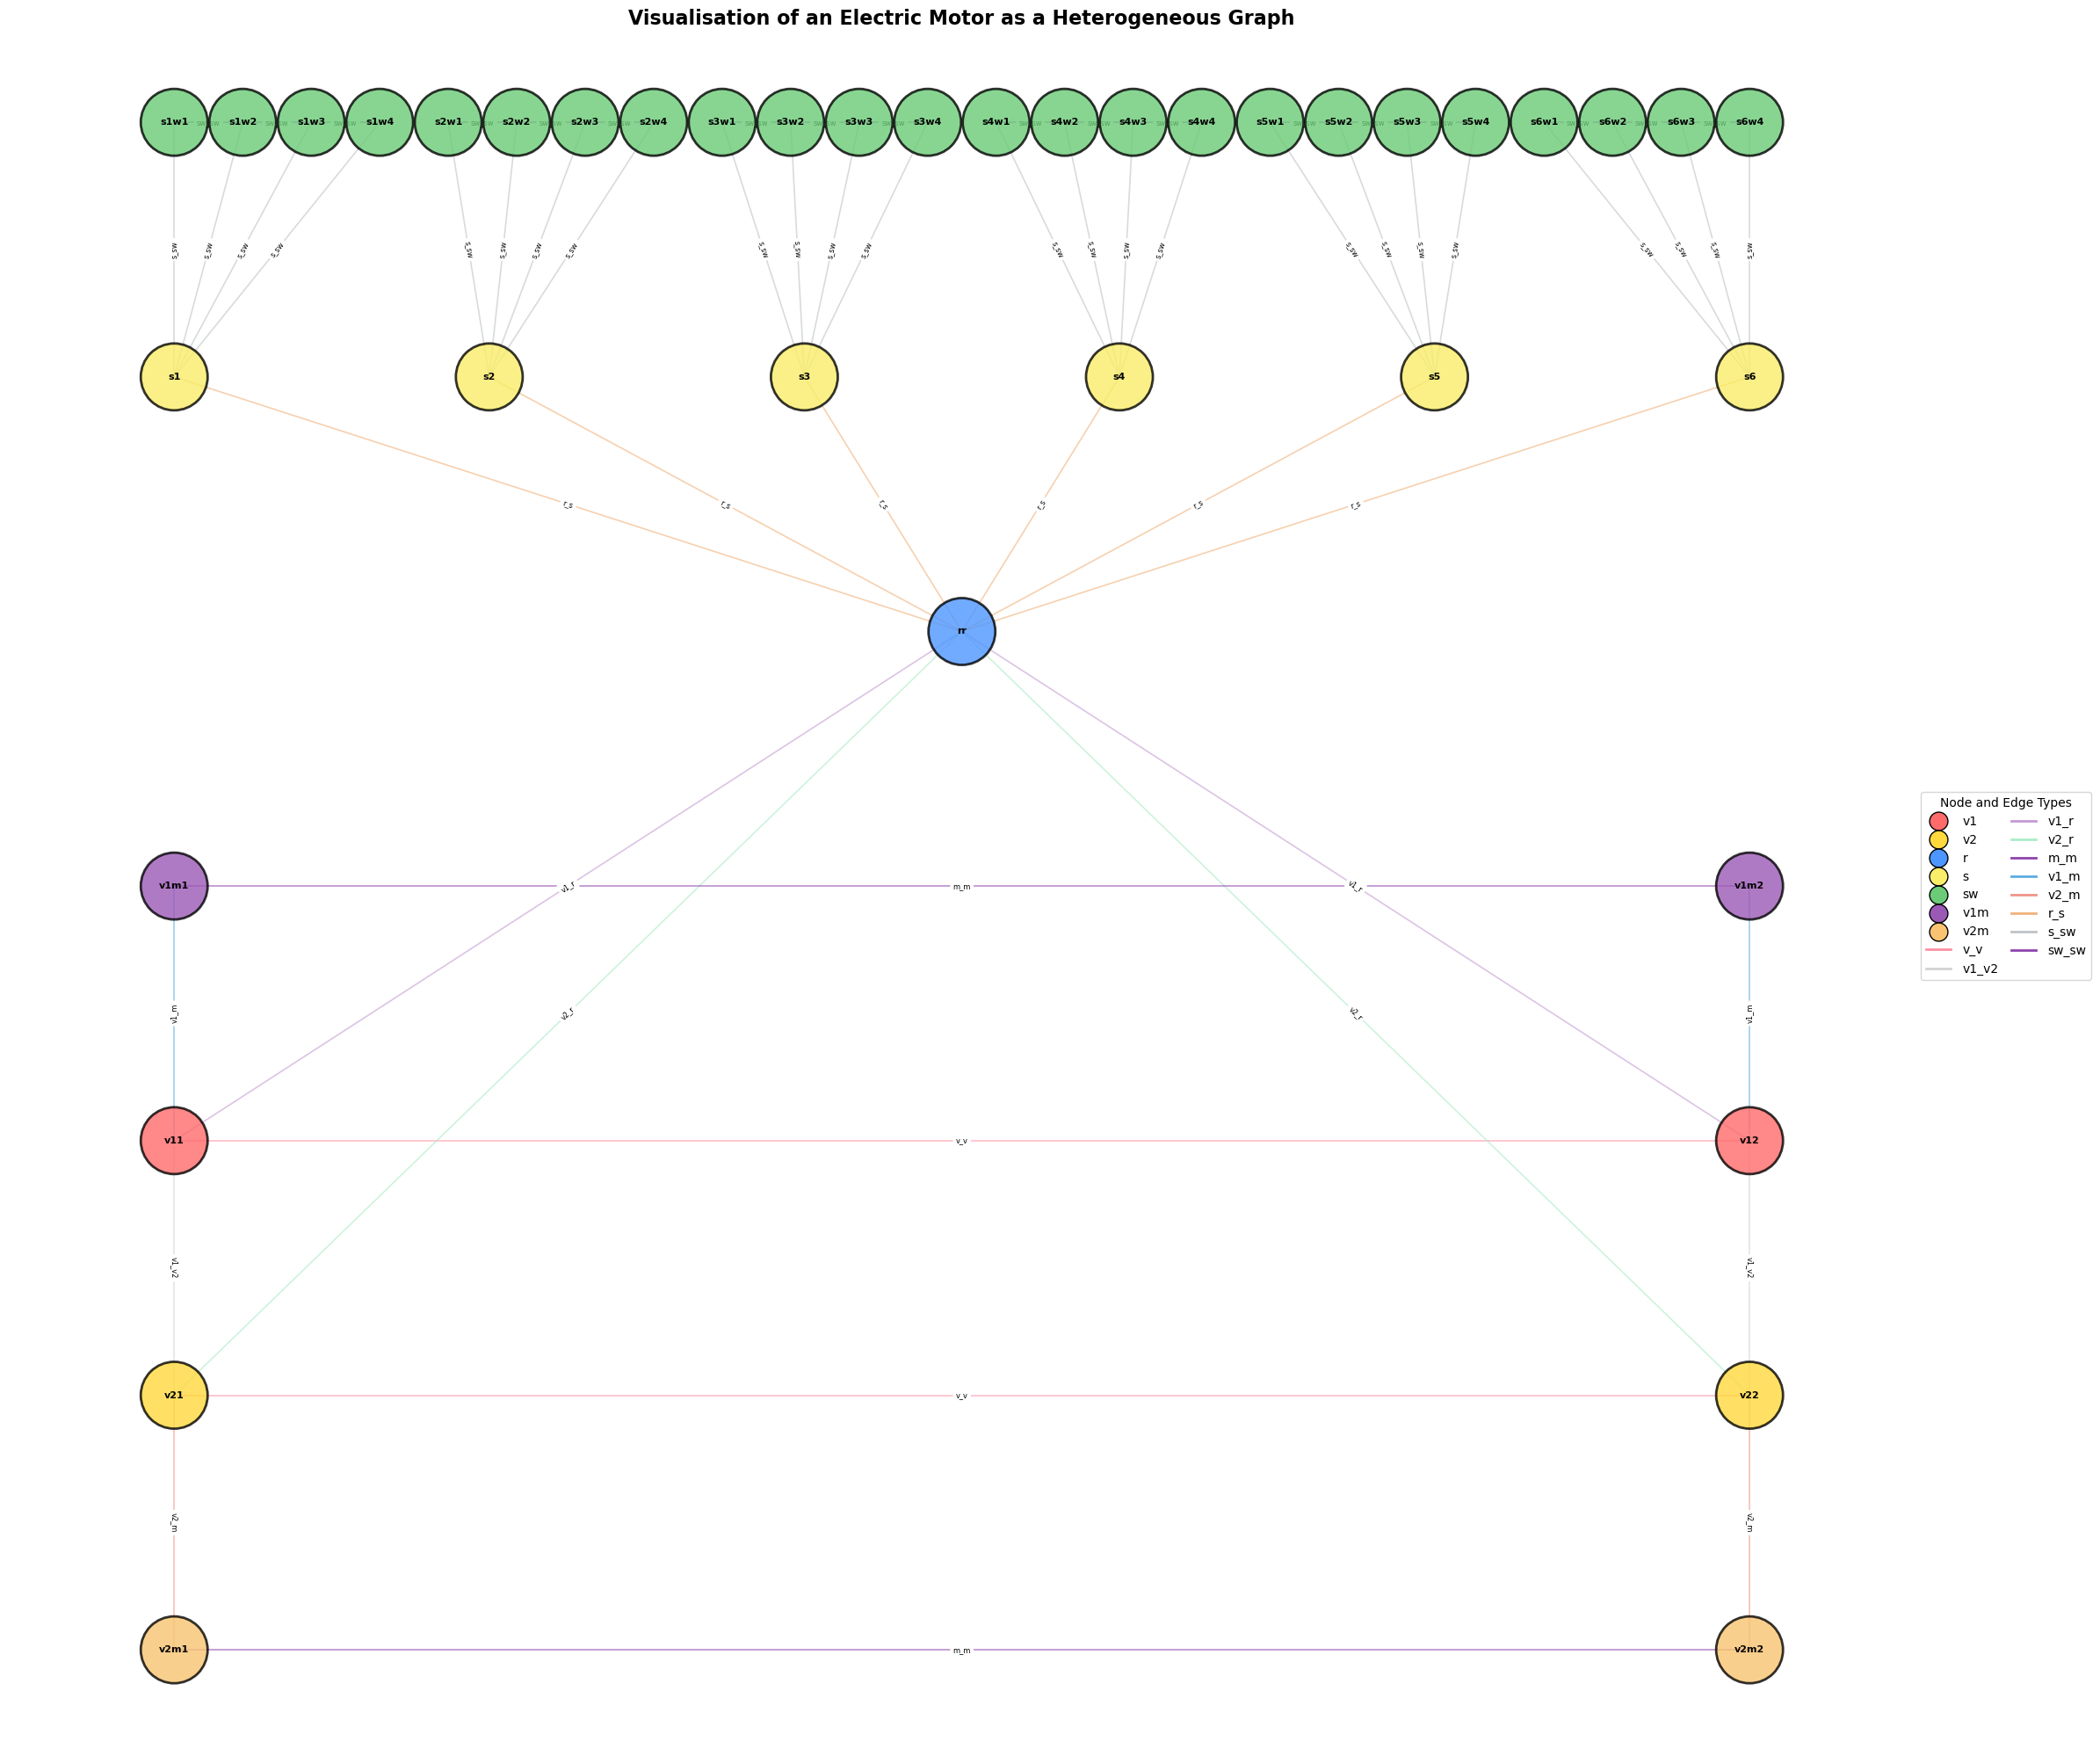
\includegraphics[width=0.9\textwidth]{./ReportImages/graph.png} 
    \caption{HetGraph}
    \label{fig:HetGraph}
\end{figure}
The count of certain parameters within the motor such as stator poles with its corresponding stator windings and rotor magnets is made more comprehendable to the model having new nodes and edges whereas for the \ac{MLP} architecture this information is represented only as a number in yet another column. \\


\newpage 
\chapter{Modelling \& Evaluation}

For our multi regression problem, we first train a \ac{MLP} on the tabular representation of the data and work on it further to do the same with a heterogeneous \ac{GNN}.

\section{\ac{MLP} Model}\label{sec:MLP Model}

For the \ac{MLP} model, we use a single model with input features corresponding to all the features in the tabular topology invariant representation of the data.\\
The model architecture is build to predict both the Mgrenz \ac{KPI} and ETA \ac{KPI}s by having 2 separate output layers for each of the \ac{KPI}s. \\
Since the Mgrenz \ac{KPI}'s targets are relatively learnable than that of the ETA \ac{KPI}'s targets we have experimented with fewer feed forward layers in the former than in the latter. \\
We have a hyperparameter to control the number of neurons in each hidden layer this can be tuned and is further discussed in Section \ref{tab:Hyperparameter Tunings}.\\
% A point of consideration is the hidden size for the shared layers and the MLP Mgrenz layers cannot be varied much. This is further discussed in \ref{tab:Hyperparameter Tunings}.\\
\ac{ReLU} layers were also added in between to serve as the activation function and produce non-linearities and so noise in the network. \\
Dropout layers ensure that not all neurons in each layer are used up during training to prevent the model from memorizing the data and hence overfitting.  
We have 2 hyperparameter to control the dropout rate at which we freeze the neurons when training also to be discussed in Table \ref{tab:Hyperparameter Tunings}.
The 2 dropouts are for shared layers of the \ac{MLP} and for the layers corresponding to ETA \ac{KPI}.\\
Batch normalisation layers are used to normalize the input from the \ac{ReLU} activations applied on it and so mitigate internal covariate shift to the next layer and hence speed up the training process.\\
Thus both batch normalisation and dropout layers stabilize the network training.\\

Figure \ref{fig:MLP Model Architecture} gives an outline on how the \ac{MLP} Model architecture is designed. \\

We discuss each component of the architecture below :
\begin{enumerate}
    \item Input \\
    The input layer takes in all features of the tabular data which is 89 in our case as scaled tensors.
    \item MLP Shared \\
    The MLP Shared block is a sequential block comprising of 2 Linear Layers with the input features and neurons of each hidden layer to be a learnable size we tune.
    We donot increase the number of neurons in the hidden layers within this block as it needs to be in the range of input features and output features(in this case Mgrenz \ac{KPI}).
    Furthermore we have Batch Normalisation layers between each linear and \ac{ReLU} activation function in addition to drop out layers.
    The dropout rate for the layers in this block is relatively higher as we want to encourage the model to focus largely on learning the generality of the data.
    The 2 Linear Layers enable the network at the start to learn a rich represntation of the data at the intial feature extraction phase.
    \item MLP Mgrenz \\
    This block comprises of Sequential 1 Linear Layer with the output feature to be the size of the Mgrenz \ac{KPI} and a \ac{ReLU} activation function.
    We use a \ac{ReLU} activation function at the end of the output layer as the targets are inherently always positive values and it encourages the model to adhere to this fact.
    \item MLP ETA \\
    This block comprises of Sequential 3 Linear Layer with the output feature to be the size of the ETA \ac{KPI}.
    Here we also increase the neurons of the hidden layers as we are not limited by the dimensionality of the output feature.
    This would enable the model to be more strong and grasp the complex patterns in the data better.
    As usual we have batch normalisation, dropout and \ac{ReLU} activation functions between the 1st two Linear layers.
    The dropout rate for the layers in this block is relatively lower as we want to encourage the model to learn the specific nature of the grid towards the end.
    For the Last Linear layer we have the output features corresponding to the target dimensions and a \ac{ReLU} activation again as the targets are inherently always positive values and it again encourages the model to adhere to this fact.
    \item Mgrenz \ac{KPI} \\
    The number of output features correspond to the target size 191.
    Although the targets for the Mgrenz \ac{KPI} are an array of integer values, we use the float tensor and not integer tensor to represent the data else it would become a classification problem and not a regression problem as it should be. \\
    \item ETA \ac{KPI} \\
    The number of output features correspond to the target size which in our case is the shape of the collated array we created as was discussed in Section \ref{sec:Deep Dive into 3D KPI}
\end{enumerate}

\begin{figure}[H]
    \centering
    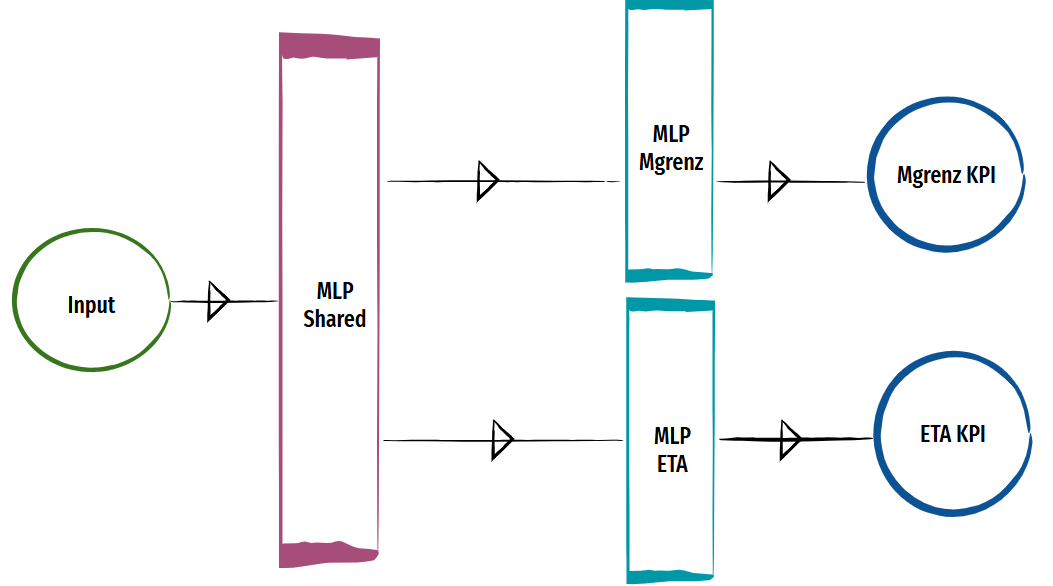
\includegraphics[width=0.8\textwidth]{./ReportImages/mlp_architecture.png} 
    \caption{MLP Model Architecture}
    \label{fig:MLP Model Architecture}
\end{figure}

\section{Loss Functions}\label{sec:Loss Functions}
The \ac{MSE} loss is the loss function used for our problem with the intention that the squared losses penalize the model and inturn encourage it to minimize it further.
In addition to its contribution in exaggerating the loss, \ac{MSE} also ensures that deviations are positive and donot confuse the model by negating the losses of different signs. \\

\subsection{Loss for Mgrenz \ac{KPI}(Torque curve)}\label{sec:Loss for 2D KPI}

The \ac{MSE} loss for the Mgrenz \ac{KPI} is formulated mathematically as in Equation \ref{eq:Y1 Loss}
% Mean Squared Error (\ac{MSE}) Loss for 2D KPI
\begin{equation}
    \text{Y1 Loss} = \frac{1}{n} \sum_{i=1}^{n} \frac{1}{h} \sum_{j=1}^{h} (y_{ij} - \hat{y}_{ij})^2
    \label{eq:Y1 Loss}
\end{equation} 

\makebox[\textwidth][c]{%
    \begin{minipage}{0.4\textwidth}
        \centering
        \textit{where}
        \begin{itemize}
            \item n : \ac{EM} samples
            \item h : Columns of 1D vector
            \item $\hat{y}$ : Prediction
            \item y : Target
        \end{itemize}
    \end{minipage}
}

\vspace{1em} % Adjust the space here, e.g., 1em or 2em


To encourage the model to learn the nature of the curve, we have experimented with 2 Loss Regularization techniques. Both of which are L2 Regularization to be in sync with the dynamics of the \ac{MSE} loss.\\

\begin{enumerate}

    \item Smoothening Loss Regularization \\

To smoothen out the curve for the Mgrenz \ac{KPI} we apply the below loss regularisation factor to take into account.\\
This is formulated mathematically as in Equation \ref{eq:Y1 Smoothening Loss Regularization}.

\begin{equation}
\text{Y1 Smoothening Loss Regularization} = \frac{1}{n} \sum_{i=1}^{n}\frac{1}{h-1} \sum_{j=1}^{h-1} \left(\text{\ac{ReLU}}(|\hat{y}_{i{j+1}} - \hat{y}_{ij}| - 1)\right)^2 
\label{eq:Y1 Smoothening Loss Regularization}
\end{equation} 

\vspace{0.2cm} % Adjusts vertical space between equation and text

This nature is factored in by penalising the loss by the magnitude if the neighbouring values in the prediction are not close to each other.\\
\ac{ReLU} helps to clips the difference if it is negative which is the scenario when a violation is not warranted. \\

\item Decreasing Loss Regularization \\

The Torque curve closely resembles a decreasing sigmoidal curve and hence we use this knowledge to penalize the loss for non-decreasing values within each prediction. \\
This is formulated mathematically as in Equation \ref{eq:Y1 Declining Loss Regularization}.

\begin{equation}
    \text{Y1 Declining Loss Regularization} = \frac{1}{n} \sum_{i=1}^{n}\frac{1}{h-1} \sum_{j=1}^{h-1} \left(\text{\ac{ReLU}}(\hat{y}_{i{j+1}} - \hat{y}_{ij})\right)^2
    \label{eq:Y1 Declining Loss Regularization}
\end{equation} 
    
It takes into consideration the almost continuous decreasing nature of the curve as the regularization is such that a specific element in the array is less than or equal to its prior element. \\

% If the electromagnetic coil is enabled by the commutator for the time span t3, the (almost) maximal current is running through it's loops and the (almost) maximal magnetic field strength is generated. The (almost) maximal torque is acting on the rotor. If the time span is shortened to t2 by increasing rotational speed, a slightly lower torque is acting, because the current through the coil is decreasing slightly. When reducing the time span to t1, the coil gets disconnected from the input voltage even though just half the maximum current is reached. Accordingly the torque decreases significantly:
%[https://homofaciens.de/technics-electric-motors-torque-curve_en.html]
% We add regularization term to help learn the parameters.

\end{enumerate}

We have not combined both the above regularizations as they donot complement each other. This is because the loss regularized by Equation \ref{eq:Y1 Smoothening Loss Regularization} will not necessarily be a decreasing curve.
This holds true for the regularization in Equation \ref{eq:Y1 Declining Loss Regularization} as it may not necessarily have gradual transitions in the curve.
Nevertheless, we perform ablation studies with both the regularizations and report the results obtained in Table \ref{tab:Ablation Studies}

\subsection{Loss for ETA \ac{KPI}(Efficiency Grid)}\label{sec:Loss for 3D KPI}

The \ac{MSE} loss for the \ac{3D} \ac{KPI} is formulated as in Equation \ref{eq:Y2 Loss}.
% Mean Squared Error (\ac{MSE}) Loss for 3D KPI
\begin{equation}
\text{Y2 Loss} = \frac{1}{n} \sum_{i=1}^{n} \frac{1}{w} \frac{1}{h} \sum_{j=1}^{w} \sum_{k=1}^{h} \left( M_{ijk} \cdot y_{ijk}) - (M_{ijk} \cdot \hat{y}_{ijk})\right)^2
\label{eq:Y2 Loss}
\end{equation}

\begin{equation}
    M_{ijk} = \begin{cases}
        1 & \text{if } y_{ijk} \neq \ac{NaN} \\
        0 & \text{if } y_{ijk} = \ac{NaN} 
        \end{cases} \\
\label{eq:Mask matrix}
\end{equation}

\makebox[\textwidth][c]{%
    \begin{minipage}{0.4\textwidth}
        \centering
        \textit{where
                \begin{itemize}
                    \item $M_{ijk}$ : Mask matrix
                    \item w : Rows of \ac{3D} vector
                    \item h : Columns of \ac{3D} vector
                \end{itemize}}
    \end{minipage}
}

\vspace{1em} % Adjust the space here, e.g., 1em or 2em


The ETA \ac{KPI} is a \ac{3D} plot of real numbers representing percentage values and is always in the range of 0-100\%.\\
We noticed in some portions of the ETA \ac{KPI}, the plot not visible as it had \ac{NaN} values.\\
As ANN cannot be trained to predict \ac{NaN} values we have a binary mask constructed such that values corresponding to \ac{NaN} in the target have value 0 and all other values as 1.
Mathematically, this process can be expressed as is in Equation \ref{eq:Mask matrix} and thus ensure that the \ac{NaN} values are ignored in the loss calculation. \\ 
The mask is then multiplied with both the target and its respective prediction. 

Additionally, to encourage the model to learn the nature of the ETA \ac{KPI} from our observations gathered in Section \ref{sec:Deep Dive into 3D KPI}, we have tried to incorporate all of the below learnings via the loss function as Y2 Regularization.\\

\begin{enumerate}

\item Efficiency at Maximum Torque Loss Regularization \\

To ensure that the shape of the ETA \ac{KPI} is maintained, we also regularize the loss for the maximum torque value.
To do so, we have attempted to retrieve the last rows our ETA \ac{KPI} and those of its target values and penalise the squared difference to have higher weight.

We formulate it mathematically as in Equation \ref{eq:Y2_Loss_Regularization_MM_Max_Mgrenz}

\begin{equation}
    \text{Y2 Loss Regularization MM Max Mgrenz} = \frac{1}{n} \sum_{i=1}^{n} \frac{1}{t1} \sum_{j=-t1}^{w} \frac{1}{h} \sum_{k=1}^{h} (y_{ijk} - \hat{y}_{ijk})^2
    \label{eq:Y2_Loss_Regularization_MM_Max_Mgrenz}
\end{equation}

\makebox[\textwidth][c]{%
    \begin{minipage}{0.55\textwidth}
        \centering
        \textit{where
        \begin{itemize}
            \item t1 : Threshold for inital ETA \ac{KPI} Envelope boundary 
        \end{itemize}
        }
    \end{minipage}
}

\vspace{0.2cm} % Adjusts vertical space between equation and text

The number of last rows is determined by a threshold t1

\item Efficiency along the shape of the ETA \ac{KPI} Envelope \\

To ensure that the envelope follows the shape of the Mgrenz \ac{KPI} curve, we penalise the model heavily in case of deviations at the border.
This was developed by considering the last columns for each row of the ETA grid and penalising the squared difference with that of the target.

We formulate it mathematically as in Equation \ref{eq:Y2_Loss_Regularization_Envelope}

\begin{equation}
    \text{Y2 Loss Regularization Envelope} = \frac{1}{n} \sum_{i=1}^{n} \frac{1}{w} \sum_{j=1}^{w} \frac{1}{t2} \sum_{k=-t2}^{h} (y_{ijk} - \hat{y}_{ijk})^2
    \label{eq:Y2_Loss_Regularization_Envelope}
\end{equation}

\makebox[\textwidth][c]{%
    \begin{minipage}{0.4\textwidth}
        \centering
        \textit{where
                \begin{itemize}
                    \item t2 : Threshold for ETA \ac{KPI} Envelope
                \end{itemize}
                }
    \end{minipage}
}

\vspace{0.2cm} % Adjusts vertical space between equation and text


The number of last rows is determined by a threshold t2

\item Efficiency at low speeds \\

To force the model to pay more attention at lower speeds, we have regularized the loss for the first few columns of each row of the ETA grid and penalise the squared difference with that of the target.

We formulate it mathematically as in Equation \ref{eq:Y2_Loss_Regularization_Low_Speed}:

\begin{equation}
    \text{Y2 Loss Regularization Low Speed} = \frac{1}{n} \sum_{i=1}^{n} \frac{1}{w} \sum_{j=1}^{w} \frac{1}{t3} \sum_{k=1}^{t3} (y_{ijk} - \hat{y}_{ijk})^2
    \label{eq:Y2_Loss_Regularization_Low_Speed}
\end{equation}

\makebox[\textwidth][c]{%
    \begin{minipage}{0.4\textwidth}
        \centering
        \textit{where
                \begin{itemize}
                    \item t3 : Threshold for Low Speed
                \end{itemize}
                }
    \end{minipage}
}

\vspace{0.2cm} % Adjusts vertical space between equation and text

The number of first columns is determined by a threshold t3. \\
It is a known fact that at 0 Torque, the corresponding efficiency values for the motor is 0. With this regularization, this learning as well is incorporated into the loss function.\\

\item Efficiency at low Torque \\

To force the model to be more careful at low torque, we have regularized the loss for the first few rows of each column of the ETA \ac{KPI} and penalise the squared difference with that of the target.

We formulate it mathematically as in Equation \ref{eq:Y2_Loss_Regularization_Low_Torque}:

\begin{equation}
    \text{Y2 Loss Regularization Low Torque} = \frac{1}{n} \sum_{i=1}^{n} \frac{1}{t4} \sum_{j=1}^{t4} \frac{1}{h} \sum_{k=1}^{h} (y_{ijk} - \hat{y}_{ijk})^2
    \label{eq:Y2_Loss_Regularization_Low_Torque}
\end{equation}

\makebox[\textwidth][c]{%
    \begin{minipage}{0.4\textwidth}
        \centering
        \textit{where
                \begin{itemize}
                    \item t4 : Threshold for High Torque
                \end{itemize}
                }
    \end{minipage}
}

\vspace{0.2cm} % Adjusts vertical space between equation and text

The number of first rows is determined by a threshold t4

\end{enumerate}

The above Y2 Regularizations are indeed purely \ac{MSE} but with higher weights for specific regions of the ETA \ac{KPI}.
Consequently being L2 Regularizations it goes hand in hand with \ac{MSE} Loss calculated in Equation \ref{eq:Y2 Loss}.\\

We aggregate all the above regularizations to form the Y2 Loss Regularization as in Equation \ref{eq:Y2 Loss Regularization}

\begin{equation}
    \begin{split}
\text{Y2 Loss Regularization} = \text{Y2 Loss Regularization MM Max Mgrenz} + \text{Y2 Loss Regularization Envelope} \\
    + \text{Y2 Loss Regularization Low Speed} + \text{Y2 Loss Regularization Low Torque}
    \end{split}
    \label{eq:Y2 Loss Regularization}
\end{equation}


\vspace{0.2cm} % Adjusts vertical space between equation and text

The Total Loss is calculated in Equation \ref{eq:Total Loss}

\vspace{0.2cm} % Adjusts vertical space between equation and text

\begin{equation}
    \begin{split}
\text{Total Loss} = \text{wt} \times (\text{Y1 Loss} + (\lambda_{\text{1y1}} \times \text{Y1 Smoothening Loss Regularization}) + \\
(\lambda_{\text{2y1}} \times \text{Y1 Declining Loss Regularization })) + \text{(1-wt)} \times (\text{Y2 Loss} + (\lambda_{\text{y2}} \times \text{Y2 Loss Regularization}))
    \end{split}
    \label{eq:Total Loss}
\end{equation}

\makebox[\textwidth][c]{%
    \begin{minipage}{0.6\textwidth}
        \centering
        \textit{where}
        \begin{itemize}
            \item $\lambda_{\text{1y1}}$ : Y1 Smoothening Loss Regularization Parameter
            \item $\lambda_{\text{2y1}}$ : Y1 Declining Loss Regularization Parameter
            \item $\lambda_{\text{y2}}$ : Y2 Loss Regularization Parameter
            \item wt: Y1 Loss Weightage
            \item 1-wt: Y2 Loss Weightage
            % \item $w_{\text{y2}}$: Y2 Loss Weightage
        \end{itemize}
    \end{minipage}
}

\vspace{1em} % Adjust the space here, e.g., 1em or 2em

We have added a Weightage parameter that controls the contribution of the Y1 Loss and Y2 Loss to the Total Loss. There are 2 reasons why this is useful for us :\\

\begin{enumerate}
    \item  When the targets are not of the same scale. \\
    Without scaling, the losses for both targets being of different ranges are drastically different.\\
    We circumvent this by weighing up the loss of the target not performing better on validation dataset and weighing down the loss of the targets by the factor of how much its value range varies. \\
    \item When the prediction accuracy of one \ac{KPI} is substantially more important than the other. \\
    Our task demands the same as the ETA \ac{KPI} is post processed to be within the shape of the Mgrenz \ac{KPI}. \\
    Therefore, in theory have higher weightage for the Mgrenz \ac{KPI} as its loss in performing well is costlier but as its value range is relatively higher we make decisions from monitoring the perdiction performances.\\
    We reflect on these decisions based on whether the envelope of the ETA \ac{KPI} grid is more valuable that the efficiency values within it.\\
    To counter the Mgrenz \ac{KPI} loss dominating the total loss, we have implemented quite a few regularization techniques to the ETA \ac{KPI} loss.\\
    Ultimately we decided on prioritizing the efficiency values itself as we incorporate the envelope shape of the grid as part of the loss regularization in Equation \ref{eq:Y2_Loss_Regularization_Envelope}.\\
    Neverthelss we donot remove the post processing step even so as it guarantees us that values outside the envelope donot appear.
\end{enumerate}
Furthermore, the weightage parameters for both target is designed to sum upto 1 keeping in mind improved training stability as a result of normalized weights. \\

Finally the aggregated loss is backpropagated.\\
\vspace{0.2cm} % Adjusts vertical space between equation and text

\section{Optimizer}\label{sec:Optimizer}

Adam optimizer is used for optimization as it is known to be computationally efficient and requires little memory \cite{ADAM-2017}. \\
It infers the gradients of the loss and how it impacts the weights and biases of each layer and thus guide the model to decrease the loss. \\
The optimizer acts once the loss is backpropagated across training each batch of the dataset.\\
The optimizer also uses the learning rate to control the step size with which the model parameters are updated.\\

\section{Evaluation Metrics}

The evaluation metrics we have considered for our regression problem is the average of the \ac{RMSE}. \\
Therefore, the model with the least prediction scores ie, closest to 0 is ideal for our application. \\

\subsection{Evaluation Metrics for Mgrenz \ac{KPI}}\label{sec:Evaluation Metrics for 2D KPI}

The Y1 Score for the Mgrenz \ac{KPI} is formulated in Equation \ref{eq:Y1 Score} :
% Evaluation metric (\ac{MSE}) Loss for 2D KPI
\begin{equation}
\text{Y1 score} = \frac{1}{n} \sum_{i=1}^{n} \underbrace{ \sqrt{\frac{1}{h} \sum_{j=1}^{h} (y_{ij} - \hat{y}_{ij})^2}}_{Y1\ RMSE}
\label{eq:Y1 Score}
\end{equation}

\makebox[\textwidth][c]{%
    \begin{minipage}{0.45\textwidth}
        \centering
        \textit{where
                \begin{itemize}
                    \item h : Columns of 1D vector
                    \item Y1 \ac{RMSE}: \ac{RMSE} for each test sample
                \end{itemize}
                }
    \end{minipage}
}

\vspace{0.2cm} % Adjusts vertical space between equation and text

\subsection{Evaluation Metrics for ETA \ac{KPI}}\label{sec:Evaluation Metrics for 3D KPI}

The Y2 score for the ETA \ac{KPI} is formulated in Equation \ref{eq:Y2 Score} :
%  Evaluation metric (\ac{MSE}) Loss for 3D KPI
\begin{equation}
    \text{Y2 score} = \frac{1}{n} \sum_{i=1}^{n} \underbrace{ \sqrt{\frac{1}{w} \frac{1}{h} \sum_{j=1}^{w} \sum_{k=1}^{h} (y_{ijk} - \hat{y}_{ijk})^2}}_{Y2\ RMSE}
    \label{eq:Y2 Score}
\end{equation}
    

\makebox[\textwidth][c]{%
    \begin{minipage}{0.45\textwidth}
        \centering
        \textit{where
                \begin{itemize}
                    \item w : Rows of 2D vector
                    \item h : Columns of 2D vector
                    \item Y2 \ac{RMSE} : \ac{RMSE} for each test sample
                \end{itemize}
                }
    \end{minipage}
}

\vspace{0.2cm} % Adjusts vertical space between equation and text

\section{Post Processing}\label{sec:Post Processing}

The mean and standard deviation from the train-validation datasets are applied to transform the test dataset to maintain uniformity in the predictions generated.
In the case of new files we first convert it into the tabular representation our model consumes and then apply the scaling.\\
Hence the reason why we preserve the same scalers used during training as we not only evaluate our dedicated test dataset but also for clients to use on demand. \\

Furthermore as we are predicting a padded matrix to ensure dimensionality sync across different ETA \ac{KPI}'s, the grid contains values even outside the boundary of the ETA \ac{KPI}.
Hence, we attempted to slice the shape of the Mgrenz \ac{KPI} curve from the ETA \ac{KPI} by counting the number of columns a row to have based on consecutive values in the curve.
This brings us back to the point that it is imperative the prediction of the Mgrenz \ac{KPI} is close to perfect as the envelope of the ETA \ac{KPI} inherently is dependent on it.

\newpage 
\newpage 

% Masking NaN values
\chapter{Experiments and Results}

\section{Experiments with \ac{MLP}}\label{sec:Experiments with MLP}

The learnable parameters were chosen via a random grid search  and was tuned by monitoring the model's performance across 5 fold cross validation training.\\
The splits are saved locally and can be used later to ensure reproducibility.

\begin{table}[H]
    \centering
    \begin{tabularx}{1\linewidth}{|X|X|X|}
    \hline {\bf Hyperparameters} & {\bf Description} & {\bf Value}\\
    \hline 
    lr & Learning Rate & 0.075 \\
    hidden size & Dimensionality of Hidden Layers& 128 \\
    lr gamma & Exponential Learning Rate Scheduler Gamma Parameter & 0.9 \\
    batch size & Batch Size & 72 \\
    epochs & Number of Epochs & 10 \\
    py1 & Dropout Probability for Shared Layers & 0.35 \\
    py2 & Dropout Probability for ETA Layers & 0.2 \\
    lambda1 y1 & Y1 Smoothening Curve Loss Regularizer & 0.5 \\
    lambda2 y1 & Y1 Decreasing Curve Loss Regularizer & 0.5 \\
    lambda y2 & Y2 Loss Regularizer & 3.75 \\
    t1 & Y2 Initial Envelope Boundary Threshold & 51 \\
    t2 & Y2 Envelope Threshold & 10 \\
    t3 & Y2 Low Speed Threshold & 20 \\
    t4 & Y2 Low Torque Threshold & 20 \\
    wt & Weightage of Y1 Loss & 0.05 \\
    1-wt & Weightage of Y2 Loss & 0.95 \\
    \hline
    \end{tabularx}
    \caption{Hyperparameter Tuning}
    \label{tab:Hyperparameter Tunings}
\end{table}

We are using an exponential learning rate scheduler which reduces the learning rate exponentially by the \textit{lr gamma parameter} to decay learning as training progresses across epochs.
This is to ensure that the model does not overshoot after few cycles of training.\\
The \textit{batch size} is limited to the capacity of our \ac{GPU} memory. We use the maximum batch size to train faster.\\
The \textit{hidden size} refers to the number of neurons in the hidden layers of the \ac{MLP} model. 
We have experimented with 2 hidden sizes 64 and 128 and donot go beyond.
Reason being we are constrained with the fact that the number of neurons must be between the range of input features and output features which was discussed in Section \ref{sec:MLP Model}.
In addition to it being of the multiples of 8 as \ac{GPU}s are most optimized for the same.
Dropout rate during training is controled by the parameter \textit{py1} for shared layers and \textit{py1} for layers specific to ETA \ac{KPI}. This is discussed in Section \ref{sec:MLP Model}. \\
We donot concern much about the data being dropped in larger extent than anticipated for the Mgrenz \ac{KPI} because it is relatively simpler to learn and the value range is comparitively larger leading its loss to dominate the total loss.\\
\textit{Lambda1 y1}, \textit{lambda2 y1} and \textit{lambda y2} parameters control the regularization weight for the regularization terms for the Mgrenz \ac{KPI} and ETA \ac{KPI} respectively detailed in Equation \ref{eq:Total Loss}.\\
The thresholds \textit{t1}, \textit{t2}, \textit{t3} and \textit{t4} are used to control the number of rows and/or columns to be considered for the regularization terms for the ETA \ac{KPI} as detailed in Section \ref{sec:Loss for 3D KPI}.\\
The weightage parameter to control the direction of loss is denoted by \textit{wt} and is also discussed in Equation \ref{eq:Total Loss}.\\

We chose \texttt{Wandb}\footnote{Weights \& Biases} to log metrics from the training run and to monitor model performance across the 5 folds. \\
Our \ac{MLP} model only uses the loss regularization parameters \textit{lambda2 y1} and \textit{lambda y2} ie, it does not conider the Smoothening curve Regularization fot the Mgrenz \ac{KPI}s.
\begin{figure}[H]
    \centering
    \begin{minipage}[b]{0.325\textwidth}
        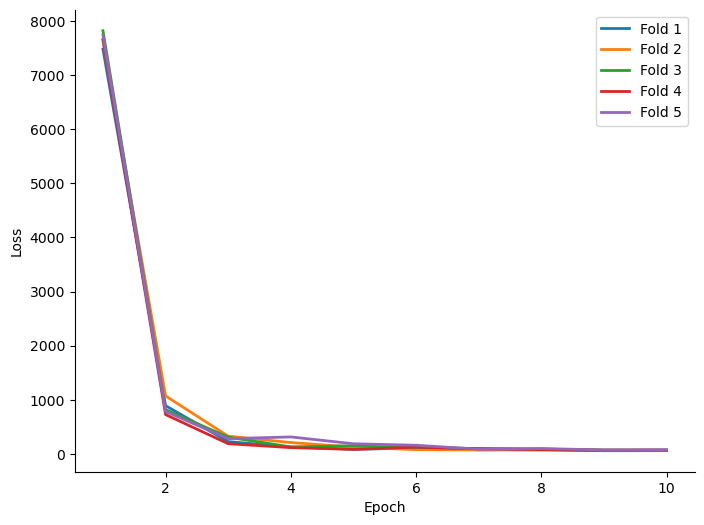
\includegraphics[width=\textwidth]{./ReportImages/train_loss.png}
        \caption{\centering Aggregated Training Loss}
        \label{fig:Aggregated Training Loss}
    \end{minipage}
    \hfill
    \begin{minipage}[b]{0.325\textwidth}
        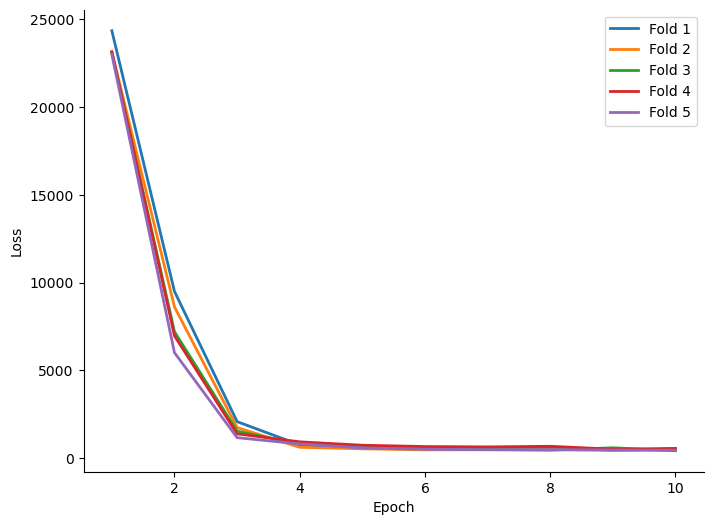
\includegraphics[width=\textwidth]{./ReportImages/train_loss_y1.png}
        \caption{\centering Training Loss for Mgrenz \ac{KPI}}
        \label{fig:Training Loss for Torque Curve}
    \end{minipage}
    \hfill
    \begin{minipage}[b]{0.325\textwidth}
        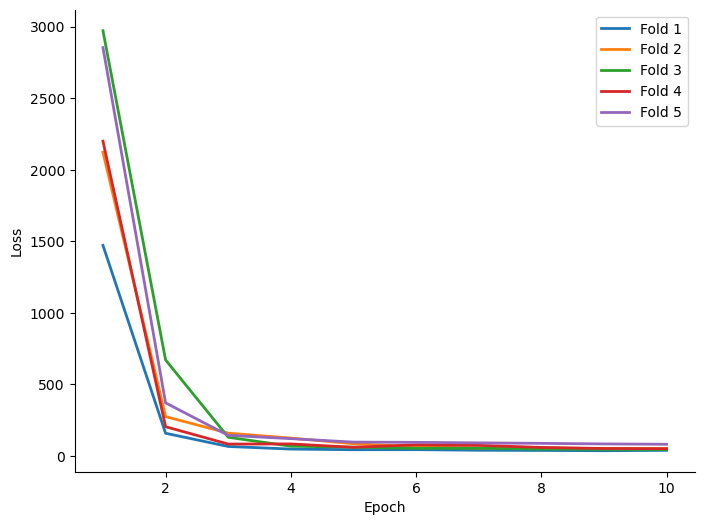
\includegraphics[width=\textwidth]{./ReportImages/train_loss_y2.png}
        \caption{\centering Training Loss for ETA \ac{KPI}}
        \label{fig:Training Loss for ETA grid}
    \end{minipage}
\end{figure}

\begin{figure}[H]
    \centering
    \begin{minipage}[b]{0.325\textwidth}
        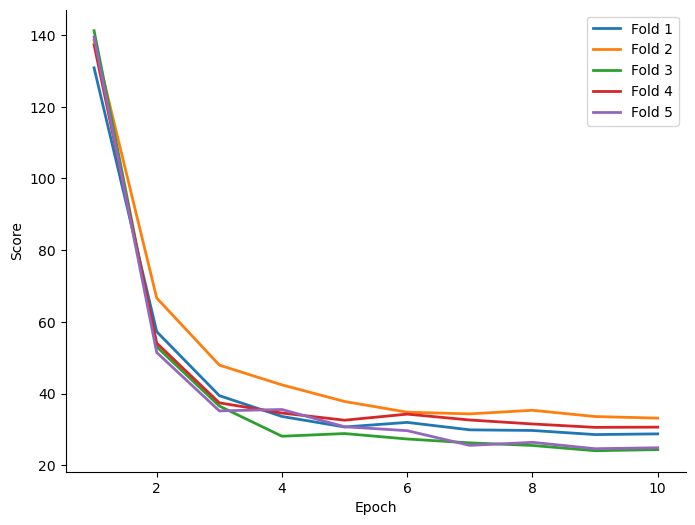
\includegraphics[width=\textwidth]{./ReportImages/train_score.png}
        \caption{\centering Aggregated Training Score}
        \label{fig:Aggregated Training Score}
    \end{minipage}
    \hfill
    \begin{minipage}[b]{0.325\textwidth}
        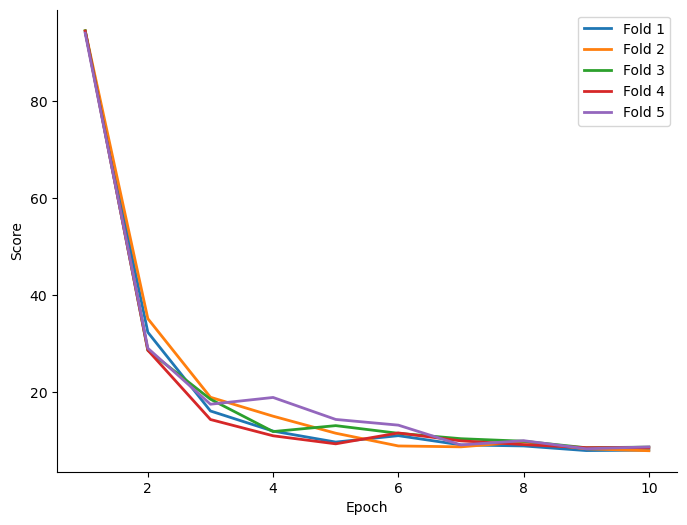
\includegraphics[width=\textwidth]{./ReportImages/train_score_y1.png}
        \caption{\centering Training Score for Mgrenz \ac{KPI}}
        \label{fig:Training Score for Torque Curve}
    \end{minipage}
    \hfill
    \begin{minipage}[b]{0.325\textwidth}
        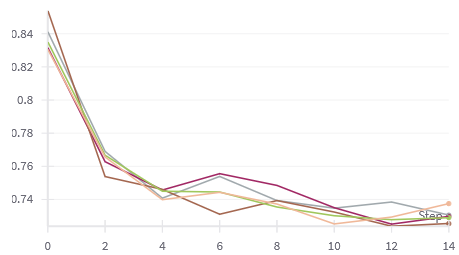
\includegraphics[width=\textwidth]{./ReportImages/train_score_y2.png}
        \caption{\centering Training Score for ETA \ac{KPI}}
        \label{fig:Training Score for ETA grid}
    \end{minipage}
\end{figure}

From the training plots we see that the model has converged after having run for 10 epochs.\\
Even though the weightage assigned to the ETA \ac{KPI} is significantly more in addition to loss regularization parameter, it seems to struggle to learn beyond a threshold and overfit by the 5th epoch.\\
We hypothesize to further increase the weightage of the ETA \ac{KPI}.
The Mgrenz \ac{KPI} shows promise in learning better but it would be at the cost of overfitting the ETA \ac{KPI}.\\
The Validations plots tells us the same tale although the ETA \ac{KPI} stops to learn after a certain point.

\begin{figure}[H]
    \centering
    \begin{minipage}[b]{0.325\textwidth}
        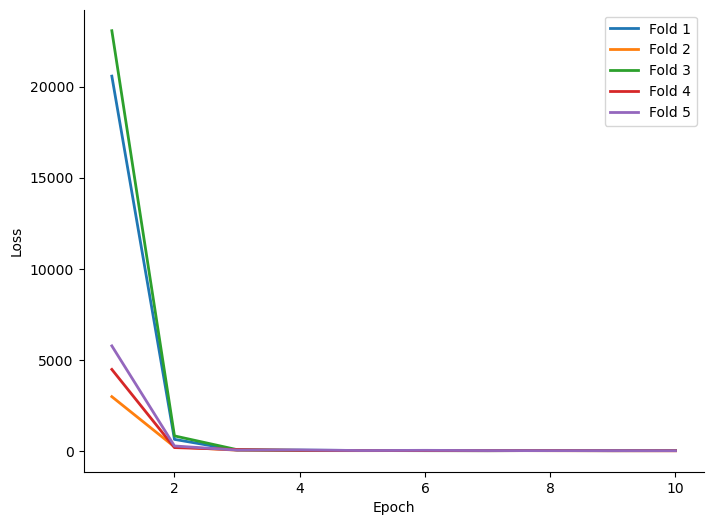
\includegraphics[width=\textwidth]{./ReportImages/val_loss.png}
        \caption{\centering Aggregated Validation Loss}
        \label{fig:Aggregated Validation Loss}
    \end{minipage}
    \begin{minipage}[b]{0.325\textwidth}
        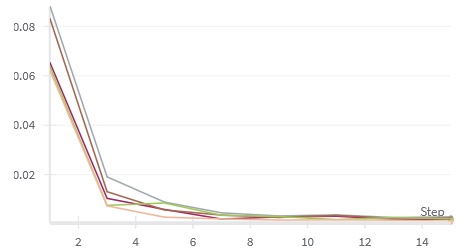
\includegraphics[width=\textwidth]{./ReportImages/val_loss_y1.png}
        \caption{\centering Validation Loss for Mgrenz \ac{KPI}}
        \label{fig:Validation Loss for Torque Curve}
    \end{minipage}
    \hfill
    \begin{minipage}[b]{0.325\textwidth}
        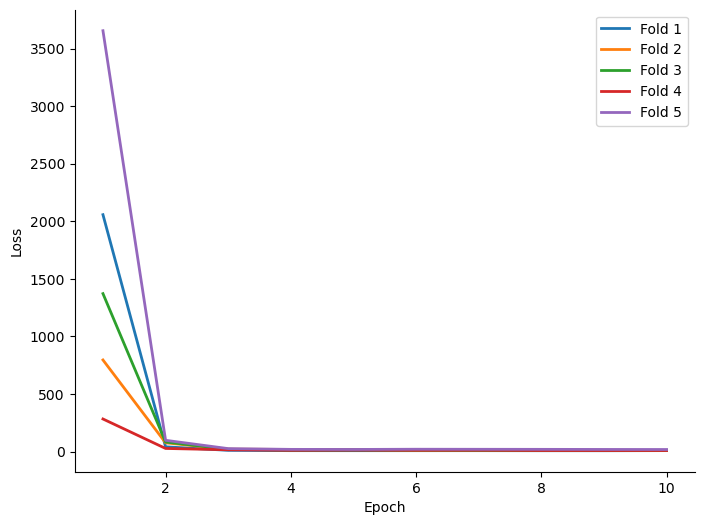
\includegraphics[width=\textwidth]{./ReportImages/val_loss_y2.png}
        \caption{\centering Validation Loss for ETA \ac{KPI}}
        \label{fig:Validation Loss for ETA grid}
    \end{minipage}
\end{figure}

\begin{figure}[H]
    \centering
    \begin{minipage}[b]{0.325\textwidth}
        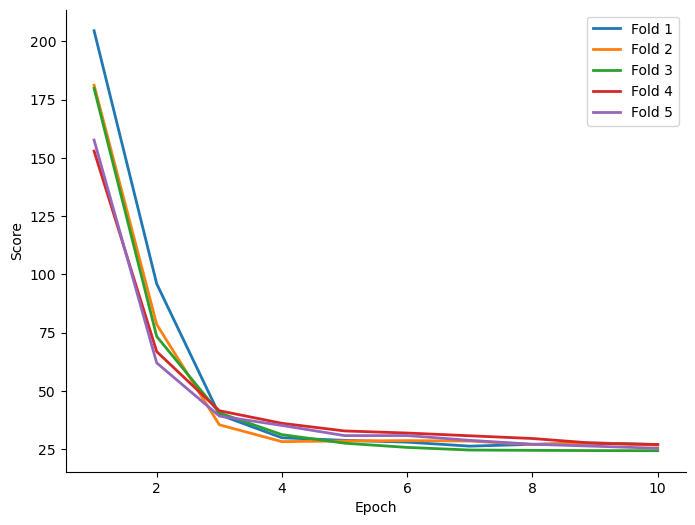
\includegraphics[width=\textwidth]{./ReportImages/val_score.png}
        \caption{\centering Aggregated Validation Score}
        \label{fig:Aggregated Validation Score}
    \end{minipage}
    \begin{minipage}[b]{0.325\textwidth}
        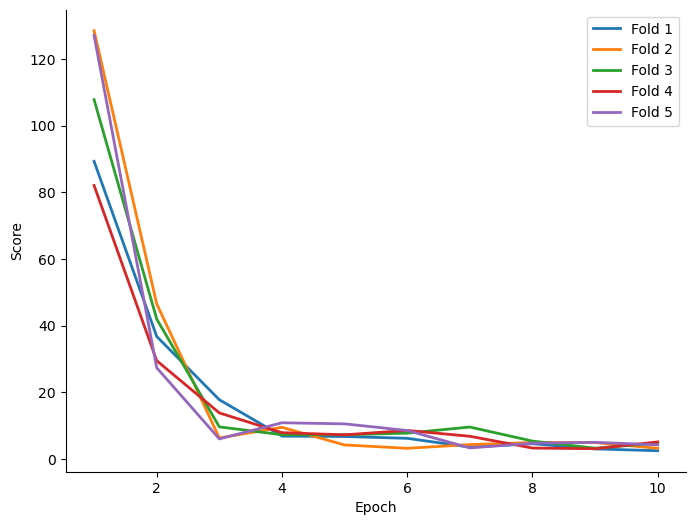
\includegraphics[width=\textwidth]{./ReportImages/val_score_y1.png}
        \caption{\centering Validation Score for Mgrenz \ac{KPI}}
        \label{fig:Validation Score for Torque Curve}
    \end{minipage}
    \hfill
    \begin{minipage}[b]{0.325\textwidth}
        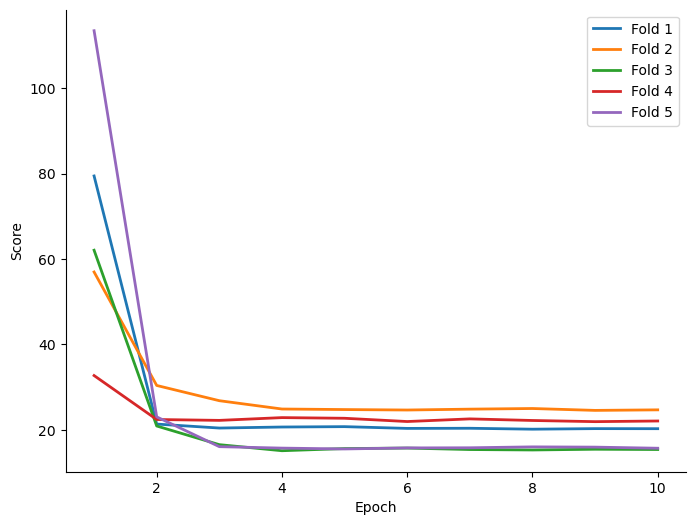
\includegraphics[width=\textwidth]{./ReportImages/val_score_y2.png}
        \caption{\centering Validation Score for ETA \ac{KPI}}
        \label{fig:Validation Score for ETA grid}
    \end{minipage}
\end{figure}

We have also enabled saving the best performant fold locally so it can be loaded on demand by the client when in need to only run inference.\\
We have narrowed down scoring to follow the criteria as depicted in Table \ref{tab:Scoring Criteria}.

\begin{table}[H]
    \centering
    \begin{tabularx}{1\linewidth}{|X|X|X|X|X|X|X|X|X|X|}
    \hline {\bf Percentage Difference} & {\bf 0-5\%} & {\bf 5-10\%} & {\bf 10-15\%} & {\bf 15-20\%} & {\bf 20-25\%} & {\bf 25-30\%} & {\bf 30-35\%} & {\bf 35-40\%} & {\bf 40-100\%}\\
    \hline 
    Y1 Score& 0-11& 11-22 & 22-33 & 33-44 & 44-55& 55-66 & 66-77 & 77-88 & \textgreater 88\\
    Y2 Score& 0-5 & 5-10 & 10-15 & 15-20 & 20-25& 25-30 & 30-35 & 35-40 &\textgreater 40\\
    \hline
    \end{tabularx}
    \caption{Scoring Criteria}
    \label{tab:Scoring Criteria}
\end{table}

This is deduced from the Equation \ref{eq:Percentage Difference}
\begin{equation}
    \text{Percentage Difference} = (\text{Score} / {(Max - Min)})  \times 100
    \label{eq:Percentage Difference}
\end{equation}

From our observations the target values for Mgrenz \ac{KPI} range between 50-280 and those of the ETA \ac{KPI} range between 0-100.

\section{Results with \ac{MLP}}\label{sec:Results with MLP}

\subsection{Mgrenz \ac{KPI} Results with \ac{MLP}}\label{sec:2D Torque Curve Results with MLP}

\begin{figure}[H]
    \centering
    \includegraphics[width=1\textwidth]{./ReportImages/KPI2D_predictions.png} 
    \caption{MLP Training Results for Mgrenz \ac{KPI}} 
    \label{fig:MLP Training Results for 2D KPI(Mgrenz)}
\end{figure}

Figure \ref{fig:MLP Training Results for 2D KPI(Mgrenz)} depicts the difference and percentage difference on a twin scale to give a rough overview of the prediction deviations from the targets.
Whereas the \ac{RMSE} equivalent to the Y1 score tells us that for 50\% of the plots shown, the predictions are off by about 5\% from the target values as per Table \ref{tab:Scoring Criteria}.\\
Figure \ref{fig:MLP RMSE Evaluation for 2D KPI(Mgrenz)} shows us the Average \ac{RMSE} and element wise \ac{RMSE} for the test dataset performance with the \ac{MLP}. \\
Our inferences are overall the predictions closely resemble the trajectory of the target values allthough they fluctuate.
Experimenting with the hyperparameters \textit{lambda1\_y1} and \textit{lambda2\_y1} has potential to improve this anomaly. 
In addition granting a higher weight \textit{wt} can also help in this direction.\\
\begin{figure}[H]
    \centering
    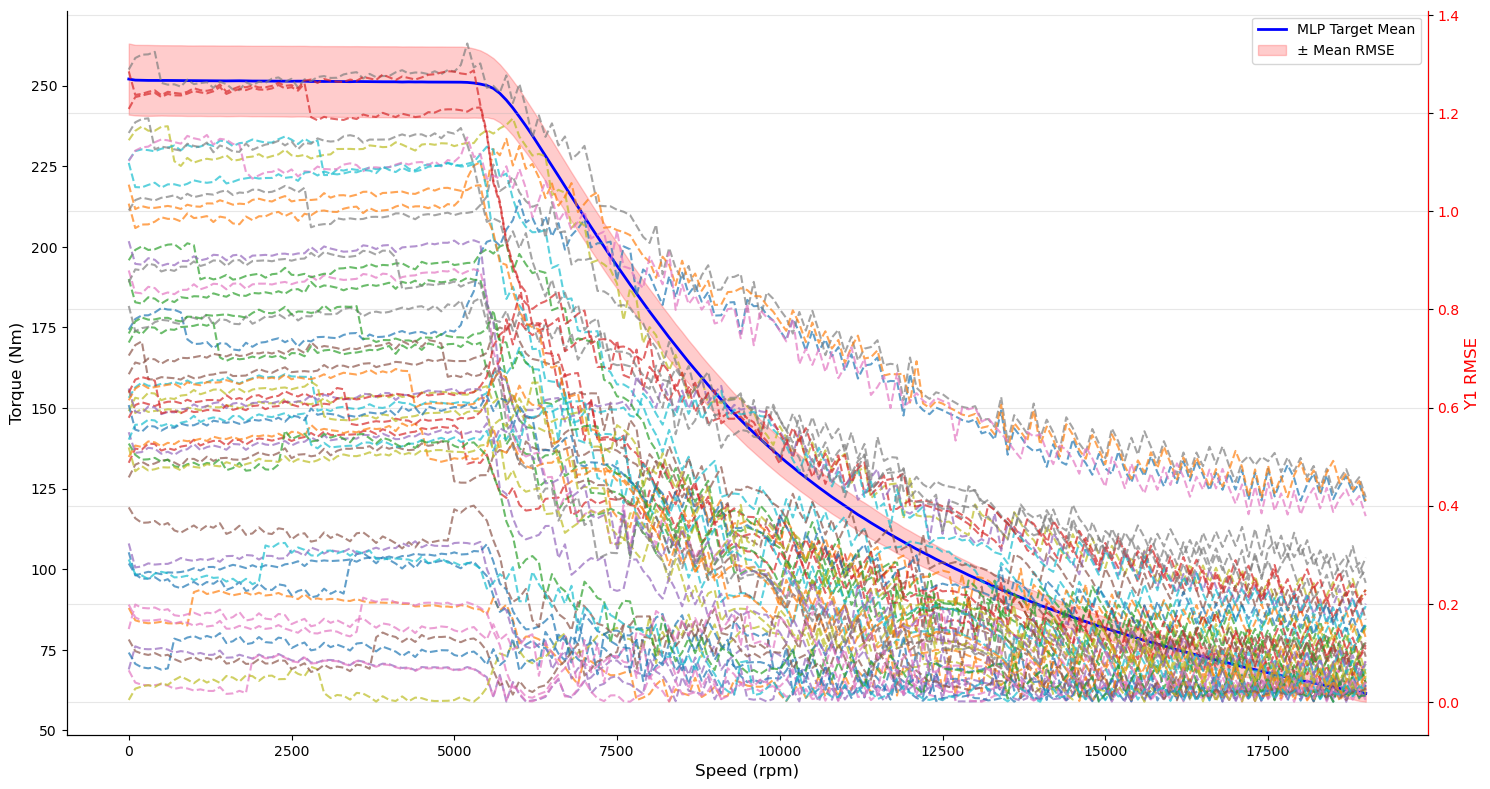
\includegraphics[width=1\textwidth]{./ReportImages/RMSE_MLP_y1.png} 
    \caption{\ac{MLP} \ac{RMSE} Evaluation for Mgrenz \ac{KPI}} 
    \label{fig:MLP RMSE Evaluation for 2D KPI(Mgrenz)}
\end{figure}


Figure \ref{fig:MLP Score statistics for 2D KPI(Mgrenz)} shows the score statistics of the model performance of Mgrenz \ac{KPI} over the entire test dataset.
The Y1 \ac{RMSE} from Equation \ref{eq:Y1 Score} is calculated for each sample and shown as a histogram.\\

\begin{figure}[H]
    \centering
    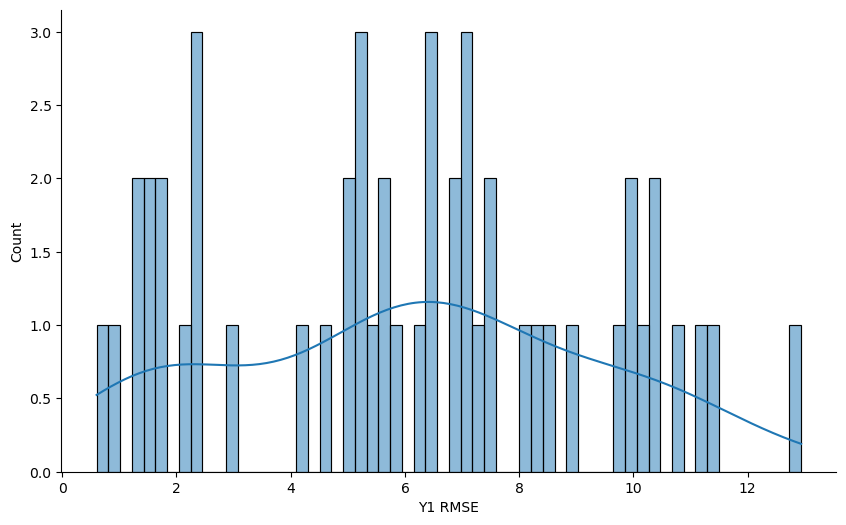
\includegraphics[width=0.8\textwidth]{./ReportImages/score_MLP_y1.png } 
    \caption{MLP Score statistics for Mgrenz \ac{KPI}} 
    \label{fig:MLP Score statistics for 2D KPI(Mgrenz)}
\end{figure}
It also tells us that the \ac{RMSE}s are almost evenly distributed between 0.5-12.5 thus encompassing a range of 0-6\% difference with the target values.\\

\subsection{ETA \ac{KPI} Results with \ac{MLP}}\label{sec:3D ETA Grid Results with MLP}

The results of the \ac{MLP} model from inference with its corresponding overlap is shown below: \\

\begin{figure}[H]
    \centering
    \includegraphics[width=1\textwidth]{./ReportImages/KPI3Dprediction1.png} 
    \caption{1st MLP Training Results for ETA \ac{KPI}} 
    \label{fig:1st MLP Training Results for 3D KPI(ETA)}
\end{figure}

\begin{figure}[H]
    \centering
    \includegraphics[width=1\textwidth]{./ReportImages/evalKPI3Dprediction1.png} 
    \caption{1st Eval MLP Training Results for ETA \ac{KPI}} 
    \label{fig:1st Eval MLP Training Results for 3D KPI(ETA)}
\end{figure}

From a visual perspective, the predictions to relative extent resembles the target and the regularization of the ETA \ac{KPI} seems to be already teaching the model that the envelope should follow the Mgrenz \ac{KPI} curve shape.  
The curve being sliced off irregularly is the effect of us trying to retain the Mgrenz \ac{KPI} shape as was discussed in Section \ref{sec:Post Processing}.\\
This could be having negative impacts for the ETA \ac{KPI}  when the predictions for the Mgrenz \ac{KPI} are not perfect.
This is yet again a decision to be made based on which of the 2 targets to prioritize. \\

Moreover we calculate the RMSE and differences of prediction from the target by truncating the matrices to be of common shape.
We also replace \ac{NaN} values with 0 in either if it occurs as the ETA \ac{KPI}'s were padded with \ac{NaN}'s to be of the same shape but originally had no values as was discussed in Section \ref{sec:Deep Dive into 3D KPI}.\\

\begin{figure}[H]
    \centering
    \includegraphics[width=1\textwidth]{./ReportImages/KPI3Dprediction2.png} 
    \caption{2nd MLP Training Results for ETA \ac{KPI}} 
    \label{fig:2nd MLP Training Results for 3D KPI(ETA)}
\end{figure}


\begin{figure}[H]
    \centering
    \includegraphics[width=1\textwidth]{./ReportImages/evalKPI3Dprediction2.png} 
    \caption{2nd Eval MLP Training Results for ETA \ac{KPI}} 
    \label{fig:2nd Eval MLP Training for 3D KPI(ETA)}
\end{figure}

\begin{figure}[H]
    \centering
    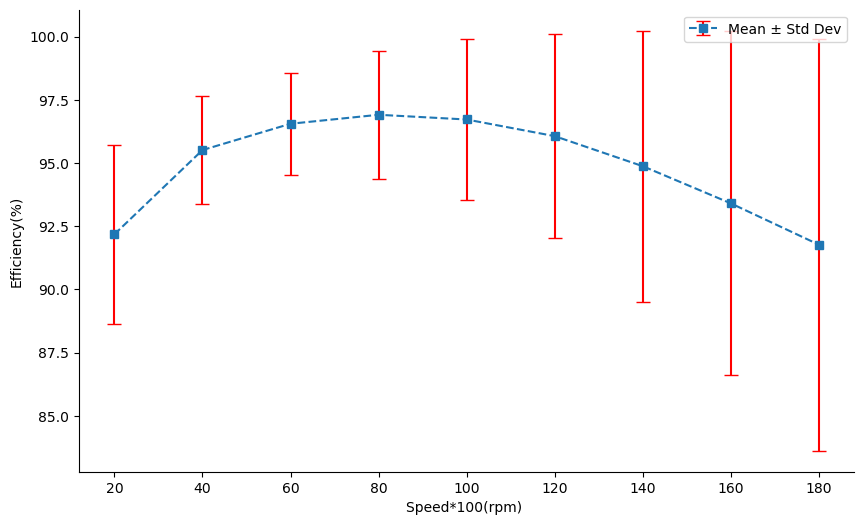
\includegraphics[width=0.8\textwidth]{./ReportImages/stddev_y2_nn_MLP.png} 
    \caption{\ac{MLP} Standard Deviation of ETA \ac{KPI} Positive Grid across Speed Intervals} 
    \label{fig:MLP Standard Deviation of 3D KPI(ETA) Positive Grid across Speed Intervals}
\end{figure}

Figure \ref{fig:MLP Standard Deviation of 3D KPI(ETA) Positive Grid across Speed Intervals} shows the standard deviation across different speed ranges for the \ac{MLP} predictions.
In comparisions to Figure \ref{fig:Standard Deviation of 3D KPI(ETA) Positive Grid across Speed Intervals} we infer that as the speed increases the target deviations of efficiency values are not so accurately captured by the model.

ETA \ac{KPI} is harder to evaluate scoring as it is a \ac{3D} plot. 
Therefore, to visualize the Efficiency prediction deviation with its respective targets we do so for specific speeds across the entire torque range with Figure \ref{fig:Eval MLP ETA RMSE KPI}.
The speeds are chosen at equal intervals of 2000 rpm.\\
We can observe that the most deviation occurs towards the higher torque values for each corresponding speed. In layman terms, this would be towards the ETA envelope tapering off.\\
This anomaly can be explained by the Mgrenz \ac{KPI} predictions not being up to mark as it is responsible for trimming the edges of the envelope.\\
However it is not only the border of the envelope a question of concern here but also for neigbouring values of the envelope specifically from 1/4 the speed onwards.
The reason why it deteroirates from 1/4 the speed onwards is because the ETA \ac{KPI}'s envelope starts to converge from around 6000 rpm as we can see in Figure \ref{fig:Efficiency Grid}\\
We remedied it to a impressive extent by increasing the parameter \textit{t2}.
Nevertheless, we see on average among the speeds, the \ac{RMSE} is close to 5 which is 5\% deviation from the target values as per Table \ref{tab:Scoring Criteria}.\\

Observations from the predictions helped to correct few discrepancies in our development for instance in the ETA grid we replaced 0 with \ac{NaN} values which we later understood were both represented different in the grid.\\
As Efficiency values can take up values only between 0-100, we consider the same as constant across plots and use it as a baseline for determining the levels in the contour plot. \\ 
We have also left the output predictions for the Torque curve to remain as float values even when the target values are integers to preserve data precision. We give the client the flexibility to turn this on/off demand. \\

\begin{figure}[H]
    \centering
    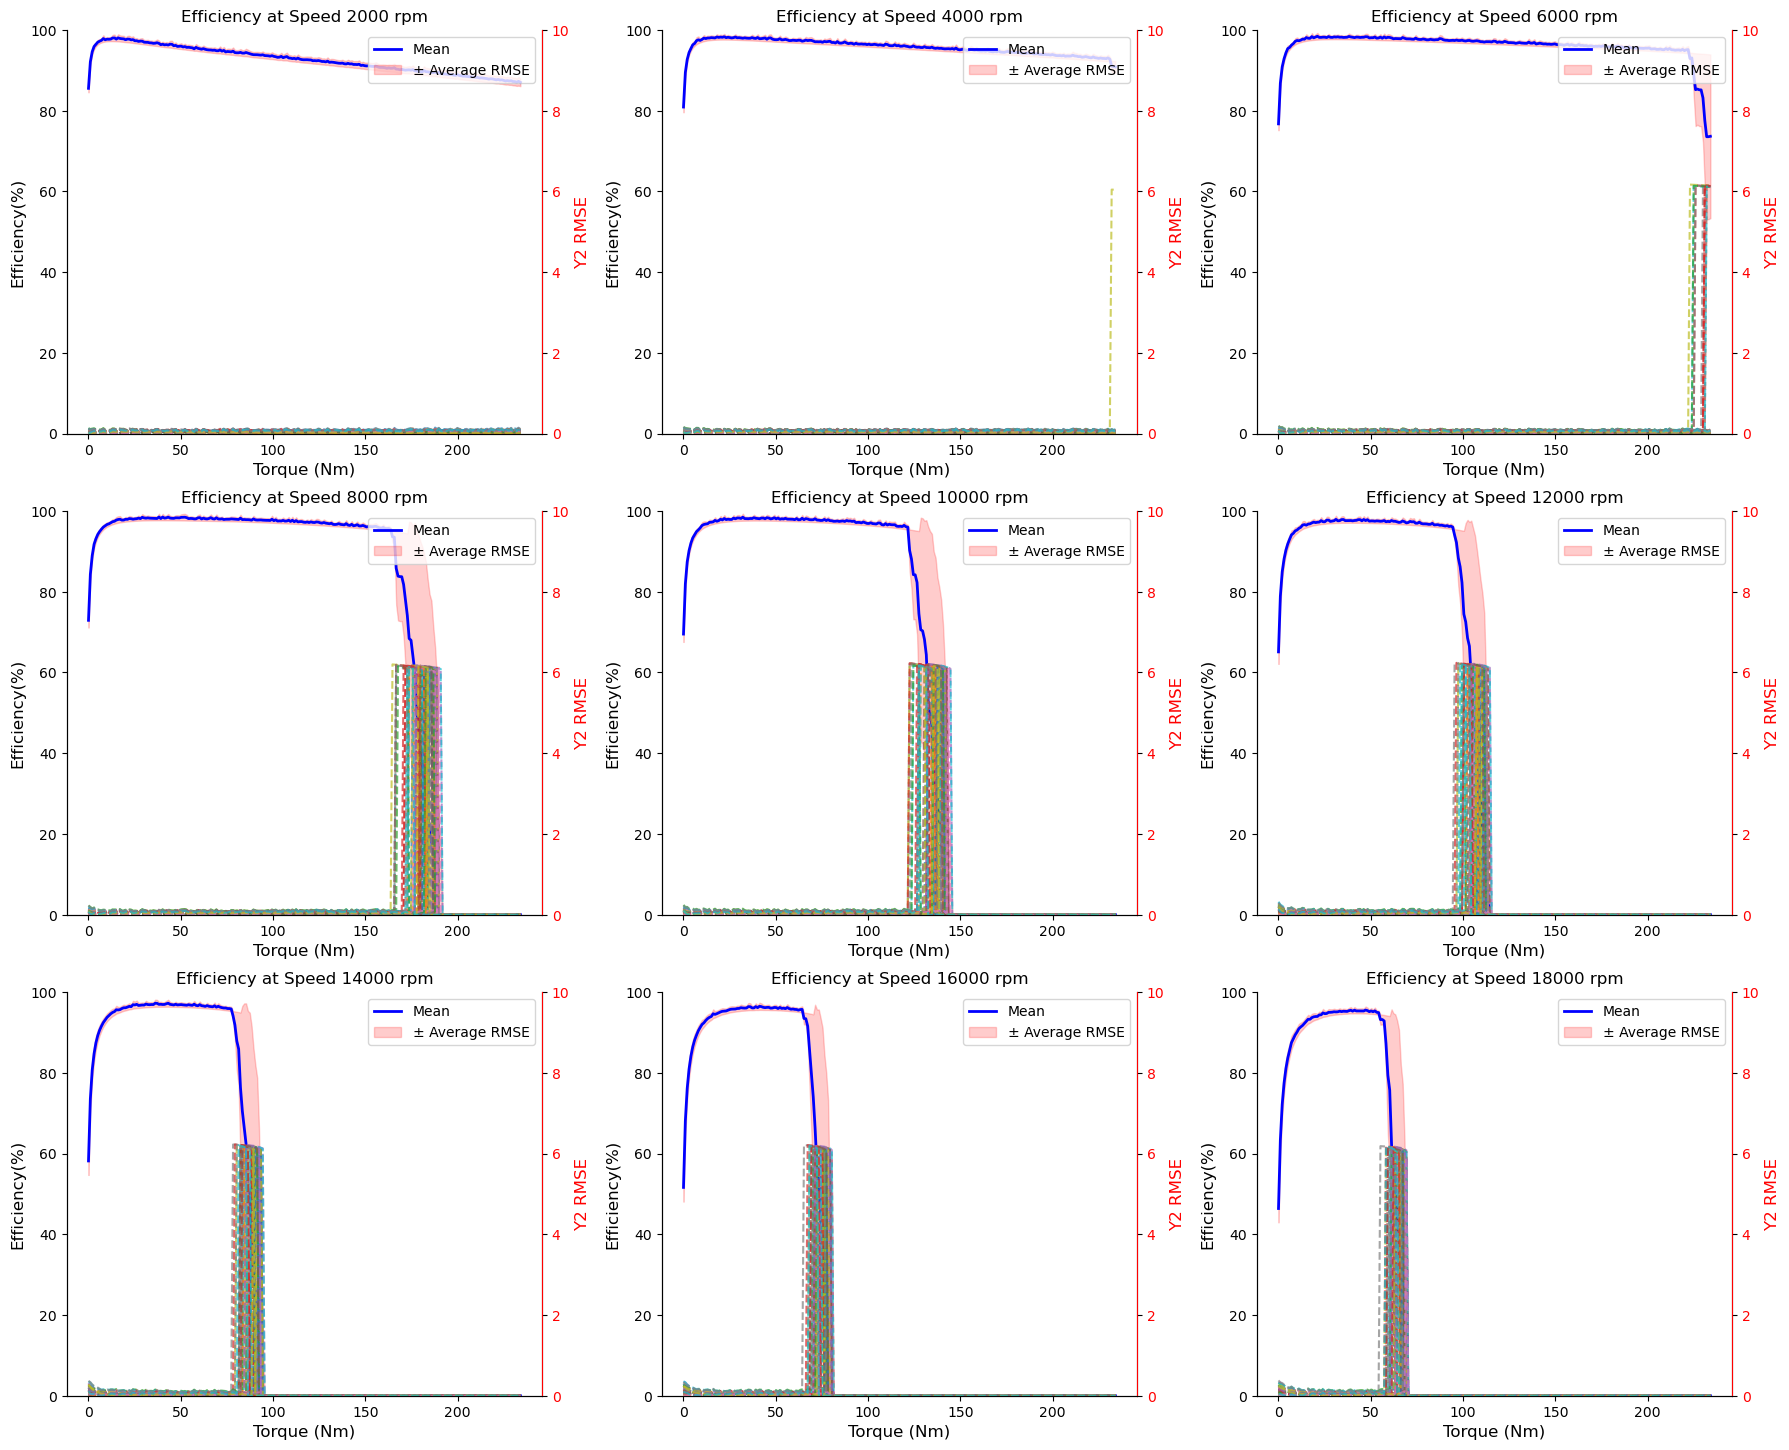
\includegraphics[width=1\textwidth]{./ReportImages/rmse_eta_MLP.png} 
    \caption{Eval MLP ETA \ac{RMSE} \ac{KPI}} 
    \label{fig:Eval MLP ETA RMSE KPI}
\end{figure}

Figure \ref{fig:MLP Score statistics for 3D KPI(ETA)} shows the score statistics of the model performance of ETA \ac{KPI} over the test dataset.
The Y2 \ac{RMSE} from Equation \ref{eq:Y2 Score} is calculated for each sample and shown as a histogram.\\
On an average the \ac{RMSE} is close to 13, which is 13\% deviation from the target values as per Table \ref{tab:Scoring Criteria}.\\

\begin{figure}[H]
    \centering
    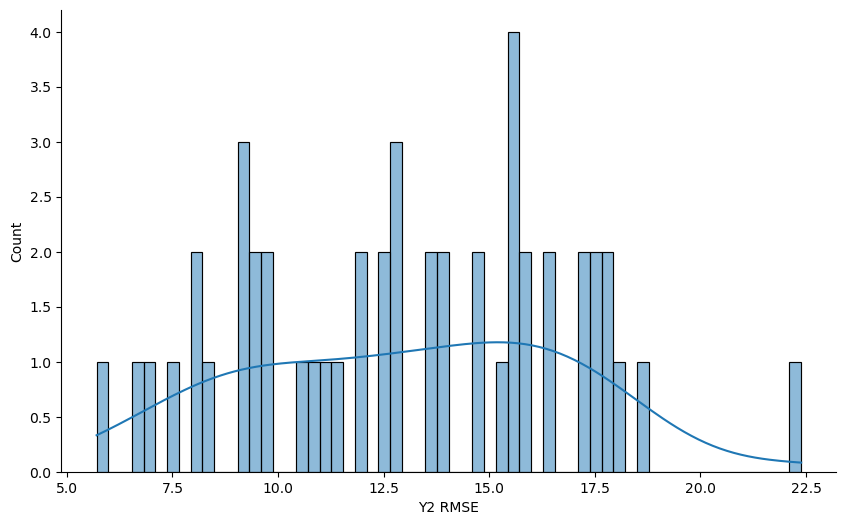
\includegraphics[width=0.8\textwidth]{./ReportImages/score_MLP_y2.png } 
    \caption{MLP Score statistics for ETA \ac{KPI}} 
    \label{fig:MLP Score statistics for 3D KPI(ETA)}
\end{figure}

\section{Results with Baseline}\label{sec:Results with Baseline}

From our observations on how the predictions closely resembled that of the target values in Section \ref{sec:Data Preprocessing for MLP}, we have developed a Baseline model which is essentially the average of the train dataset.

\subsection{Mgrenz \ac{KPI} Results with Baseline}\label{sec:3D ETA Grid Results with Baseline}

The Y1 Baseline score for the ETA \ac{KPI} is formulated in Equation \ref{eq:Y1 Baseline Score} :

\begin{equation}
    \text{Y1 Baseline Score} = \frac{1}{n} \sum_{i=1}^{n} \underbrace{ \sqrt{\frac{1}{h} \sum_{j=1}^{h} (\bar{y} - y_{ij})^2}}_{Y1\ Baseline\ RMSE}
    \label{eq:Y1 Baseline Score}
    \end{equation}
    
    \makebox[\textwidth][c]{%
        \begin{minipage}{0.55\textwidth}
            \centering
            \textit{where
                    \begin{itemize}
                        \item $\bar{y}$  : Baseline Average mean
                        \item h : Columns of 1D vector
                        \item Y1 Baseline \ac{RMSE}: \ac{RMSE} for each test sample
                    \end{itemize}
                    }
        \end{minipage}
    }
    

\vspace{1em} % Adjust the space here, e.g., 1em or 2em

Figure \ref{fig:Baseline RMSE Evaluation for 2D KPI(Mgrenz)} shows the Average \ac{RMSE} and element wise \ac{RMSE} for the test dataset performance with the Baseline Model.\\

\begin{figure}[H]
    \centering
    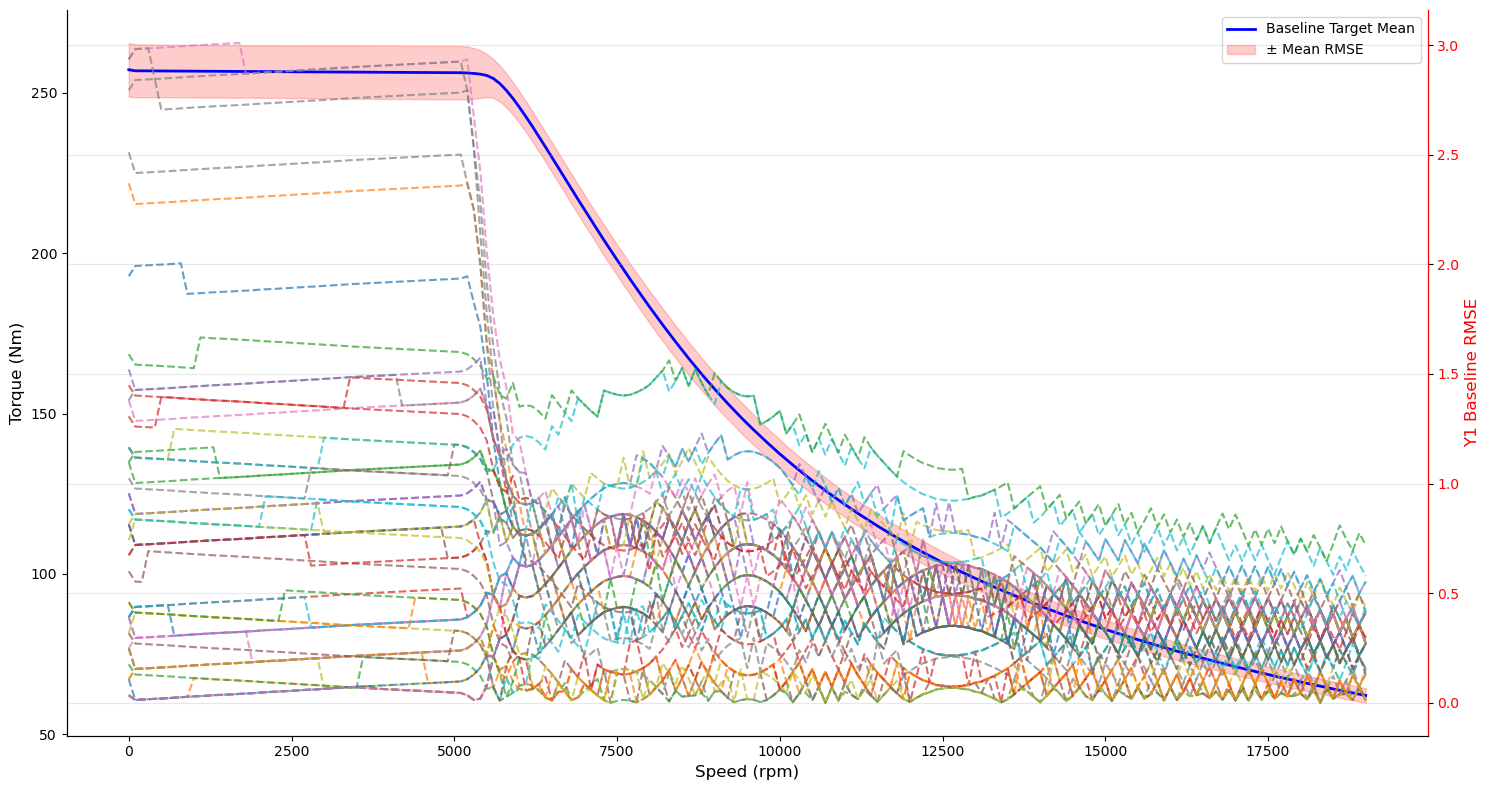
\includegraphics[width=1\textwidth]{./ReportImages/RMSE_Baseline_y1.png} 
    \caption{Baseline \ac{RMSE} Evaluation for 2D KPI(Mgrenz)} 
    \label{fig:Baseline RMSE Evaluation for 2D KPI(Mgrenz)}
\end{figure}

We can see that the deviations are at its most towards the beginning of the curve. 
We also observe that there are no fluctuations in the curve as compared to the Predictions.\\

\subsection{ETA \ac{KPI} Results with Baseline}\label{sec:3D ETA Grid Results with Baseline}

The Y2 Baseline score for the ETA \ac{KPI} is formulated in Equation \ref{eq:Y2 Baseline Score} :
%  Evaluation metric (\ac{MSE}) Loss for 3D KPI
\begin{equation}
    \text{Y2 Baseline Score} = \frac{1}{n} \sum_{i=1}^{n} \underbrace{ \sqrt{\frac{1}{w} \frac{1}{h} \sum_{j=1}^{w} \sum_{k=1}^{h} (\bar{y} - y_{ijk})^2}}_{Y2\ Baseline\ RMSE}
    \label{eq:Y2 Baseline Score}
\end{equation}
    

\makebox[\textwidth][c]{%
    \begin{minipage}{0.55\textwidth}
        \centering
        \textit{where
                \begin{itemize}
                    \item w : Rows of 2D vector
                    \item h : Columns of 2D vector
                    \item Y2 Baseline \ac{RMSE} : \ac{RMSE} for each test sample
                \end{itemize}
                }
    \end{minipage}
}

\vspace{1em} % Adjusts vertical space between equation and text

Figure \ref{fig:Eval Baseline ETA RMSE KPI} gives a neat visualization of the Baseline Efficiency \ac{RMSE} with its respective targets for specific speeds across the entire torque range.
The speeds are chosen at equal intervals of 2000 rpm.\\
We infer from the plots that the targets have essentially the same values across the entire grid.\\
We arrive at this conclusion from the fact that the only region where we see significant deviation is at the ETA \ac{KPI} envelope and we attribute this pattern to stem from the corresponding Mgrenz \ac{KPI}'s curve. \\
Thus, the efficiency values are almost the same for more than 3/4th of the grid across all samples.\\
\begin{figure}[H]
    \centering
    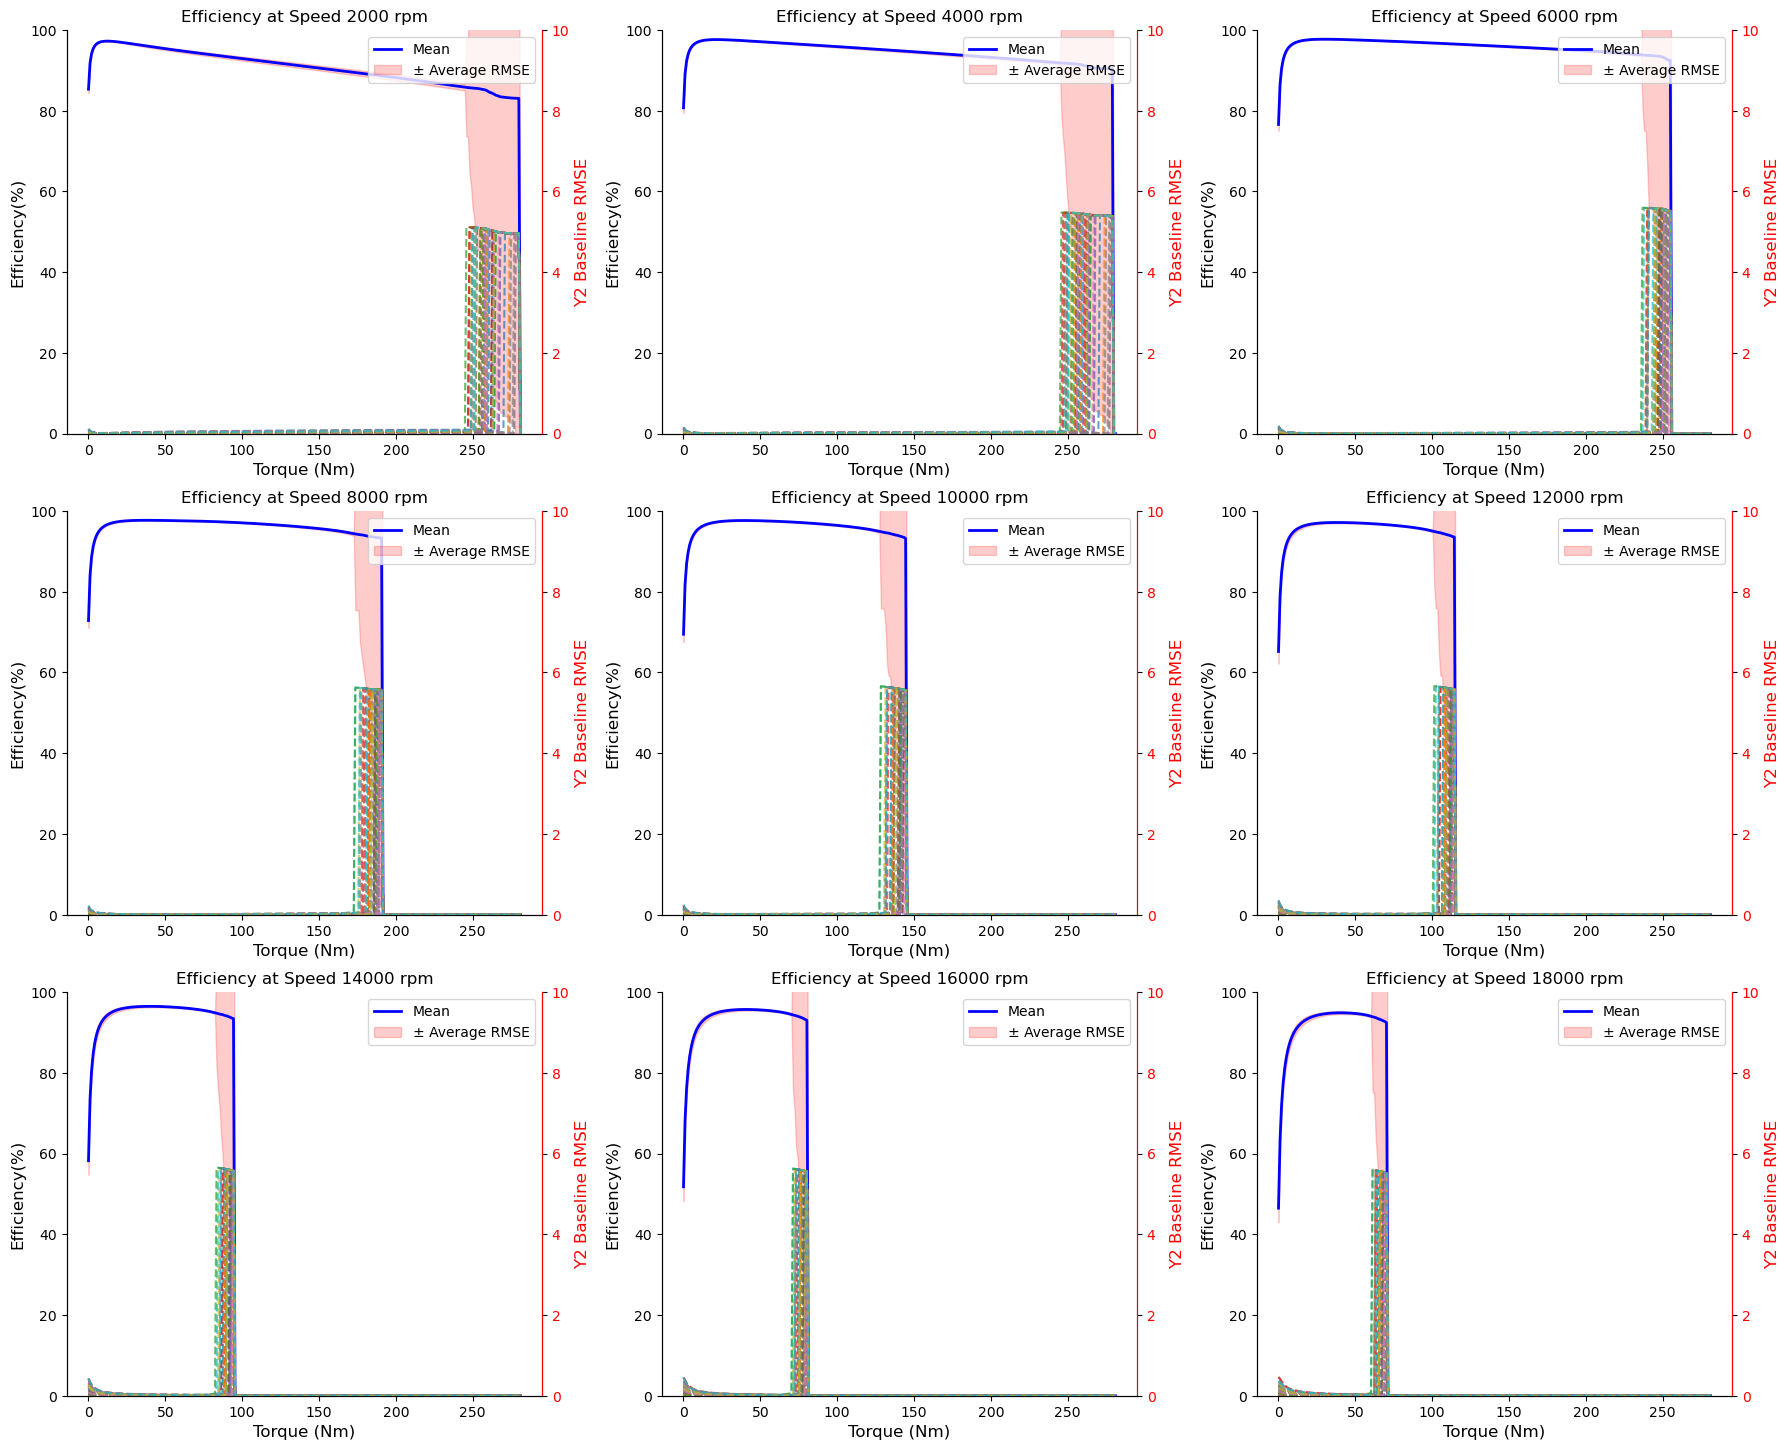
\includegraphics[width=1\textwidth]{./ReportImages/rmse_eta_Baseline.png} 
    \caption{Eval Baseline ETA \ac{RMSE} \ac{KPI}} 
    \label{fig:Eval Baseline ETA RMSE KPI}
\end{figure}

\section{Results with Smoothening Loss Regularization}\label{sec:Results with Smoothening Loss Regularization}

\subsection{Mgrenz \ac{KPI} Results with Smoothening Loss Regularization}\label{subsec:2D Mgrenz Results with Smoothening Loss Regularization}

Figure \ref{fig:Smoothening Mgrenz RMSE Evaluation for 2D KPI(Mgrenz)} shows the Average \ac{RMSE} and element wise \ac{RMSE} for the test dataset performance with the MLP Model with Smoothening Curve regularization discussed in Equation \ref{eq:Y1 Smoothening Loss Regularization}.\\

\begin{figure}[H]
    \centering
    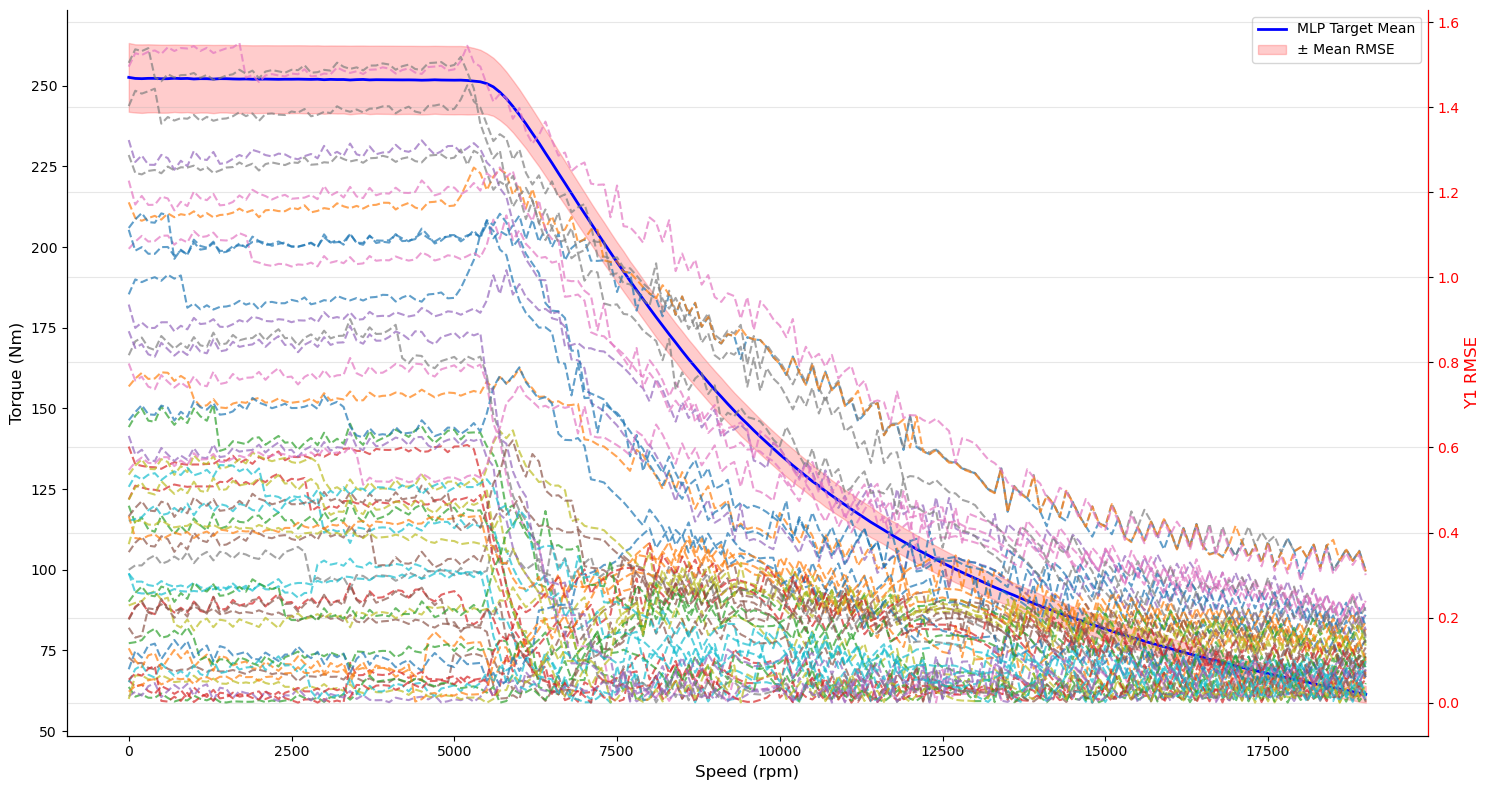
\includegraphics[width=1\textwidth]{./ReportImages/RMSE_MLP_Smoothening_y1.png} 
    \caption{Smoothening Mgrenz \ac{RMSE} Evaluation for 2D KPI(Mgrenz)} 
    \label{fig:Smoothening Mgrenz RMSE Evaluation for 2D KPI(Mgrenz)}
\end{figure}

We can see that the deviations are at its peak towards the beginning of the curve. 
We also observe that there are are fluctuations in the curve but relatively less when compared to Figure \ref{fig:MLP RMSE Evaluation for 2D KPI(Mgrenz)}\\

% \subsection{ETA \ac{KPI} Results with Smoothening Loss Regularization}\label{subsec:3D ETA Results with Smoothening Loss Regularization}

% Figure \ref{fig:Eval Baseline ETA RMSE KPI} gives a neat visualization of the Efficiency \ac{RMSE} with its respective targets for specific speeds across the entire torque range.
% The speeds are chosen at equal intervals of 2000 rpm.\\
% This figure is very much similar to the ones predicted with the \ac{MLP} model ea
% \begin{figure}[H]
%     \centering
%     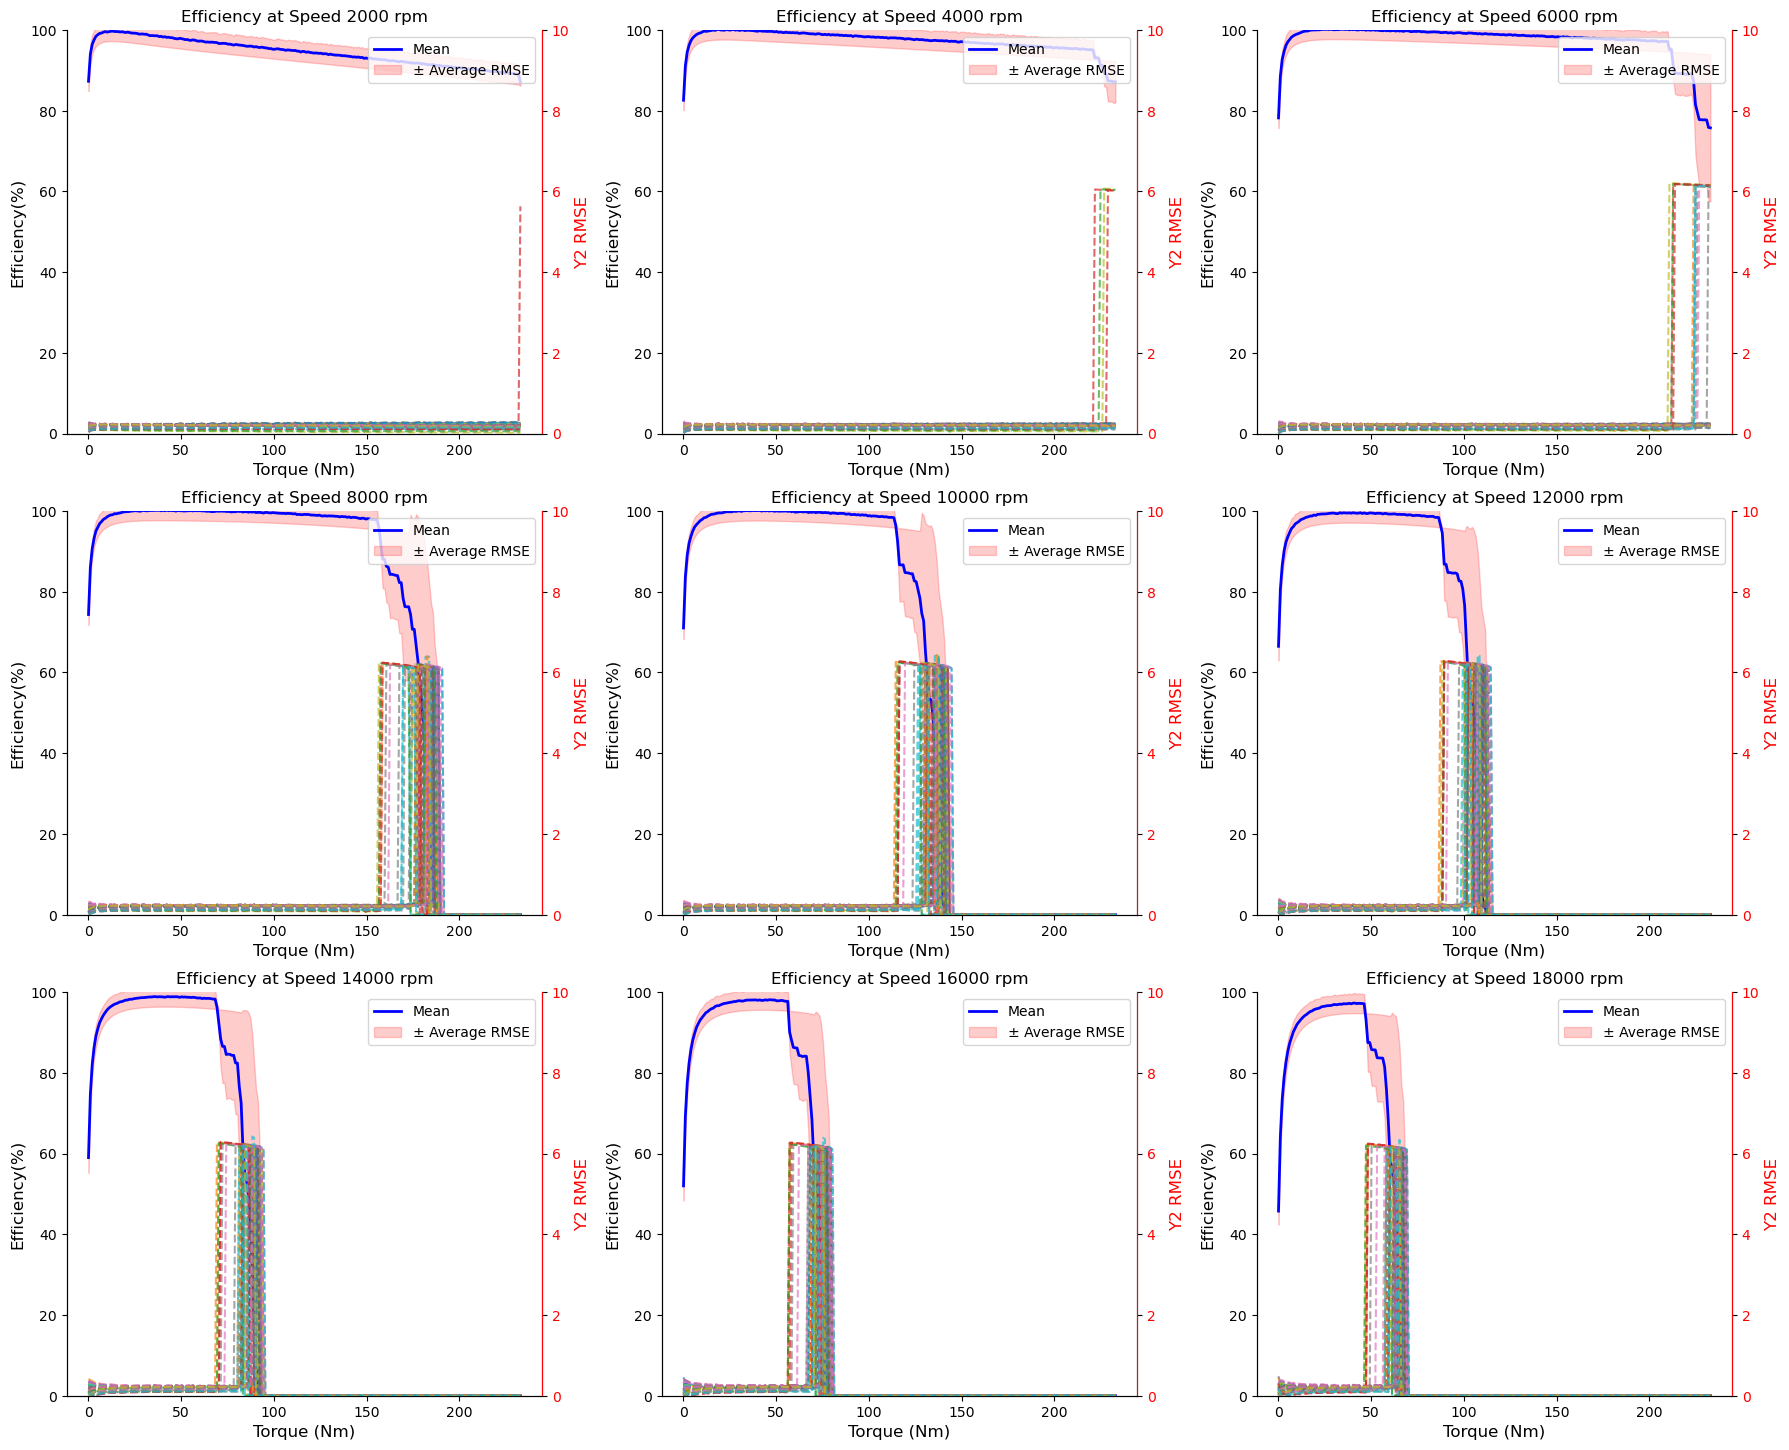
\includegraphics[width=1\textwidth]{./ReportImages/rmse_eta_Smoothening_MLP.png} 
%     \caption{Eval Smoothening Mgrenz \ac{RMSE} \ac{KPI}} 
%     \label{fig:Eval Smoothening Mgrenz RMSE KPI}
% \end{figure}

\section{Results with No Loss Regularization}\label{sec:Results with No Loss Regularization}

\subsection{Mgrenz \ac{KPI} Results with No Loss Regularization}\label{subsec:2D Mgrenz Results with No Loss Regularization}

Figure \ref{fig:0 Loss Regularization RMSE Evaluation for 2D KPI(Mgrenz)} shows the Average \ac{RMSE} and element wise \ac{RMSE} for the test dataset performance with the MLP Model without any regularizations.\\

\begin{figure}[H]
    \centering
    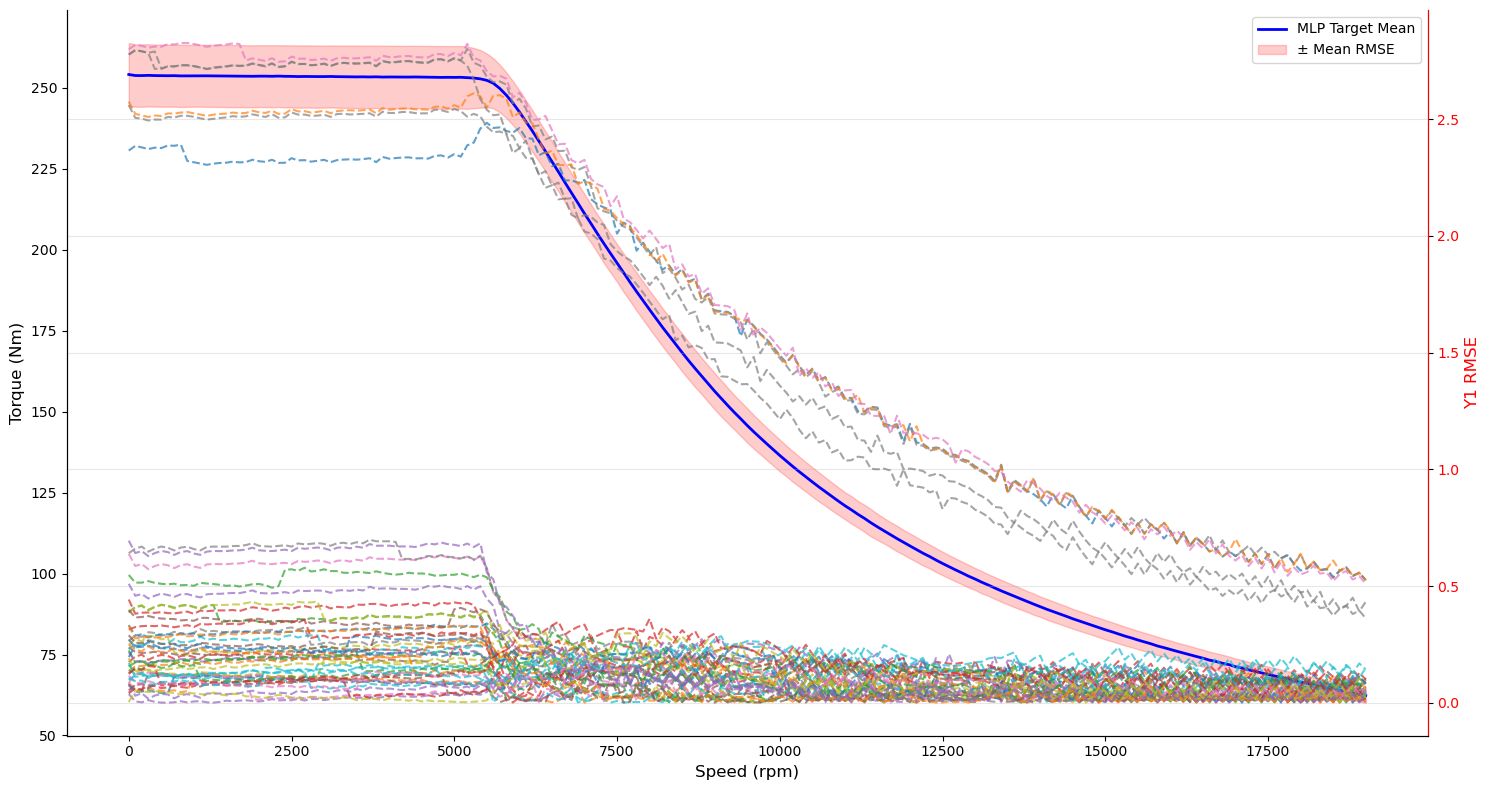
\includegraphics[width=1\textwidth]{./ReportImages/RMSE_MLP_no_lossreg_y1.png} 
    \caption{0 Loss Regularization \ac{RMSE} Evaluation for 2D KPI(Mgrenz)} 
    \label{fig:0 Loss Regularization RMSE Evaluation for 2D KPI(Mgrenz)}
\end{figure}

We can see that the deviations are at its peak towards the beginning of the curve however the \ac{RMSE} for most samples is close to negligible.
We also note there are fewer fluctuations in the curve as compared to the Predictions with Loss Regularizations.
This conclusion prompts us to omit the loss regularization for the Mgrenz \ac{KPI}'s.\\

\subsection{ETA \ac{KPI} Results with No Loss Regularization}\label{subsec:3D ETA Results with No Loss Regularization}

Figure \ref{fig:Eval 0 Loss Regularization ETA RMSE KPI} gives a neat visualization of the Baseline Efficiency \ac{RMSE} with its respective targets for specific speeds across the entire torque range.
The speeds are chosen at equal intervals of 2000 rpm.\\
We infer from the plots that they are very similar to the ones generated with loss regularization in place
This fuels us to also omit the loss regularizations for the ETA \ac{KPI}'s.\\
\begin{figure}[H]
    \centering
    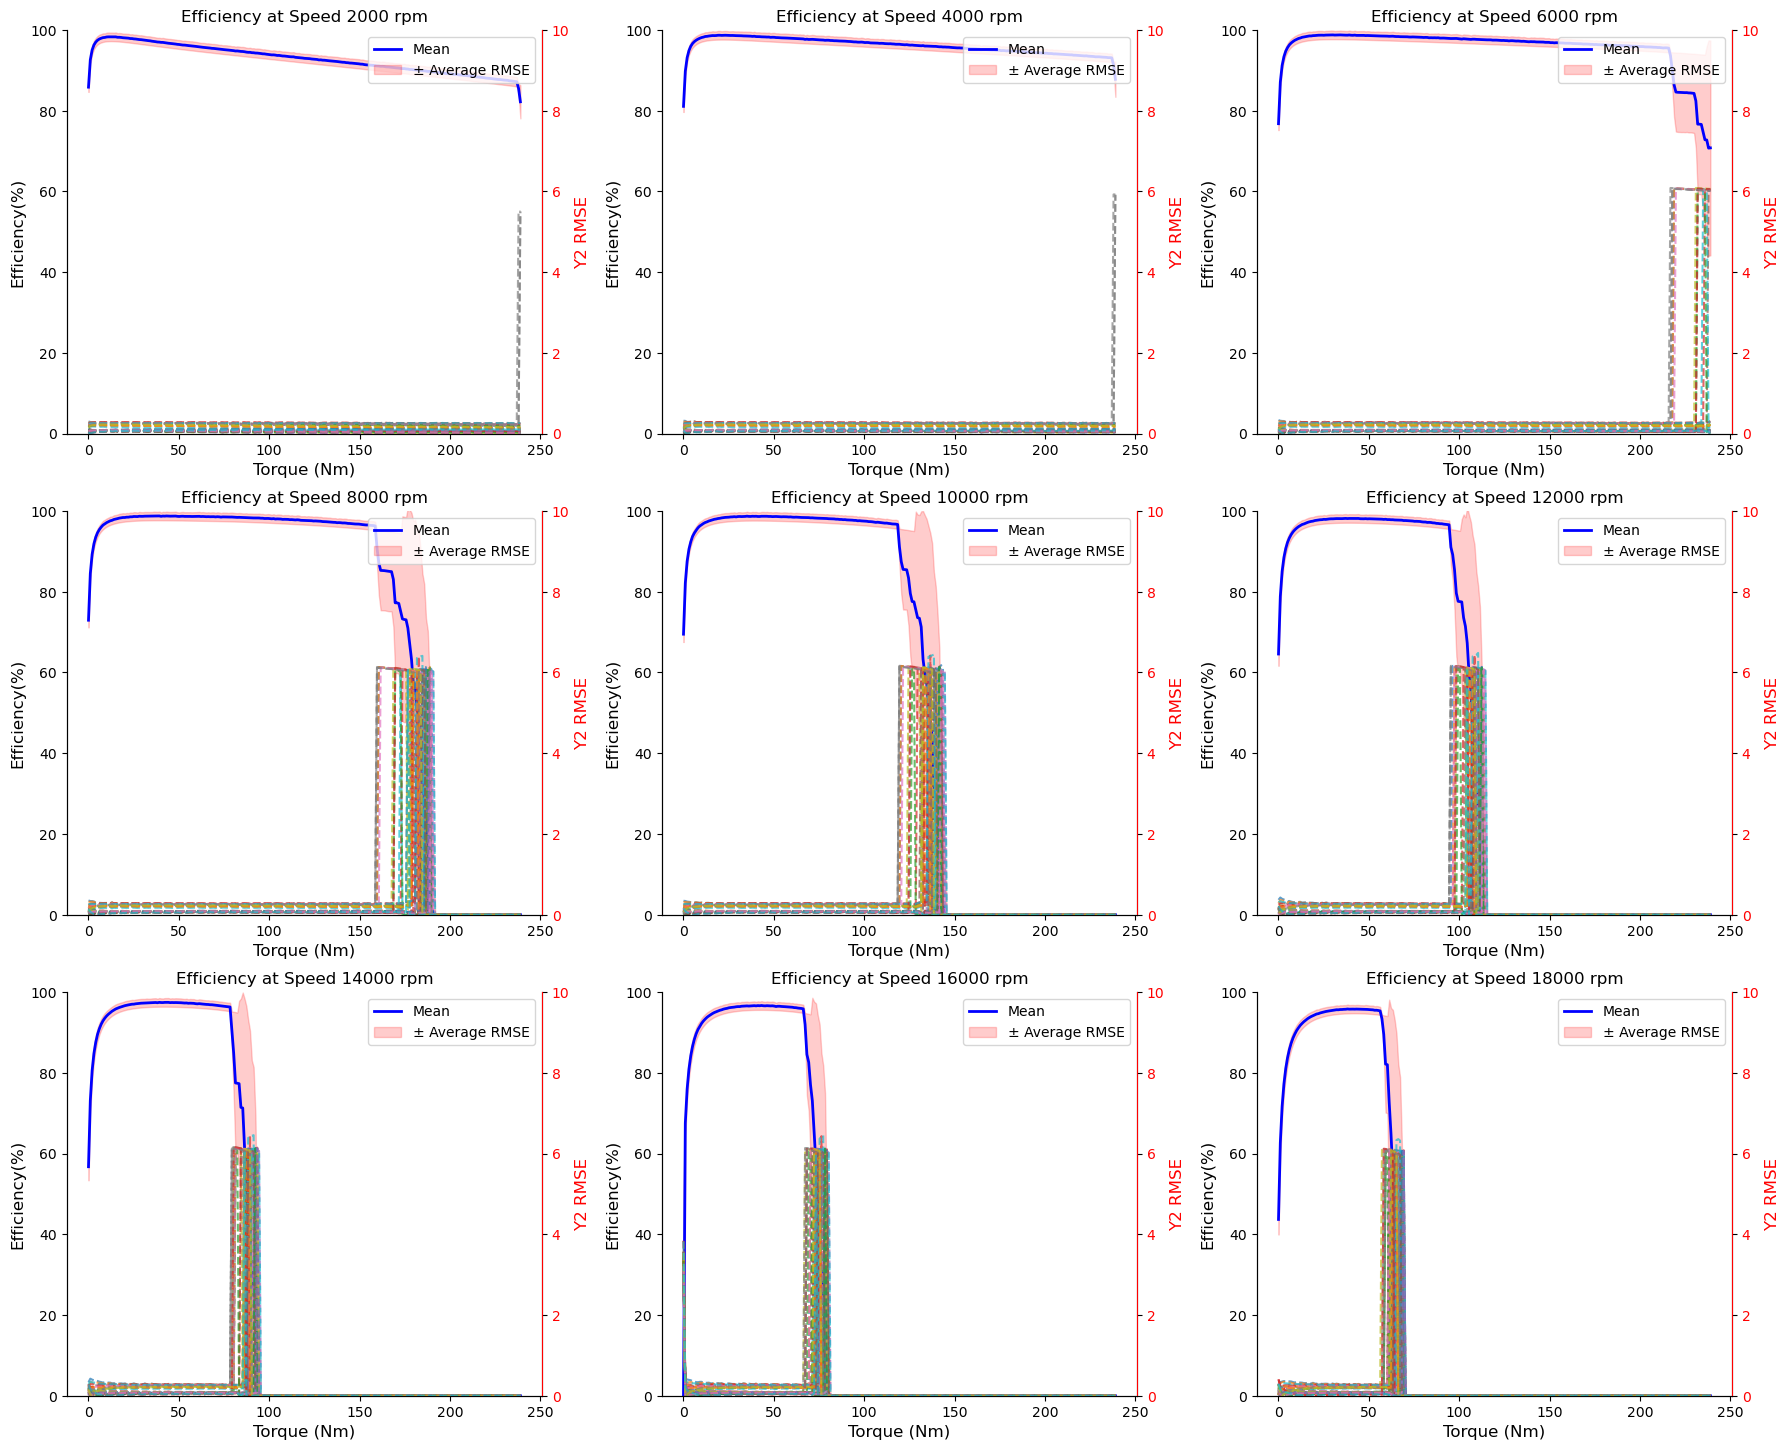
\includegraphics[width=1\textwidth]{./ReportImages/rmse_eta_no_lossreg_MLP.png} 
    \caption{Eval 0 Loss Regularization ETA \ac{RMSE} \ac{KPI}} 
    \label{fig:Eval 0 Loss Regularization ETA RMSE KPI}
\end{figure}

\section{Ablation Studies}\label{sec:Ablation Studies}

As part of ablation studies, we have compared our evaluations of both  \ac{MLP} with different Regularizaions and the Baseline model on both targets respectively.

\begin{minipage}[t]{\textwidth}
    \begin{table}[H]
        \centering
        \begin{tabular}{|l|l|l|}
        \hline {\bf Model} & {\bf Y1 Score} & {\bf Y2 Score}\\
        \hline 
        Baseline & 4.8201 & 15.3708 \\
        MLP\footnote{\centering MLP With Decreasing Y1 Loss Regularization} & 6.0652 & 13.0469 \\
        MLP\footnote{\centering MLP With Smoothening Y1 Loss Regularization} & 5.5052 & 15.0257 \\
        MLP\footnote{\centering MLP without both Y1 and Y2 Loss Regularization} & 4.9887 & 12.6612  \\
        \hline
        \end{tabular}
        \caption{Ablation Studies}
        \label{tab:Ablation Studies}
    \end{table}
\end{minipage}

\vspace{1em} % Adjust the space here, e.g., 1em or 2em

We draw the inferences that our \ac{MLP} model without loss regularization has performed in par with the Baseline on the Mgrenz \ac{KPI} and has outperformed the Baseline on the ETA \ac{KPI}.\\
This could be because the regularizations are restrictive and discourage the model to learn better.\\
The inferences shown are strictly speaking from the Double V Magnet Topology which assumed the bulk of the data we had received.

We have used Python 3.10.14 for our development and the Pytorch library compatible with Cuda.\\
The model was trained on a NVIDIA Tesla V100 \ac{GPU} with 32 GB Memory.\\
Source code is available at the \href{https://github.com/Lilly-25/Masters-Thesis}{GitHub Repository}.

\newpage 

\chapter{Conclusion}

This thesis offers a fresh outlook to the possibility of modelling the performance of an \ac{EM} using \ac{GNN}s.
We have developed a topology invariant \ac{MLP} model to predict 2 \ac{KPI}'s of an \ac{EM} from its parameteric requirements. 
It would be very beneficial to \ac{EM} manufacturers to understand the operating range of the vehicle using the motor and make calculated assumptions of whether to manufacture it.\\
This work enables \ac{EM} designers to generate \ac{KPI}'s at almost both negligible costs and minimal time.
Thus offering an escape from the cons of using \ac{FEM} simulations.\\
It also lays the foundation for future work on being able to generate electric motor design parameters conditioned on the 2 KPIs we predicted.

\section{Future Improvements}\label{sec:Future Improvements}

I would suggest the following improvements to our study : 

\begin{enumerate}
    \item Build a model that uses the Mgrenz \ac{KPI} prediction to predict its corresponding ETA \ac{KPI}. 
    \item Although we have designed the model to be topology invariant for 3 topologies, we only had sufficient data from Double V Topology to draw evaluations from.
    Further evaluations on the other topologies would be beneficial to critically assess our model's performance.
    \item Another interesting study would be to benchmark model performance when one backpropagates the losses for each \ac{KPI} individually rather than weighing them.
    \item Additionally, the motivation of building a topology invariant model was the reason we have considered building a heterogeneous graph to model the data. The machinery is elaborated in Section \ref{sec:EM Heterogeneous GNN Model}.
    Such a model could serve as yet another ablation study to our problem.
\end{enumerate}

\newpage 

\newpage 

\chapter*{Appendix}
\textbf{Node types}

\begin{enumerate}
    \item \textbf{General}
    
    \begin{itemize}
        \item General parameters:
        \[
            r = \{r_{i}\} \quad \forall i \in \{a, r, o\} 
        \]
        
        \textit{where:
        \begin{itemize}
            \item $r_{a}$: Outer Radius of the Stator
            \item $r_{r}$: Outer Radius of the Rotor
            \item $r_{o}$: Center of the \ac{EM}
        \end{itemize}}
    \end{itemize}
    
    \item \textbf{Stator}
    
    \begin{itemize}
        \item Slot windings:
        \[
            sw = \{s_{i}w_{j}\} \quad \forall i \in \{1, \dots, QSim\}, \quad \forall j \in \{1, \dots, N\} 
        \]
        
        \item Slots:
        \[
            s = \{s_{i}\} \quad \forall i \in \{1, \dots, QSim\}
        \]

        \textit{where
        \begin{itemize}
            \item Qsim : Count of slots in the Stator
            \item N : Count of copper windings per slot
        \end{itemize}}
    \end{itemize}
    
    \item \textbf{Rotor}
    
    \begin{itemize}
        \item Magnet Flux Barriers:
        \[
            v = \{v_{ij}\} \quad \forall i \in \{1, \dots, T\}, \quad \forall j \in \{1, \dots, V\}
        \]
        
        \item Magnets:
        \[
            vm = \{v_{i}m_{j}\} \quad \forall i \in \{1, \dots, T\}, \quad \forall j \in \{1, \dots, V\}
        \]
        \textit{where
        \begin{itemize}
            \item T : Topology type of the \ac{EM}
            \item V : Type of Magnet
        \end{itemize}
        As Valeo only manufactures Double V magnets we consider it to be 2}
    \end{itemize}    
    
\end{enumerate}

\textbf{Edge types}

\begin{enumerate}
    \item \textbf{Angle} \\
    \textbf{Relevant Paths}
    \[
    vm--vm = \{ v_{i_{1}}m_{j_{1}} - v_{i_{2}}m_{j_{2}} \}
    \forall i_1, i_2 \in \{1, \dots, T\}, \quad \forall j_1, j_2 \in \{1, \dots, V\} \mid
    i_1 = i_2, \quad j_1 \neq j_2
    \]

    \textbf{angle}=vm-vm

    \item \textbf{Distance} \\
    \textbf{Relevant Paths}
    % \[
    %     v-v = \{ (v_{i_1 j_1} - v_{i_2 j_2}), \forall i_1, i_2, j_1, j_2 \in \{1, \dots, T\} \mid i_1i_2 \neq j_1j_2 \ \land (i_1 == i_2 \lor j_1 == j_2) \}
    % \]
    \[
        vi--vi = \{v_{i j_1} - v_{i j_2}\}, \forall i \in \{1, \dots, T\}, \forall j_1, j_2 \in \{1, \dots, V\} \mid  j_1 \neq j_2
    \]
    \[
        vi--vj = \{v_{i_1 j} - v_{i_2 j}\}, \forall i_1, i_2 \in \{1, \dots, T\}, \forall j \in \{1, \dots, V\} \mid  i_1 \neq i_2
    \]
    \[
        v--vm = \{v_{i j} - v_{i}m_{j}\} \forall i  \in \{1, \dots, T\}, \quad \forall j \in \{1, \dots, V\}
    \]
    \[
        v--rr = \{v_{i j} - r_{r}\}, \forall i, j  \in \{1, \dots, T\}
    \]
    \[
        o--r = \{ (o - r_{r}), (o - r_{a})\}
    \]
    \[
        rr--s = \{r_{r} - s_{i}\}, \forall i  \in \{1, \dots, QSim\}
    \]
    \[
        s--sw = \{s_{i} - s_{i}w_{j}\}, \forall i  \in \{1, \dots, QSim\}, \forall j  \in \{1, \dots, N\}
    \]
    \[
        s--ra = \{s_{i} - r_{a}\}, \forall i  \in \{1, \dots, QSim\}
    \]
    \[
        sw--sw = \{s_{i}w_{j_1} - s_{i}w_{j_2}\}, \forall i  \in \{1, \dots, QSim\}, \forall j  \in \{1, \dots, N\} \mid (j_1 == j_2-1)
    \]

    \textbf{distance} = vi--vi + vi--vj + v--vm + v--rr + o--r + rr--s + s--sw + s--ra + sw--sw

\end{enumerate}

\textbf{Node Features}

\begin{enumerate}

    \item \textbf{v} = \{lmsov, lth1v, lth2v, r1v, r11v, r2v, r3v, r4v, rmt1v, rmt4v, rlt1v, rlt4v, hav\}

    \item \textbf{vm} = \{mbv, mhv, rmagv\}

    \item \textbf{r} = \{r\}

    \item \textbf{s} = \{b\_nng, b\_nzk, b\_s, h\_n, h\_s, r\_sn, r\_zk, r\_ng, h\_zk\}

    \item \textbf{sw} = \{bhp, hhp, rhp\}
\end{enumerate}

\textbf{Path Features}

\begin{enumerate}

    \item \textbf{vm--vm} = \{deg\_phi\}

    \item \textbf{vi--vi} = \{dsm, dsmu\}

    \item \textbf{vi--vj} = \{amtrvj-amtrvi\}

    \item \textbf{v--vm} = \{lmav, lmiv, lmov, lmuv\}

    \item \textbf{v--r} = \{amtrv, dsrv\}
    
    \item \textbf{o--r} = \{r\}

    \item \textbf{rr--s} = \{airgap\}

    \item \textbf{s--sw} = \{dhphp\}
    
    \item \textbf{sw--sw} = \{dhpng\}
    
    \item \textbf{s--ra} = \{r\_a-(r\_i + h\_n + h\_zk)\}
    
\end{enumerate}


\listoffigures

\newpage 

\newpage 

\listoftables

\newpage 

\newpage 

\begin{thebibliography}{00}

    \bibitem[01]{EHR HGNN-2024}
    \newblock Tsai Hor Chana, Guosheng Yina, Kyongtae Baeb, Lequan Yu 
    \newblock {\em Multi-task Heterogeneous Graph Learning on Electronic Health Records}.
    \newblock cs.LG, 14 Aug 2024.
    
    \bibitem[02]{SE HGNN-2023}
    \newblock Xiaocheng Yang, Mingyu Yan, Shirui Pan, Xiaochun Ye, Dongrui Fan
    \newblock {\em Simple and Efficient Heterogeneous Graph Neural Network}.
    \newblock cs.LG, 1 Sep 2023.

    \bibitem[03]{EV HGNN-2023}
    \newblock Xinru Huang
    \newblock {\em A Heterogeneous Graph Neural Network Model for Electric Vehicle Purchase Propensity Prediction}.
    \newblock ICDSCA, Oct 2023.
    
    \bibitem[04]{REF HGNN-2021}
    \newblock Qingsong Lv, Ming Ding, Qiang Liu, Yuxiang Chen, Wenzheng Feng, Siming He, Chang Zhou, Jianguo Jiang, Yuxiao Dong, Jie Tang
    \newblock {\em Are we really making much progress? Revisiting, benchmarking, and refining heterogeneous graph neural networks}.
    \newblock cs.LG, 30 Dec 2021.

    \bibitem[05]{ML HGNN-2023}
    \newblock Fredrik Johannessen; Martin Jullum
    \newblock {\em Finding Money Launderers Using Heterogeneous Graph Neural Networks}.
    \newblock ICDSCA, 25 July 2023.
    
    \bibitem[06]{PO GNN-2018}
    \newblock Damian Owerko, Fernando Gama, Alejandro Ribeiro
    \newblock {\em Predicting Power Outages Using Graph Neural Networks}.
    \newblock cs.LG, Nov 2018.

    \bibitem[07]{SM EMT-2020}
    \newblock Mikko Tahkola, Janne Keränen, Denis Sedov, Mehrnaz Farzam Far, Juha Kortelainen
    \newblock {\em Surrogate Modeling of Electrical Machine Torque Using Artificial Neural Networks}.
    \newblock ICDSCA, Dec 17 2020.
    
    \bibitem[08]{EM 2DFMP-2022}
    \newblock AKM Khaled Ahsan Talukder, Bingnan Wang and Yusuke Sakamoto
    \newblock {\em Electric Machine Two-dimensional Flux Map Prediction with Ensemble Learning}.
    \newblock ICEMS, 2022.

    \bibitem[09]{T-CNN-2024}
    \newblock Kazuhisa Iwata, Hidenori Sasaki, Hajime Igarashi, Daisuke Nakagawa, and Tomoya Ueda
    \newblock {\em Generalization Performance in Predicting Torque Characteristics Using Convolutional Neural Network and Stator Magnetic Flux.}
    \newblock ICDSCA, 3 Mar 2024.
    
    \bibitem[10]{EM MP-2021}
    \newblock Simone Ferrari, Paolo Ragazzo, Gaetano Dilevrano, Gianmario Pellegrino
    \newblock {\em Flux-Map Based FEA Evaluation of Synchronous Machine Efficiency Maps}.
    \newblock WEMDCD, 2021.

    \bibitem[11]{EM 2DFMP-2021}
    \newblock Vivek Parekh, Dominik Flore, Sebastian Schöps
    \newblock {\em Deep Learning-Based Prediction of Key Performance Indicators for Electrical Machines}.
    \newblock Jan 22, 2021.

    \bibitem[12]{EMAP-2020}
    \newblock Carlos Candelo-Zuluaga, Antonio Garcia Espinosa, Jordi-Roger Riba, Pere Tubert Blanch
    \newblock {\em Computationally Efficient Analysis of Spatial and Temporal Harmonics Content of the Magnetic Flux Distribution in a PMSM for Efficiency Maps Computation.}
    \newblock 2020.
    
    \bibitem[13]{EM SM-2023}
    \newblock Yihao Xu, Bingnan Wang, Yusuke Sakamoto, Tatsuya Yamamoto, and Yuki Nishimura
    \newblock {\em Comparison of Learning-based Surrogate Models for Electric Motors}.
    \newblock COMPUMAG, 2023.

    \bibitem[14]{IM HML-2021}
    \newblock Marius Stender, Oliver Wallscheid, Joachim Böcker
    \newblock {\em Accurate Torque Estimation for Induction Motors by Utilizing a Hybrid Machine Learning Approach}.
    \newblock PEMC, 2021.

    \bibitem[15]{EM FEM-2020}
    \newblock Katsuyuki Narita, Hiroyuki Sano, Nicolas Schneider, Kazuki Semba, Koji Tani, Takashi Yamada, Ryosuke Akaki
    \newblock {\em An Accuracy Study of Finite Element Analysis- based Efficiency Map for Traction Interior Permanent Magnet Machines}:
    \newblock 2020.
    
    \bibitem[16]{EM TL-2020}
    \newblock Jo Asanuma, Shuhei Doi, Hajime Igarashi
    \newblock {\em Transfer Learning Through Deep Learning: Application to Topology Optimization of Electric Motor}.
    \newblock 3 Mar 2020.

    \bibitem[17]{ADAM-2017}
    \newblock Diederik P. Kingma, Jimmy Ba
    \newblock {\em Adam: A Method for Stochastic Optimization}.
    \newblock 30 Jan 2017.

    \end{thebibliography}
\newpage 

\newpage 

\chapter*{Declaration on oath}
\addcontentsline{toc}{chapter}{Declaration on oath}

\vspace{1cm}

\noindent I hereby certify that I have written my master thesis independently and have not yet submitted it for examination purposes elsewhere. All sources and aids used are listed, literal and meaningful quotations have been marked as such.

\vspace{3cm}
\hfill\rule{15cm}{0.4pt} % Horizontal line for the signature aligned to the right

\begin{center}
    Lilly Abraham K64889, 11.12.2024 % Placeholder for the signature and date
\end{center}

\newpage 

\chapter*{Consent to Plagiarism Check}
\addcontentsline{toc}{chapter}{Consent to Plagiarism Check}
\vspace{1cm}

\noindent I hereby agree that my submitted work may be sent to PlagScan (www.plagscan.com) in digital form for the purpose of checking for plagiarism and that it may be temporarily (max. 5 years) stored in the database maintained by PlagScan as well as personal data which are part of this work may be stored there.

\vspace{0.5cm}

\noindent Consent is voluntary. Without this consent, the plagiarism check cannot be prevented by removing all personal data and protecting the copyright requirements. Consent to the storage and use of personal data may be revoked at any time by notifying the faculty.

\vspace{3cm}
\hfill\rule{15cm}{0.4pt} % Horizontal line for the signature aligned to the right

\begin{center}
    Lilly Abraham K64889, 11.12.2024 % Placeholder for the signature and date
\end{center}

\end{document}
